\documentclass[12pt,twoside,openright,a5paper]{book}
\usepackage[margin=0.75in]{geometry}
\usepackage{layout}
\usepackage{pgffor}
\usepackage{tocloft}
\usepackage[table, dvipsnames]{xcolor}
\usepackage{fontspec}
\usepackage{fancybox}
\usepackage[skins]{tcolorbox}
\usepackage{fancyhdr}
\usepackage{setspace}
\usepackage[utf8]{inputenc}
\usepackage{emptypage}
\usepackage[vskip=0pt,rightmargin=0cm]{quoting}
\usepackage{sectsty}
\usepackage{polyglossia}
\usepackage{changepage}%
\usepackage{imakeidx}
\usepackage{setspace}
\usepackage{longtable,array}
\usepackage{tikz} % Package for drawing
\usepackage{tikzpagenodes}
\usepackage[toc,acronym]{glossaries}
\usepackage{fontawesome5}
\usepackage{marvosym}
\usepackage[totoc, font=footnotesize]{idxlayout}
\usepackage{eso-pic} % background image in titlepage
\usepackage{anyfontsize} % any font size
% Remove this package for the final copy
\newfontfamily\engfont[Script=Kannada]{Arial Unicode MS}
\usepackage[hpos=24mm,fontsize=32pt, hanchor=l,anchor=lc,angle=90,color={[gray]{0.5}}, text={\engfont{DRAFT \ COPY}}]{draftwatermark}




\newfontfamily\engfont[Script=Kannada]{Arial Unicode MS}
\usepackage[hpos=24mm,fontsize=32pt, hanchor=l,anchor=lc,angle=90,color={[gray]{0.5}}, text={\engfont{DRAFT \ COPY}}]{draftwatermark}

\newskip\linepagesep \linepagesep 5pt\relax
\renewcommand\footrulewidth{0.5pt}
\def\vfootline{%
    \begingroup
        \color{blue}\rule[-990pt]{20pt}{1000pt}
    \endgroup}



\setmainfont[Script=Kannada, Renderer=HarfBuzz]{Noto Serif Kannada}
\setmainlanguage[numerals=kannada]{kannada}
\setotherlanguages{english}
\newfontfamily\kannadafont[Script=Kannada]{Noto Serif Kannada}
\newfontfamily\kannadafontsf[Script=Kannada]{Noto Serif Kannada}
\newfontfamily\kanBold[Script=Kannada]{Noto Serif Kannada Bold}
\newfontfamily\kanfont[Script=Kannada]{Noto Serif Kannada}
\newfontfamily\mananamfont[Script=Kannada]{NudiUni08k}
\newfontfamily\mananatext[Script=Kannada]{AdishilaVedic}
\fancyhf{}
  \fancyfoot[RO]{\vfootline\hskip\linepagesep\thepage}
  \fancyfoot[LE]{\thepage\hskip\linepagesep\vfootline}
  \fancyhead[RO]{\small\kanfont ದಿನಾಂಕ ..../..../.....}
  \fancyhead[LO]{\small\kanfont ಗೀತಾ ಮನನಂ (ಮಾದರಿ ಪ್ರತಿ)}
  \fancyhead[LE]{\small\kanfont ಗೀತಾ ಮನನಂ (ಮಾದರಿ ಪ್ರತಿ)}
  \fancyhead[RE]{\small\kanfont ದಿನಾಂಕ ..../..../.....}
  \renewcommand\headrulewidth{1pt}
  \fancypagestyle{plain}{%
    \fancyhf{}
    \fancyfoot[RO]{\vfootline\hskip\linepagesep\thepage}
    \fancyfoot[LE]{\thepage\hskip\linepagesep\vfootline}
    \renewcommand\headrulewidth{0pt}
  }
\quotingsetup{font={itshape,footnotesize}}
\title{\Huge \kanfont \textbf{ಗೀತಾ ಮನನಂ}\\
{\normalsize Gita Mananam\\}
{\small(ದೈನಂದಿನ ಸ್ಪೂರ್ತಿ ಹಾಗೂ ಆತ್ಮಾವಲೋಕನಕ್ಕಾಗಿ)}}
\author{\large \kanfont ಸ್ವಾಮಿ ನಿರ್ಗುಣಾನಂದಗಿರಿ\\
{\normalsize Swamy Nirgunanandagiri}\\
\vspace{15mm}
{\normalsize Bhageeratha Publications}\\
{Rishikesh, India}
}


\addto\captionskannada{\renewcommand{\contentsname}{\color{blue}{ವಿಷಯ ಸೂಚಿ}}} 

% Reduce space between TOC
\setlength\cftparskip{-2pt}
\setlength\cftbeforechapskip{2pt}
\setcounter{secnumdepth}{-1}
\chapterfont{\color{blue}}  % sets colour of chapters
\setlength\parindent{0pt} % no-indent for entire file
\date{} % clear date
\makeindex
\indexsetup{othercode=\small}
%%Term definitions
\mananatext{
\begin{description}
   \item[ಧರ್ಮ] ಧರ್ಮವೆಂಬುವುದು ಸಾಮಾನ್ಯತಃ, ಒಬ್ಬ ವ್ಯಕ್ತಿಯ ಜೀವನದಲ್ಲಿ, ಸಮಾಜದಲ್ಲಿ ಹಾಗೂ ಪ್ರಕೃತಿಯ ನಿಯಮಕ್ಕೆ ಹೊಂದಿಕೊಂಡು ಹೋಗುವಂತಹ, ಅವನ ನೈತಿಕ ಬಾಧ್ಯತೆ ಕರ್ತವ್ಯಗಳ ಮಹತ್ವವನ್ನು ಸೂಚಿಸುತ್ತದೆ. ಗೀತೆ ಮತ್ತು ವೇದಗಳ ದೃಷ್ಟಿಕೋನದಿಂದ ನೋಡಿದರೆ, ಕೇವಲ ಲೌಕಿಕ ಲಾಭಗಳಿಗೆ ಮಾತ್ರವಲ್ಲದೇ, ಆಧ್ಯಾತ್ಮಿಕ ಜೀವನ ಮತ್ತು ಮೋಕ್ಷದ ಅನ್ವೇಷಣೆಗಾಗಿ ಧರ್ಮದ ಪರಿಪಾಲನೆ ಮಾಡುವುದೇ ಆಗಿದೆ. ಅಹಂ ಮತ್ತು ಅದರ ಇಷ್ಟಾನಿಷ್ಟಗಳನ್ನು ಮೆಟ್ಟಿ, ಈ ಸೃಷ್ಟಿಯ ದೈವೀಕ ಯೋಜನೆಗೆ ಅನುಗುಣವಾಗಿ ಜೀವಿಸುವುದೇ ಧರ್ಮದ ಕರೆಯಾಗಿದೆ.
   \item[ಭಗವಂತ] ಭಗವಾನ್ ಎಂದರೆ, ಆರು ದೈವೀಕ ಗುಣಗಳಾದ  ಪ್ರಭುತ್ವ, ಅಧಿಕಾರತ್ವ, ಖ್ಯಾತಿ, ಶಕ್ತಿ, ಜ್ಞಾನ ಮತ್ತು ತಟಸ್ಥತೆ ಹೊಂದಿರುವ ಒಂದು  ಪದವಿ. ಗೀತೆಯಲ್ಲಿ ಭಗವಾನ್ ಎಂದರೆ,  ‘ಪರಮಗುರು’;  ಸಾಕಾರ ರೂಪದಲ್ಲಿರುವ ಆ ಪರಮಾತ್ಮನೇ; ಗ್ರಹಣಾಕಾಂಕ್ಷಿಯಾದ ಸಾಧಕನಿಗೆ ಕರುಣೆಯಿಂದ ಮುಕ್ತಿಮಾರ್ಗಕ್ಕೆ ಬೇಕಾದ ವಿವೇಕವನ್ನು ದಯಪಾಲಿಸುವವನು ; ಶ್ರದ್ಧಾಳು ಭಕ್ತರಿಗೆ ಭಗವಂತನೆಂದರೆ ಪರಮ ಆಶ್ರಯದಾತನು ಹಾಗೂ, ಆತ್ಮಸಾಕ್ಷಾತ್ಕಾರಕ್ಕಾಗಿ ಮಾರ್ಗವನ್ನು ತೋರಿಸುವ ದೀವಿಗೆ.
   \item[ಸ್ಥಿತಪ್ರಜ್ಞ] ಯಾವ ವ್ಯಕ್ತಿಗೆ ಸ್ಥಿರವಾದ ವಿವೇಕ ಮತ್ತು ಬುದ್ಧಿಶಕ್ತಿ ಇರುವುದೋ, ಯಾರು ಸದಾ ಸಮಚಿತ್ತತೆಯಿಂದ ಇರುವನೋ, ಯಾರ ಇಂದ್ರಿಯಗಳು ಅವನ ಹಿಡಿತದಲ್ಲಿರುವುವೋ, ಯಾರು ಆಸೆ ಮತ್ತು ಭಯದಿಂದ ಮುಕ್ತನೋ ಹಾಗೂ, ಜೀವನದಲ್ಲಿ ಸಂತೋಷ ಬಂದಾಗ ತೀರಾ ಹಿಗ್ಗದೇ, ದುಃಖ ಬಂದಾಗ ಹತಾಶನಾಗದೇ ಇರುವನೋ,ಅಂಥವನು ‘ಸ್ಥಿತಪ್ರಜ್ಞ’ ; ಅಲ್ಲದೇ, ಯಾವನು ತನ್ನ ಆತ್ಮದಲ್ಲಿಯೇ ಸಂತೃಪ್ತನೋ, ಹಾಗೂ ಸಾಮಾನ್ಯತಃ, ಆತ್ಮಜ್ಞಾನವಿಲ್ಲದ ಒಬ್ಬನಿಗೆ ಕಾಡುವ ಅಪೂರ್ಣತೆಯ ಭಾವನೆ ಯಾವನಿಗೆ ಇಲ್ಲವೋ, ಅವನೇ ‘ಸ್ಥಿತಪ್ರಜ್ಞ’ ಎಂದೆನಿಸಿಕೊಳ್ಳುತ್ತಾನೆ.
\end{description}
}
%\makeglossaries


\newcommand\Linepage[1][0.40in]{% Change to suit
  \vbox to \dimexpr\textheight-\pagetotal-#1\relax {% Let TeX do the work...
    \leaders\hbox to \linewidth{\rule{0pt}{#1}\hrulefill}\vfil
  }%
}

\newtcolorbox{inspiration}[2][]{%
  floatplacement=b,float, 
  enhanced,colback=white,colframe=purple,coltitle=black,
  sharp corners,boxrule=1pt, width=\textwidth,
  fonttitle=\sffamily\scshape\color{teal},
  rightrule=3mm,
  fontupper=\itshape,
  fontlower=\tiny,
  attach boxed title to top left={yshift=-0.5\baselineskip-0.4pt,xshift=2mm},
  boxed title style={tile,size=minimal,left=0.5mm,right=0.5mm,
    colback=white,before upper=\strut},
  title=#2,#1
}
\newtcolorbox{mananam}[2][fontlower=\small]{%
  enhanced,colback=white,colframe=teal,coltitle=black,
  sharp corners,boxrule=1pt, width=\textwidth,
  fonttitle=\sffamily\scshape\color{purple},
  leftrule=3mm,
  fontupper=\itshape,
  fontlower=\tiny,
  attach boxed title to top left={yshift=-0.5\baselineskip-0.4pt,xshift=4mm},
  boxed title style={tile,size=minimal,left=0.5mm,right=0.5mm,
    colback=white,before upper=\strut},
  title=#2,#1
}



% commands
\definecolor{aurometalsaurus}{rgb}{0.43, 0.5, 0.5}
\newcommand{\slcol}[1]{{\color{MidnightBlue}{#1}}}
\newcommand{\cquote}[1]{\begin{quoting}{\color{black}{#1}}\end{quoting}}
%% Custom macro to convert Arabic numerals to Kannada numerals
\makeatletter
\newcommand{\converttoKannada}[1]{%
  \ifcase#1 ೦\or ೧\or ೨\or ೩\or ೪\or ೫\or ೬\or ೭\or ೮\or ೯\else\expandafter\converttoKannadaLoop\fi
}
\newcommand{\converttoKannadaLoop}[1]{%
  \expandafter\converttoKannada\expandafter{\the\numexpr#1/10}\converttoKannada{\the\numexpr#1\mod10}%
}
\makeatother

% Redefine page numbering globally to use Kannada numerals
\renewcommand{\thepage}{\converttoKannada{\arabic{page}}}

% Redefine index page numbers (the page numbers shown in the index itself)
\renewcommand{\index}{\@ifnextchar[{\@indexwithpage}{\@indexwithoutpage}}

\def\@indexwithpage[#1]#2{\indexentry{#2}{\converttoKannada{#1}}}
\def\@indexwithoutpage#1{\indexentry{#1}{\converttoKannada{\thepage}}}
\renewcommand{\cftchapfont}{\normalfont}
\renewcommand{\cftchappagefont}{\normalfont}
%column decoration
\setlength{\columnseprule}{1pt}
\def\columnseprulecolor{\color{blue}}

\begin{document}

\pagenumbering{roman}
\begin{titlepage}
	%\pagecolor{pastelblue}
	\AddToShipoutPictureBG*{%
    \AtPageLowerLeft{%
        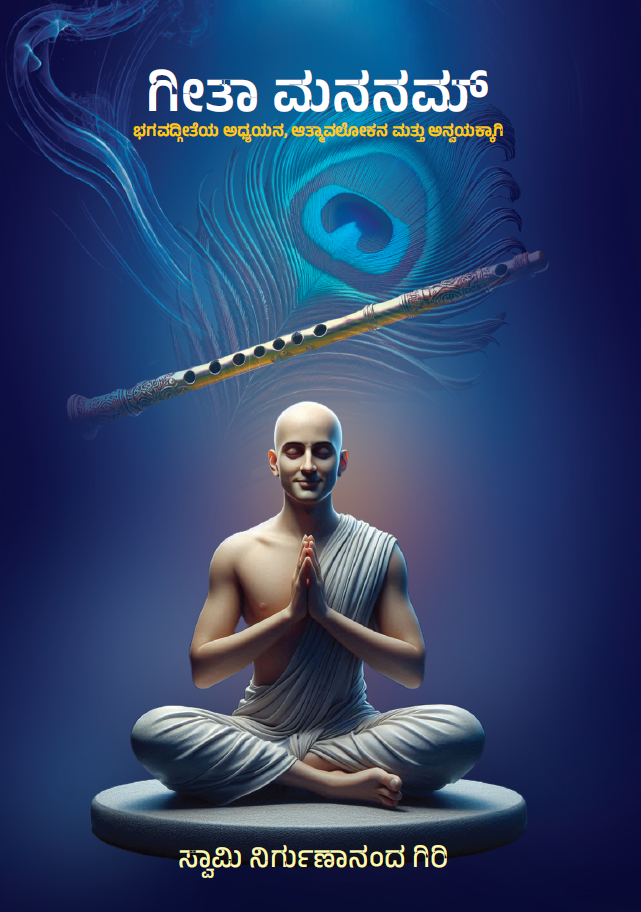
\includegraphics[width=\paperwidth,height=\paperheight]{./images/frontcover.png}%
    }%
}
    \begin{center}
        \vspace*{0.5cm}
            
        {\Huge
        %\textbf{\color{white}\fontsize{50}{60}\selectfont ಗೀತಾ ಮನನಂ}
		}
        %\textbf{\\ \small \color{white}ದೈನಂದಿನ ಸ್ಪೂರ್ತಿ ಹಾಗೂ ಆತ್ಮಾವಲೋಕನಕ್ಕಾಗಿ}    
        \vspace{1.0cm}
            
        
		
            
        \vfill
            
        
            
        \vspace{0.1cm}
        {\color{white}    
		%\textbf{{\Large \mananamfont ಸ್ವಾಮಿ ನಿರ್ಗುಣಾನಂದ ಗಿರಿ}}\\
		%{\normalsize Swami Nirgunananda Giri\\Rishikesh, India}
		}
    \end{center}
\end{titlepage}
\nopagecolor% Use this to restore the color pages to white
\begin{titlepage}
	%\pagecolor{pastelblue}
	%\AddToShipoutPictureBG*{%
    %\AtPageLowerLeft{%
    %    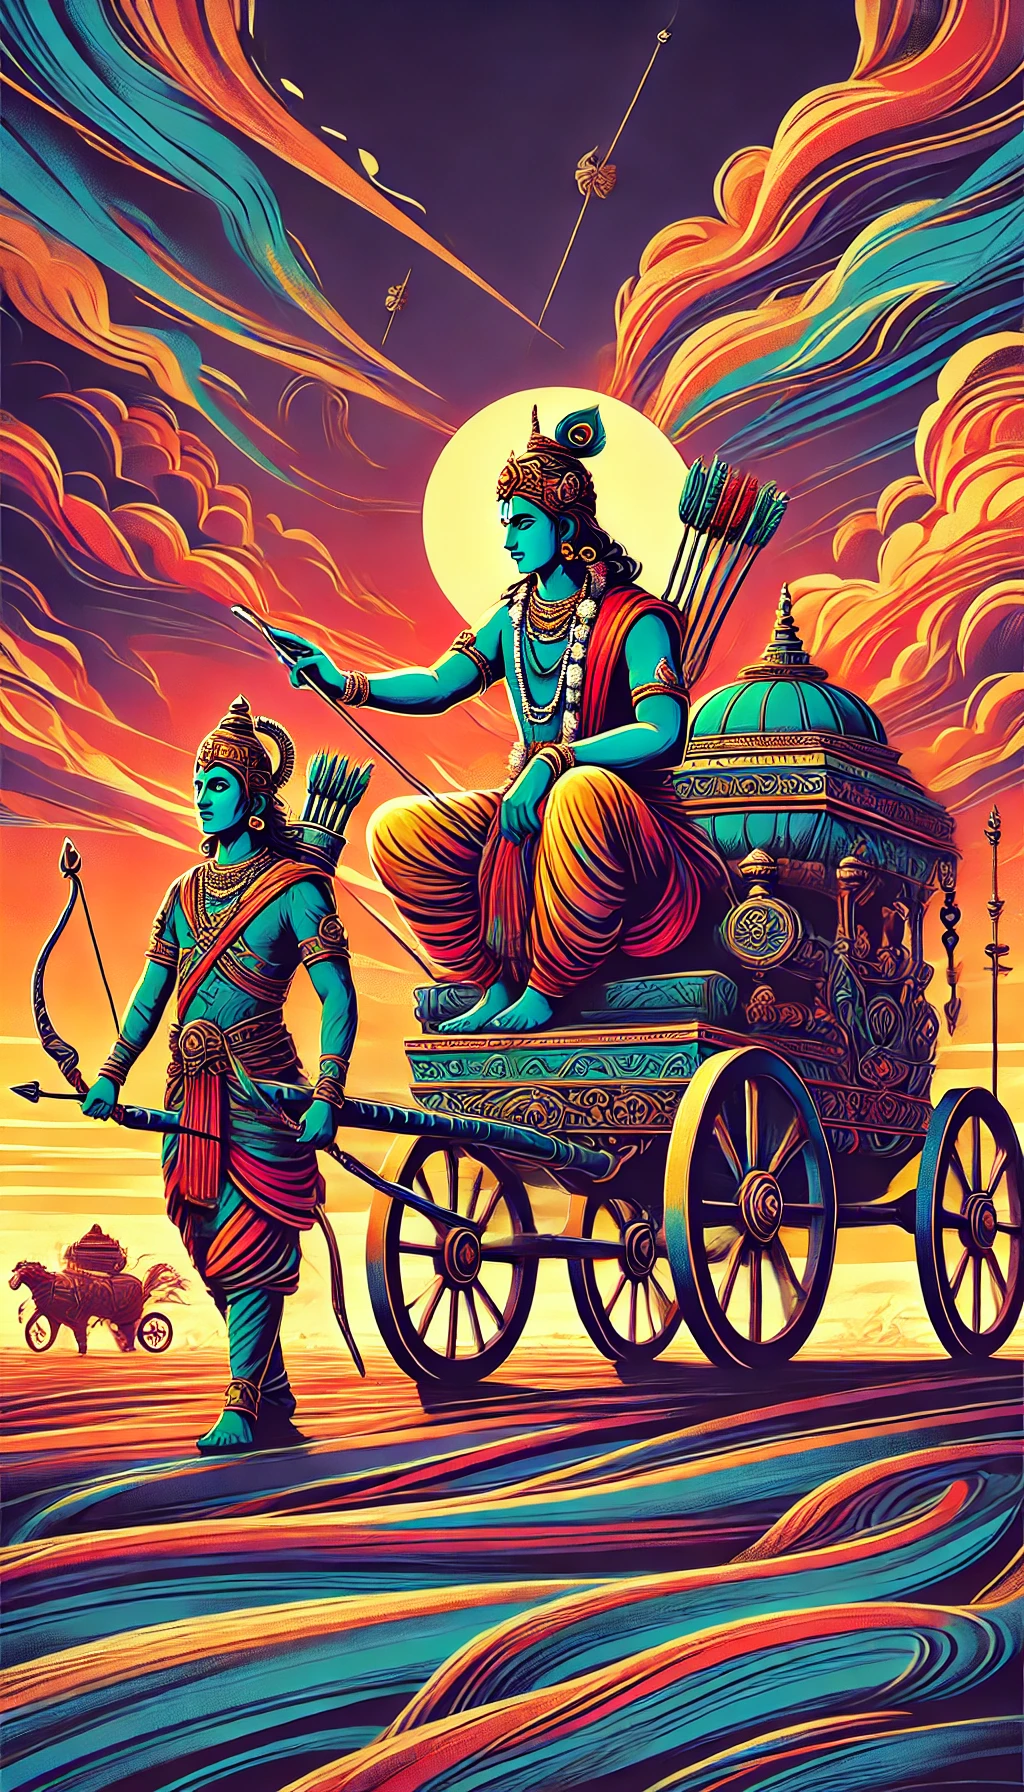
\includegraphics[width=\paperwidth,height=\paperheight]{./images/krishna4.jpg}%
    %}%
%}
    \begin{center}
        \vspace*{0.5cm}
            
        {\Huge
        \textbf{\color{blue}\fontsize{50}{60}\selectfont ಗೀತಾ ಮನನಂ}}
        \textbf{\\ \small \color{black}ದೈನಂದಿನ ಸ್ಪೂರ್ತಿ ಹಾಗೂ ಆತ್ಮಾವಲೋಕನಕ್ಕಾಗಿ}\\    
        \vspace{1.0cm}
		    \textbf{{\large \color{black} ಅಧ್ಯಾಯ ೫ ಕರ್ಮ ಸನ್ಯಾಸ ಯೋಗ}}\\		
        \vspace{6.0cm}
        \textbf{{\Large \color{blue}\mananamfont ಸ್ವಾಮಿ ನಿರ್ಗುಣಾನಂದ ಗಿರಿ}}\\    
        
		
            
        \vfill
            
        
            
        \vspace{0.1cm}
        {\color{black}    
		
		{{\large \color{blue}ಹೃಷೀಕೇಶ, ಉತ್ತರಾ ಖಂಡ}\\\normalsize ಭಾರತ}
        }
    \end{center}
\end{titlepage}
\nopagecolor% Use this to restore the color pages to white
%\maketitle

\thispagestyle{empty}
Copyright \textcopyright\ Swamy Nirgunanandagiri\\
\\
All rights reserved\\
\\
Edition - First, 2024\\
\vfill
Without written permission of the author it is forbidden to reproduce or adapt in any form or by any means any part of this  publication.\\
\\
Rishikesh, India\\
\newpage
\thispagestyle{empty}
\frontmatter

\doublespacing
\tableofcontents
\singlespacing
%\clearpage
%\newgeometry{margin=0pt} % Apply margin only for this page
%\thispagestyle{empty}
%\begin{center}
%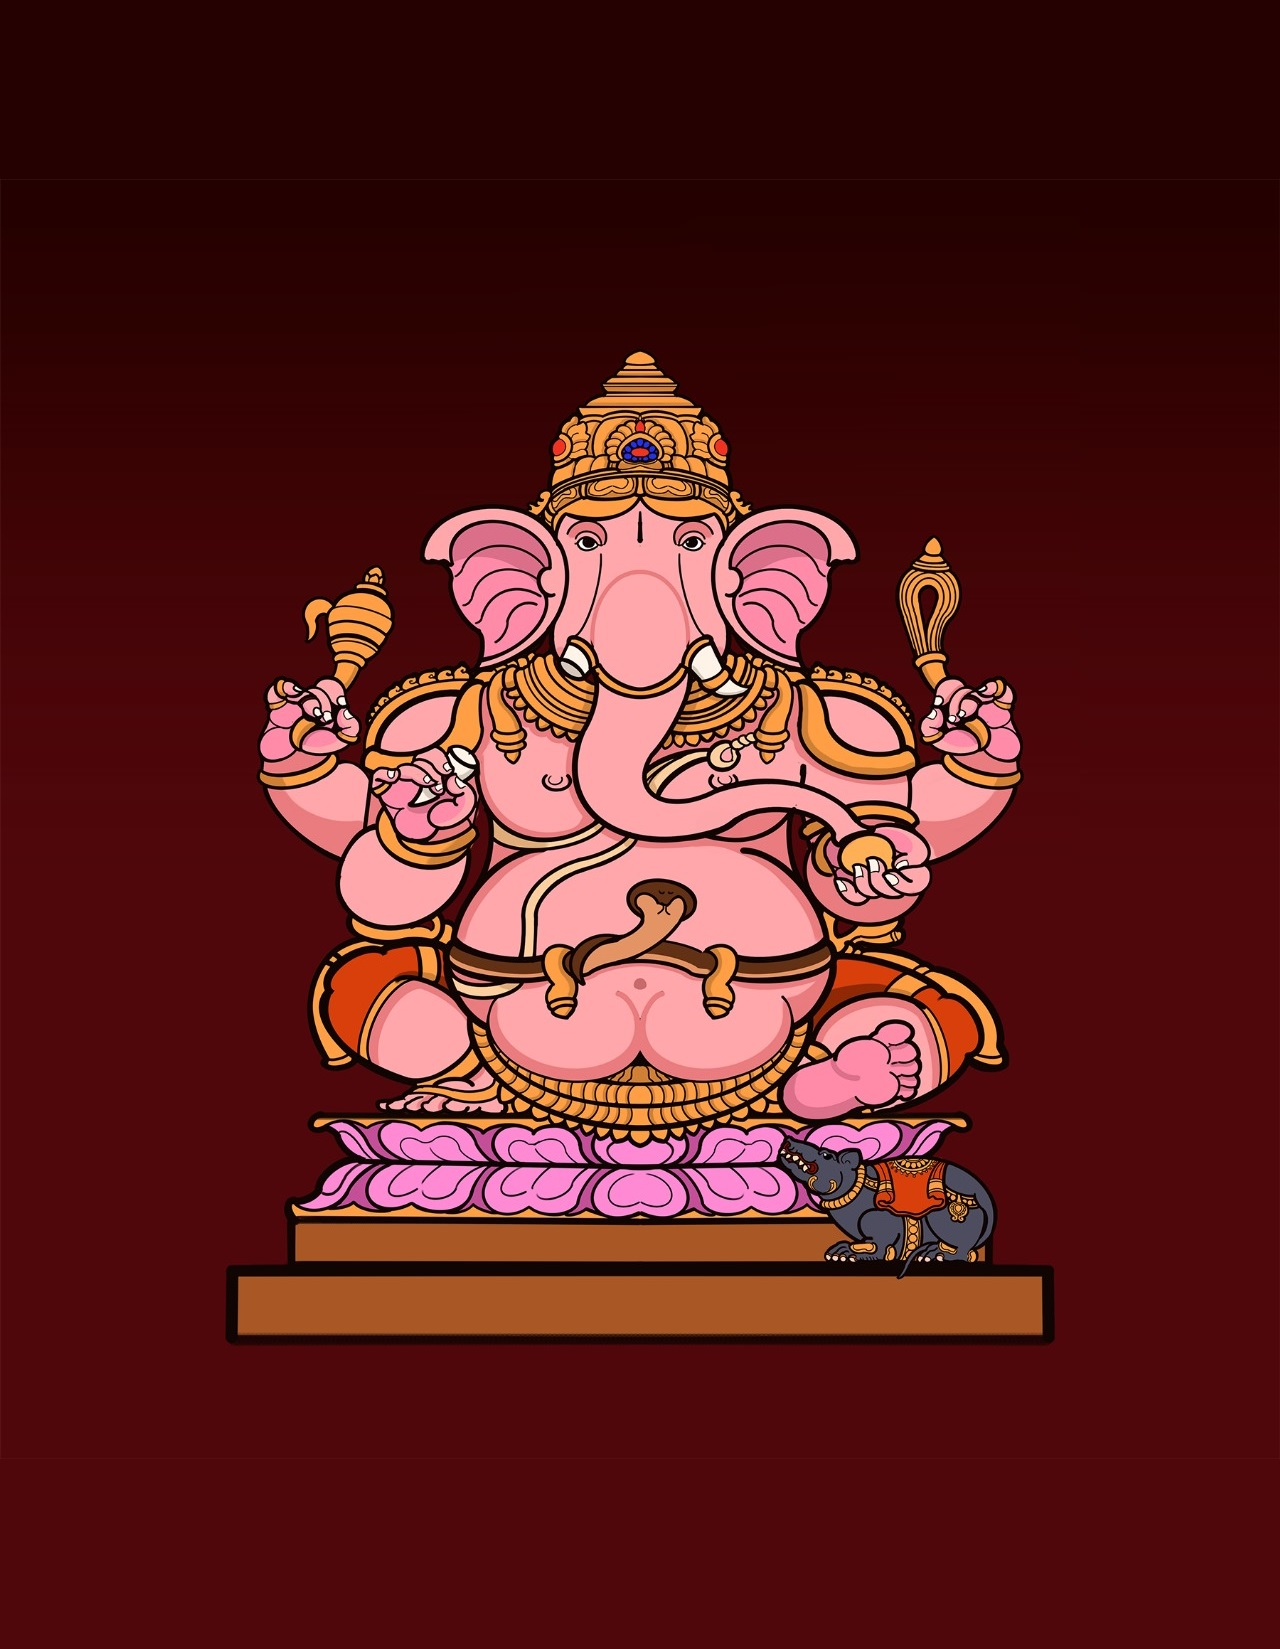
\includegraphics[width=0.9\textwidth, height=\paperheight, keepaspectratio]{./images/ganapa.jpg}
%\end{center}
%\restoregeometry % Restore original geometry settings
%\newpage

\clearpage
\newgeometry{margin=0pt} % Apply margin only for this page
\thispagestyle{empty}
%\begin{figure}
%\centering
%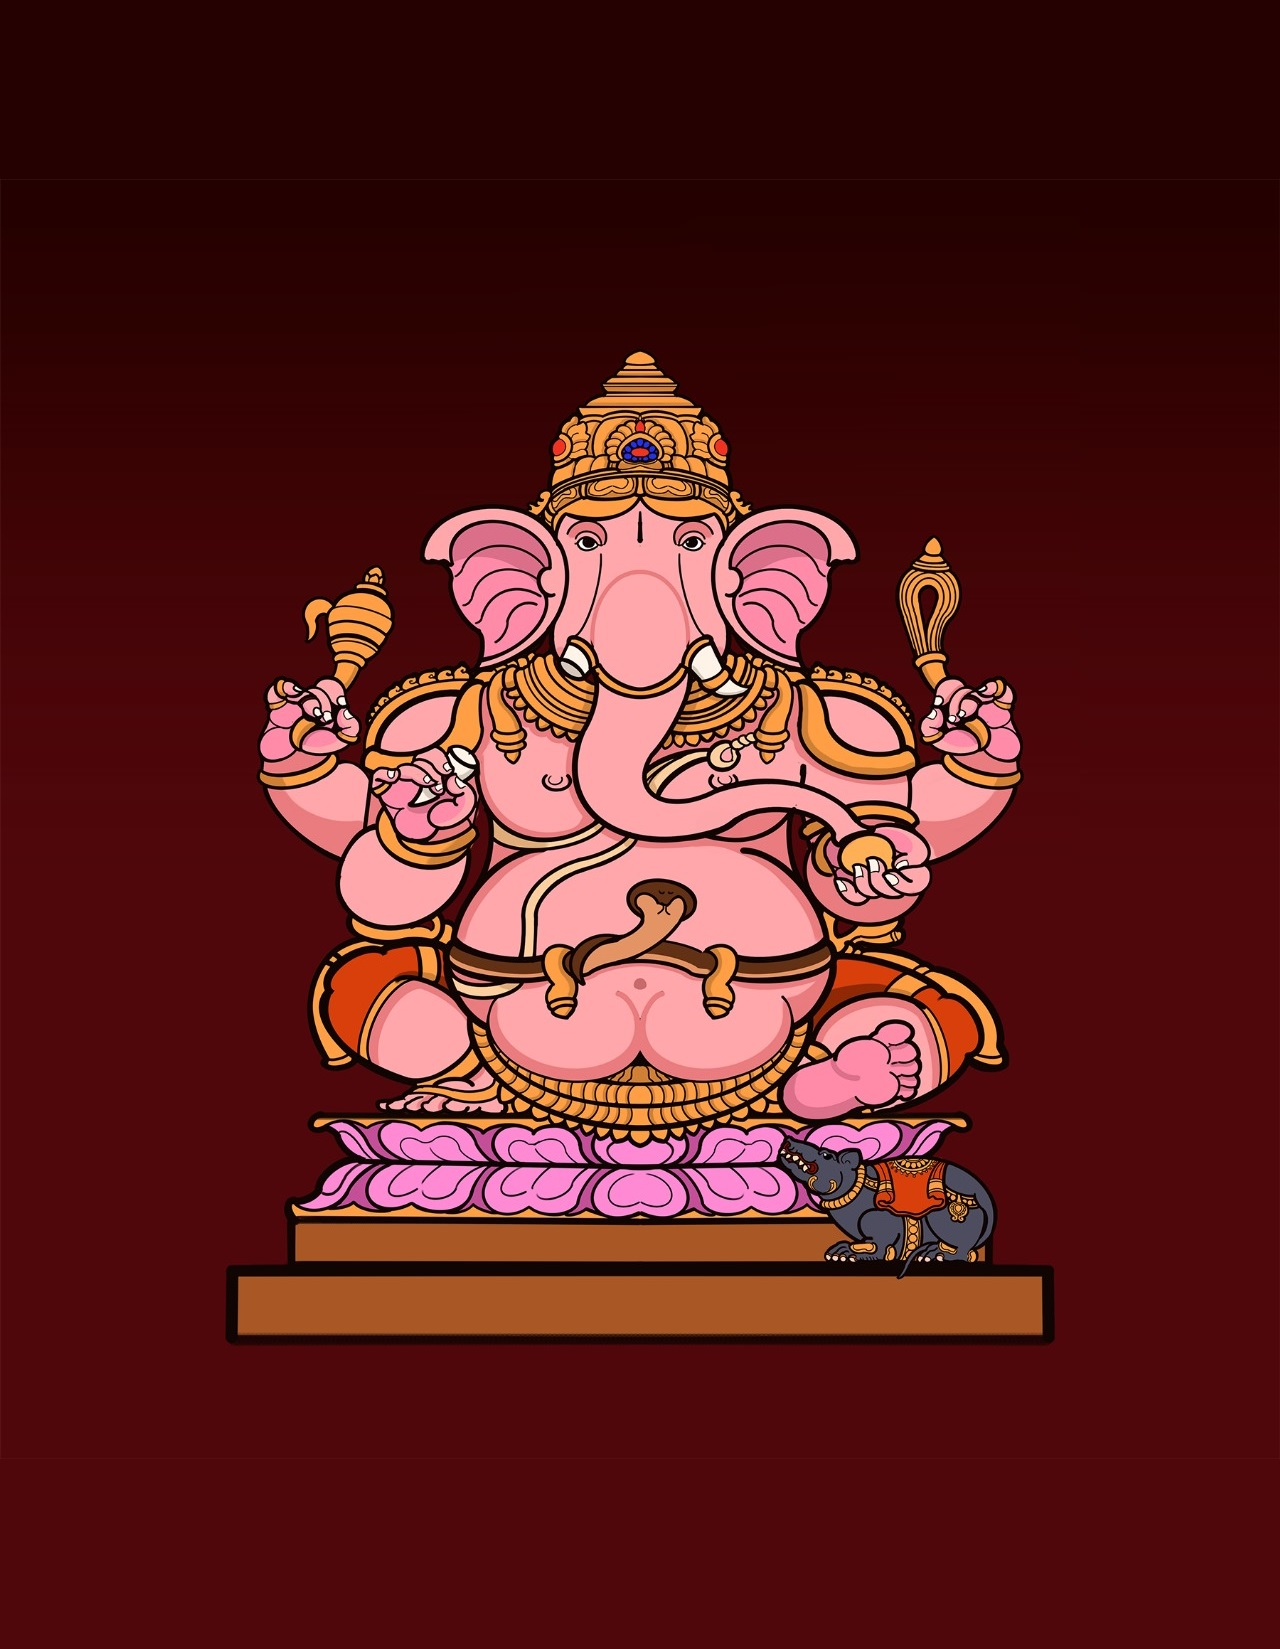
\includegraphics[width=0.9\textwidth, height=\paperheight, keepaspectratio]{./images/ganapa.jpg}
%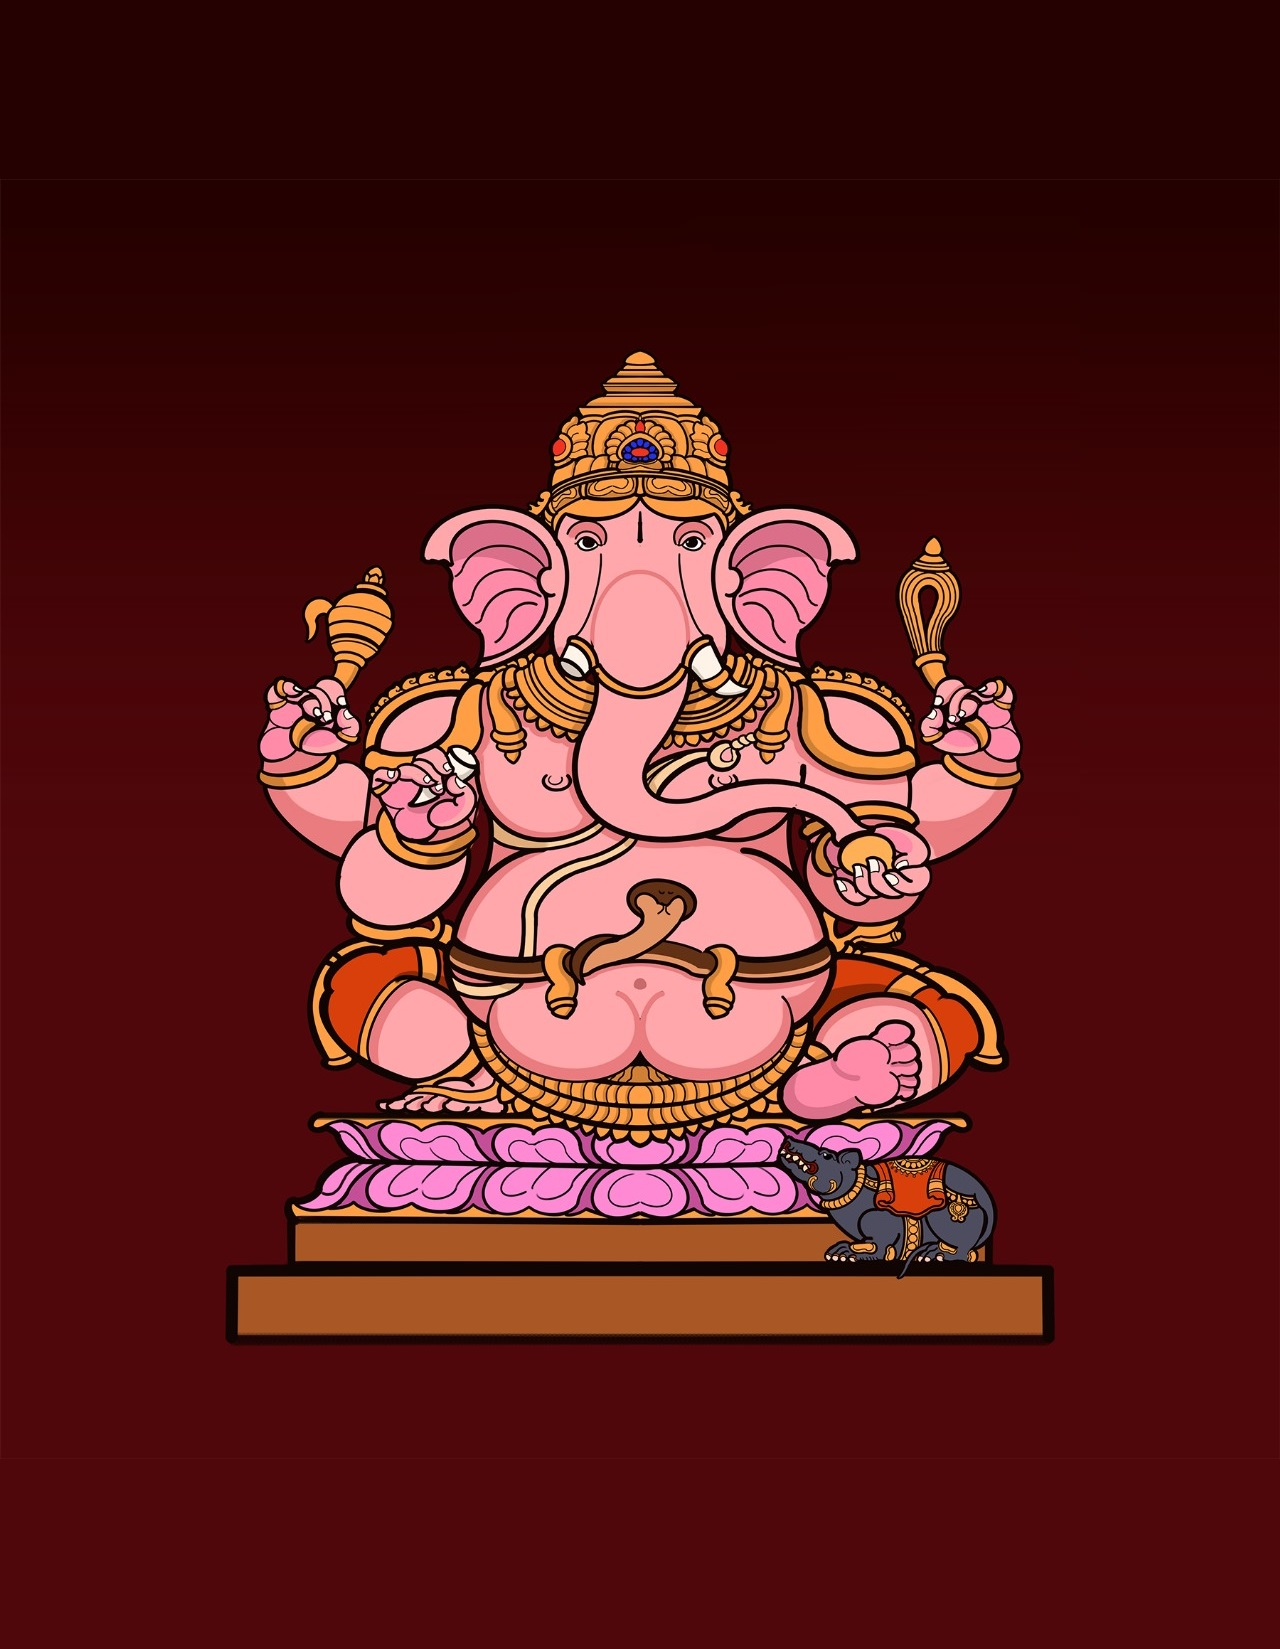
\includegraphics[width=\paperwidth, height=\paperheight]{./images/ganapa.jpg}
%\end{figure}
%\restoregeometry % Restore original geometry settings
%\newpage

\begin{figure}[h!]
    \centering
    \begin{overpic}[width=\paperwidth, height=\paperheight]{../images/001.jpg}
        \put(13,85){\color{white}\kanfont ಗಜಾನನಂ ಭೂತಗಣಾದಿ ಸೇವಿತಂ ಕಪಿತ್ಥ ಜಂಬೂಫಲಸಾರ ಭಕ್ಷಿತಮ್। }\put(10,82){\color{white}\kanfont ಉಮಾಸುತಂ ಶೋಕ ವಿನಾಶಕಾರಣಂ ನಮಾಮಿ ವಿಘ್ನೇಶ್ವರ ಪಾದಪಂಕಜಮ್॥ }
    \end{overpic}
    \caption{This is the standard figure caption below the image.}
    \label{fig:example}
\end{figure}

\restoregeometry

\thispagestyle{empty}
\thispagestyle{empty}
\pagestyle{fancy}


\chapter{\kanfont ಮುನ್ನುಡಿ}
\begin{center}
ದಿಶಂತು ಶಂ ಮೇ ಗುರುಪಾದಪಾಂಸವಃ ॥\\
\end{center}
\footnotesize \mananamtext{ಶ್ರಿ\!\char"0CD5ಮದ್ ಭಗವದ್ಗೀತೆಯು ಎಲ್ಲಾ ಧರ್ಮಗ್ರಂಥಗಳಲ್ಲಿ ಒಂದು ಅನನ್ಯ ಮತ್ತು ಸಾಟಿಯಿಲ್ಲದ ರತ್ನವಾಗಿದೆ.  ಇದು ಪರಿತ್ಯಾಗ ಮಾಡುವವರಿಗೆ ಮಾತ್ರವಲ್ಲದೆ ಲೌಕಿಕ ಜವಾಬ್ದಾರಿಗಳನ್ನು ಹೊತ್ತಿರುವವರಿಗೂ ಮಾರ್ಗದರ್ಶಿ ಬೆಳಕಾಗಿ ಕಾರ್ಯನಿರ್ವಹಿಸುತ್ತದೆ, ಆಧ್ಯಾತ್ಮಿಕದೊಂದಿಗೆ ಪ್ರಾಪಂಚಿಕತೆಯನ್ನು ಸಮತೋಲನಗೊಳಿಸಲು ಪ್ರಯತ್ನಿಸುತ್ತದೆ; ಇದು, ಅಜ್ಞಾನದಿಂದ ಅವರು (ಸಾಮಾನ್ಯ ಜನ) ತಮ್ಮನ್ನು ತಾವು,   ದೇಹ ಮತ್ತು ಮನಸ್ಸಿನ ವ್ಯವಹಾರಗಳ  ಜೊತೆ ಗುರುತಿಸಿಕೊಂಡಾಗ, ಅಂತಹ ವ್ಯವಹಾರಗಳ ಬಗ್ಗೆ ನಿಷ್ಪಕ್ಷಪಾತವಾಗಿರುವಂತೆ ಪ್ರತಿಪಾದಿಸುತ್ತದೆ.\\
ಜೀವನದಲ್ಲಿ ಒಬ್ಬರ ಕರ್ತವ್ಯಗಳನ್ನು ಸಾಧಿಸಲು, ಬಾಂಧವ್ಯದ ಅಥವಾ, ಮೋಹದ ಭಾವನೆ ಇರಬೇಕು ಎಂಬುದು ಒಂದು ತಪ್ಪು ಕಲ್ಪನೆ.  ಭಗವಾನ್ ಕೃಷ್ಣ, ಎಲ್ಲರಿಗಿಂತಲೂ  ದೊಡ್ಡ ಸಂಸಾರಿ ಹಾಗೂ, ಪರಿಪೂರ್ಣವಾದ ಮೋಹರಹಿತನಾದ ಅಸಂಸಾರಿ; ದಿವ್ಯವಾದ ಆನಂದದಲ್ಲಿ ನೆಲೆಗೊಂಡು, ಈ ಮೂರ್ತ, ಭೌತಿಕ ಜಗತ್ತಿನಲ್ಲಿ ಹೇಗೆ ಕಾರ್ಯನಿರ್ವಹಿಸಬೇಕು ಎಂಬುದನ್ನು ಅವನು ತನ್ನ ಕಾರ್ಯಗಳು, ಭಾವ ಮತ್ತು ಅವನು ಉಚ್ಛರಿಸುವ ಪ್ರತಿಯೊಂದೂ ಪರಮಪದದ  ಮೂಲಕ ಪ್ರದರ್ಶಿಸುತ್ತಾನೆ. ಆರಂಭದಲ್ಲಿ ‘ಸಂಘರ್ಷ ಮತ್ತು ಸವಾಲುಗಳಿಂದ ತುಂಬಿರುವ ಮಾರ್ಗ’ ಎಂದು ಕಂಡುಬoದರೂ ಸಹ, ಈ ಸ್ಥಿತಿಯನ್ನು ಸಾಧಿಸಲು (ದಿವ್ಯವಾದ ಆನಂದದಲ್ಲಿ ನೆಲೆಗೊಂಡು, ಈ ಮೂರ್ತ, ಭೌತಿಕ ಜಗತ್ತಿನಲ್ಲಿ  ಕಾರ್ಯನಿರ್ವಹಿಸುವುದು) ಸಮರ್ಥ ಶಿಕ್ಷಕರಿಂದ ಸರಿಯಾದ ಮಾರ್ಗದರ್ಶನದ ಅಗತ್ಯವಿದೆ. \\
ಈ ‘ನಿಪುಣ ಮಾರ್ಗದರ್ಶಿ ಕೈಪಿಡಿ’ಯಲ್ಲಿ, ಲೇಖಕರ ಆಳವಾದ ಒಳನೋಟದಿಂದ ಅಧ್ಯಾಯ 2 ರ 52-53 ಪದ್ಯಗಳಲ್ಲಿ ಸೂಚಿಸಿದಂತೆ: “ಶಿಕ್ಷಕರ ಮತ್ತು ಧರ್ಮಗ್ರಂಥಗಳ ಉದ್ದೇಶವು ನಮ್ಮನ್ನು ಭ್ರಮೆಯಿಂದ ಜಗ್ಗಿಸಿ, ಮುಕ್ತರನ್ನಾಗಿ ಮಾಡುವುದೇ ಆಗಿದೆ. ನಾವು ನಮ್ಮ ಲೌಕಿಕ ಚಿಂತನೆಯ ಮಾದರಿಗಳನ್ನು ಬಿಟ್ಟು, ಒಂದು ಉನ್ನತ ಸತ್ಯದಲ್ಲಿ (ಪಾರಮಾರ್ಥಿಕದಲ್ಲಿ) ಆಶ್ರಯ ಪಡೆಯಲು ಪ್ರಾರಂಭಿಸುತ್ತಿದ್ದಂತೆಯೇ, ಆಧ್ಯಾತ್ಮಿಕ ಪ್ರಯಾಣದ ಒಂದು ಭಾಗವಾದ ಗೊಂದಲಗಳು ಮತ್ತು ಸವಾಲುಗಳು ಏಳುತ್ತವೆ; ಆದರೆ, ನಾವು ಹೀಗೆ ಈ ಹಾದಿಯಲ್ಲಿ ಪ್ರಗತಿ ಹೊಂದುತ್ತಿದ್ದಂತೆ, ಸ್ಪಷ್ಟತೆ ಪಡೆಯಲು ಪ್ರಾರಂಭಿಸುತ್ತೇವೆ”.\\
ಈ ಪುಸ್ತಕವು ಲೇಖಕರ ಕ್ರಾಂತಿಕಾರಿ ಚಿಂತನೆಗಳ ಮೂಲಕ ಓದುಗರನ್ನು ದೇಹದಿಂದ, ಮನಸ್ಸಿಗೆ ಮತ್ತು ಮನಸ್ಸಿನಿಂದ ಪ್ರಜ್ಞೆಗೆ (ಚೈತನ್ಯಕ್ಕೆ), ಒಬ್ಬರ ಅಸ್ತಿತ್ವದ ಪದರಗಳನ್ನು ಭೇದಿಸುವಂತೆ ಮಾಡುತ್ತದೆ. \\
ಪ್ರತಿ ವಿಭಾಗದಲ್ಲಿ, ‘ಮನನಂ’ ಶೀರ್ಷಿಕೆಯಡಿಯಲ್ಲಿರುವ ಆತ್ಮಾವಲೋಕನದ ಪ್ರಶ್ನೆಗಳು, ಸ್ವಯಂ ಸಮಾಧಾನ ಮತ್ತು ಆತ್ಮವಂಚನೆಯಲ್ಲಿ (ಆತ್ಮ ಪ್ರವಂಚನ) ತೊಡಗಿರುವವರಿಗೆ ಯಾವುದೇ ವಿರಾಮ ನೀಡುವುದಿಲ್ಲ ಮತ್ತು ಪ್ರಾಮಾಣಿಕವಾದ ಸ್ವಯಂ ಮೌಲ್ಯಮಾಪನ ಮಾಡಲು ಅವರಿಗೆ ಸವಾಲು ಒಡ್ಡುತ್ತವೆ .  ಮತ್ತೊಂದೆಡೆ, ‘ಸ್ಫೂರ್ತಿ’ಯ ಅಡಿಯಲ್ಲಿರುವ ಪದಗಳು, ಪ್ರಯಾಸಕರ ಮತ್ತು ಗೊಂದಲಮಯ ಆಧ್ಯಾತ್ಮಿಕ ಮಾರ್ಗವನ್ನು ತುಲನಾತ್ಮಕವಾಗಿ ಸುಲಭಗೊಳಿಸಿ, ಸಕಾರಾತ್ಮಕತೆಯ ಒಂದು, ಅಕ್ಷಯವಾದ ಮೂಲವಾಗಿ ಕಾರ್ಯನಿರ್ವಹಿಸುತ್ತವೆ.\\
ಈ ಕೈಪಿಡಿಯು, ಆಕಾಂಕ್ಷಿಗಳಿಗೆ ಜೀವನದ ವಿವಿಧ ಸಮಸ್ಯೆಗಳಿಗೆ ಪರಿಹಾರವನ್ನು ಕಂಡುಕೊಳ್ಳಲು ಸಾಕಷ್ಟು ಸಮಾಧಾನಗಳನ್ನು  ನೀಡುತ್ತದೆ, ಆದರೆ ಬಾಹ್ಯವಾಗಿ ಅಲ್ಲ, ಆಂತರಿಕವಾಗಿ.\\
ಈ ಪುಸ್ತಕದ ವಿಷಯವು, ‘ಮಾನವ ಮನೋವಿಜ್ಞಾನ’ದ ಬಗ್ಗೆ ಲೇಖಕರ ಆಳವಾದ ತಿಳುವಳಿಕೆಯನ್ನು ತೋರಿಸುತ್ತದೆ, ಮೊದಲು ಸಕಾರಾತ್ಮಕ ಮಾನಸಿಕ ಸ್ಥಿತಿಯ ಕಡೆಗೆ ಮತ್ತು ನಂತರ ಅದನ್ನು ಮೀರಿ, ಆಂತರಿಕ ಶಾಶ್ವತವಾದ ಆತ್ಮದೆಡೆಗೆ, ಸರಳವಾಗಿ ಮುಂದುವರಿಯುತ್ತದೆ. \\
ಈ ಪುಸ್ತಕದ ಓದುಗರು ಈ ಪ್ರಯಾಣವನ್ನು ಪ್ರಾರಂಭಿಸಿದಾಗ, ಅವರು ಖಂಡಿತವಾಗಿಯೂ ಮಾನವ ಮನಸ್ಸಿನ ಕ್ಷೇತ್ರವನ್ನು ಮೀರುತ್ತಾರೆ ಮತ್ತು ಈ ಸ್ವರ್ಗೀಯ ಗೀತೆಯಾದ  ‘ಭಗವದ್ಗೀತೆ’ ಗಾಯಕನ ಕೃಪೆಯಿಂದ ‘ಅಧಿಷ್ಠಾನ ಚೈತನ್ಯಮ್’ (ಚೇತನಾತ್ಮಕದ ಅಂತಿಮ ಮೂಲತತ್ವ) ಅನ್ನು ತಲುಪುತ್ತಾರೆ. ಸಾಧಕರ ಅನುಕೂಲಕ್ಕಾಗಿ ತಮ್ಮ ಅಮೂಲ್ಯವಾದ ಆಲೋಚನೆಗಳನ್ನು ಲೇಖಿಸಿದ, ಸ್ವಾಮಿ ನಿರ್ಗುಣಾನಂದ ಗಿರಿ, ಇವರ ನಿಸ್ವಾರ್ಥ ಪ್ರಯತ್ನವನ್ನು,  ಸನಾತನ ಗುರುವಾದ, ಆ ಭಗವಂತ ಶ್ರೀಕೃಷ್ಣನು ಆಶೀರ್ವದಿಸಲಿ.\\\\
\begin{center}
ಮಂಗಳಂ ಸರ್ವಂ
\end{center}

{\kanBold ಸ್ವಾಮಿ ಸ್ವಾನಂದ ತೀರ್ಥ} \\
ಆಚಾರ್ಯ, ಕೈಲಾಸ್ ಆಶ್ರಮ\\
ಋಷಿಕೇಶ – ಉತ್ತರಖಂಡ\\
}
%\thispagestyle{empty}
\begin{onehalfspace}
\chapter{\kanfont ಪ್ರಸ್ತಾವನೆ}
\mananamtext{\indent ನಾವೆಲ್ಲರೂ ಜೀವನದ ಹೋರಾಟಗಳನ್ನು ಎದುರಿಸಲೇಬೇಕು. ಕುರುಕ್ಷೇತ್ರ ಯುದ್ಧದಲ್ಲಿ ಶ್ರೀ ಕೃಷ್ಣ ಪರಮಾತ್ಮನು, ತನ್ನ ವೇದನಾಯುಕ್ತ ಶಿಷ್ಯ ಅರ್ಜುನನಿಗೆ, ಪ್ರಾಪಂಚಿಕತೆಯಲ್ಲಿಯೂ ಅಧ್ಯಾತ್ಮಿಕತೆಯನ್ನು ಆಚರಣೆಗೆ ತರುವಂತಹ , ಸಂಕ್ಷಿಪ್ತ ಹಾಗೂ ಪ್ರಾಯೋಗಿಕವಾದ,  ಅತೀ ಪವಿತ್ರವಾದ ಬೋಧನೆಗಳನ್ನು ಕೊಟ್ಟಿದ್ದಾನೆ. ಈ ಶ್ರೇಷ್ಠವಾದ ಉಪನಿಷತ್ತುಗಳ ಸತ್ವಗಳನ್ನೊಳಗೊಂಡ  ಬೋಧನೆಗಳನ್ನು ಪವಿತ್ರವಾದ, ‘ಭಗವದ್ಗೀತ, ಒಂದು ಪವಿತ್ರ ಗಾನ’ ದ ಸ್ವರೂಪದಲ್ಲಿ, ಋಷಿ ವೇದವ್ಯಾಸರು ನಮಗೆ ನೀಡಿರುವ ಅಸೀಮವಾದ ಕೊಡುಗೆ. \\\\
\emph{ಅರ್ಜುನನು ಇದ್ದ ಪರಿಸ್ಥಿತಿಗೂ, ನಾವು ಇರುವ ಪರಿಸ್ಥಿತಿ ಮತ್ತು ಸಂಘರ್ಷಗಳಿಗೂ ವ್ಯತ್ಯಾಸಗಳಿರಬಹುದು. ಆದರೆ, ಗೀತೆಯ ಸಾರ್ವತ್ರಿಕ ಉಪದೇಶಗಳು ಸತ್ಯಾನ್ವೇಷಣೆ ಮಾಡಲು ಬಯಸುವ ಪ್ರಯೊಬ್ಬನಿಗೂ ಆತ್ಮೋನ್ನತಿ  ಮತ್ತು ಅಧ್ಯಾತ್ಮಿಕ ಪ್ರಗತಿ ಸಾಧಿಸಲು ಬೇಕಾಗುವ ಮಾದರಿಯಾಗಿದೆ.\\\\}
ಭಗವದ್ಗೀತೆಯ ಉಪದೇಶಗಳು ಕೇವಲ ಆಧ್ಯಾತ್ಮಿಕ ಅನ್ವೇಷಣೆ ಮಾಡುವವರಿಗೆ ಸಮರ್ಪಿತವಾದದ್ದು ಮಾತ್ರವೇ ಅಲ್ಲ, ಜೀವನಕ್ಕೆ ಬೇಕಾಗುವ ಅತ್ಯಮೂಲ್ಯವಾದ ಕೈಪಿಡಿಯೂ ಆಗಿದೆ. ಯಾರು, ಕೆಲಸದಲ್ಲಿ ಮತ್ತು ಕೌಟುಂಬಿಕ ಜವಾಬ್ದಾರಿಗಳಲ್ಲಿ ಒತ್ತಡ ರಹಿತವಾಗಿ, ಸಮತೋಲನ ಮತ್ತು ಮಾನಸಿಕ ನೆಮ್ಮದಿ ಕಾಪಾಡಿಕೊಳ್ಳಲು  ಬಯಸುತ್ತಾರೋ ಅವರಿಗೆ ಈ ಬೋಧನೆಗಳು ಬಹಳ ಮಹತ್ವದ್ದಾಗಿರುತ್ತವೆ. \\\\
ಅನೇಕ ಗುರುಗಳು ಮತ್ತು ವಿದ್ವಾಂಸರು ಈಗಾಗಲೇ ಮಾಡಿರುವಂತೆ ಈ ದಿನಚರಿ ಪುಸ್ತಕ ಮತ್ತು ನಿಯತಕಾಲಿಕವು, ಗೀತೆಯ ಬೋಧನೆಗಳನ್ನು ತಿಳಿಸುವ ಪ್ರಯತ್ನ ಅಥವಾ ವ್ಯಾಖ್ಯಾನ ಕೊಡುವುದಾಗಿಲ್ಲ. ಈ ಗೀತಾ ಮನನವು, ಬೋಧನೆಗಳ ಚಿಂತನೆ ಮಾಡುವುದು ಮತ್ತು ಅದನ್ನು ನಮ್ಮ ಸ್ವಂತದ್ದನ್ನಾಗಿ ಅಂದರೆ, ಜೀವನದಲ್ಲಿ ಅಳವಡಿಸಿಕೊಳ್ಳಲು ಸುಲಭವಾಗುವಂತೆ ಮಾಡಿಕೊಳ್ಳುವುದೇ ಆಗಿದೆ. ದೇವ ನಾಗರಿಯಲ್ಲಿರುವ `ಮನನ` ಎಂಬ ಪದವು ಆಗಲೇ ಕೇಳಿದ್ದನ್ನು ಅಥವಾ ಓದಿದ್ದನ್ನು ಚಿಂತನೆ ಮಾಡುವ ಕಾರ್ಯವಿಧಾನವನ್ನು ಅನ್ವಯಿಸುವುದಾಗಿದೆ.\\\\
ಈ ದಿನಚರಿ ಪುಸ್ತಕವನ್ನು ನೀವು, ನಿಮ್ಮ ಮನಸ್ಸಿನ ಇಂಗಿತವನ್ನು ಸ್ವತಂತ್ರವಾಗಿ ವ್ಯಕ್ತಪಡಿಸಲು  ಮತ್ತು ನಿಮ್ಮ ಜೀವನದಲ್ಲಿ ಅಳವಡಿಸಿಕೊಳ್ಳಲು ಅವಕಾಶ ಮಾಡಿಕೊಡುವ ಸಲುವಾಗಿ  ರೂಪಿಸಲಾಗಿದೆ. ಗೀತೆಯಲ್ಲಿರುವ ಶ್ಲೋಕಗಳ ಆಧಾರದ ಮೇಲೆ ರಚಿಸಲಾಗಿರುವ ಈ ಪ್ರಶ್ನೆಗಳು, ಆಯಾ ಬೋಧನೆಗಳ ಸನ್ನಿವೇಶಕ್ಕೆ ತಕ್ಕಂತೆ, ನಿಮ್ಮ ವೈಯಕ್ತಿಕ ಅರ್ಥಗಳನ್ನು ಹುಡುಕಲು ಮತ್ತು ಅದರಿಂದ ಜೀವನದ ಸಂದರ್ಭದೊಳಗೆ ಅಪಾರ ಸ್ಪಷ್ಟನೆ ದೊರಕಿಸಲು ಸಹಾಯಕವಾಗುವಂತೆ ರೂಪಿಸಲಾಗಿದೆ.
ಶ್ರೀ ಕೃಷ್ಣ ಪರಮಾತ್ಮನು  ಅರ್ಜುನನಿಗೆ ಧಾರ್ಮಿಕ ಯುದ್ಧವನ್ನು ಮಾಡಲು ಪ್ರೇರೇಪಿಸಿದಂತೆ, ನಿಮ್ಮ ಜೀವನದ ದಿನನಿತ್ಯದ ಕರ್ತವ್ಯಗಳನ್ನು ಈ “ಗೀತಾ ಮನನಮ್ “ ಮೂಲಕ  ಸಮರ್ಪಕವಾಗಿ ನಿರ್ವಹಿಸಲು,  ಆ ಭಗವಂತ ನಿಮ್ಮನ್ನೂ ಪ್ರೇರೇಪಿಸುತ್ತಾನೆ ಎಂದು ನಂಬುತ್ತೇನೆ. ನಿಮ್ಮ ಅಂತರಂಗದ ಶಾಂತಿ, ವೈಯಕ್ತಿಕ ಪ್ರಗತಿಯನ್ನು ನಿರ್ಲಕ್ಷಿಸದೇ, ನಿಮ್ಮ ಕರ್ತವ್ಯಗಳನ್ನು ಕುಶಲತೆಯಿಂದ ಯಶಸ್ವಿಯಾಗಿ ನಿರ್ವಹಿಸುತ್ತಾ  ಮತ್ತು ನಿಶ್ಚಲವಾಗಿ ದೈವತ್ವದಲ್ಲಿ ಮನಸನ್ನಿಡುವುದೇ, ಈ ದಿವ್ಯವಾದ ಗೀತೆಯ ನಿರಂತರ ಉದ್ದೇಶ.\\\\
ನಾನು ಈ ಪುಸ್ತಕದಲ್ಲಿ ಬಳಸಿರುವ ಚಿತ್ರಕಲೆ ಮತ್ತು ರೇಖಾಚಿತ್ರಗಳಿಗಾಗಿ ------ ಅವರಿಗೆ ಧನ್ಯವಾದಗಳನ್ನು ಸಲ್ಲಿಸುತ್ತೇನೆ. ಮುದ್ರಣ ಕಾರ್ಯದಲ್ಲಿ ಸಹಾಯ ಮಾಡಿದ -----ಅವರಿಗೆ ನಾನು ಕೃತಜ್ಞತೆ ವ್ಯಕ್ತಪಡಿಸುತ್ತೇನೆ. ನನ್ನ ಗೀತಾ ತರಗತಿಯಲ್ಲಿ ಭಾಗವಹಿಸಿದ್ದ ಅನೇಕ ವಿದ್ಯಾರ್ಥಿಗಳು ಶ್ಲೋಕಗಳ ಭಾಷಾಂತರ, ತಿದ್ದುವಿಕೆ, ಸಂಪಾದನೆ, ವಿನ್ಯಾಸ ಮತ್ತು ಮುದ್ರಣ ಪ್ರಕ್ರಿಯೆಯನ್ನು ಗಮನಿಸುವಲ್ಲಿ ತೊಡಗಿಸಿಕೊಂಡಿದ್ದಾರೆ. ಈ ಗ್ರಂಥವನ್ನು ಓದುಗರ ಹಿತಾರ್ಥಕ್ಕಾಗಿ ಸಮರ್ಪಣೆಯಿಂದ ಮಾಡಿದ ಅವರ ತ್ಯಾಗಮಯ ಸೇವೆಗೆ ಭಗವಂತನ ಕೃಪೆ ಹಾಗು ನನ್ನ ಆಶೀರ್ವಾದಗಳು. }

\end{onehalfspace}
\mainmatter
\centerline{\textbf{ಅಥ ಪ್ರಥಮೋऽಧ್ಯಾಯಃ ।}\\}
ಮೊಟ್ಟ ಮೊದಲನೆಯ ಶ್ಲೋಕವೇ ನಮಗೆ ಚಿಂತನೆ, ಮನನ ಪ್ರಾರಂಭಿಸಲು ಬೇಕಾಗುವ ಸೂಕ್ಷ್ಮವಾದ ಸಂದೇಶವನ್ನು ಕೊಡುತ್ತದೆ.\\
\slcol{ಧೃತರಾಷ್ಟ್ರ ಉವಾಚ ।\\
\index{ಧರ್ಮಕ್ಷೇತ್ರೇ ಕುರುಕ್ಷೇತ್ರೇ} ಸಮವೇತಾ ಯುಯುತ್ಸವಃ ।\\
ಮಾಮಕಾಃ ಪಾಂಡವಾಶ್ಚೈವ ಕಿಮಕುರ್ವತ ಸಂಜಯ ॥ 1 ॥}
\cquote{ಧೃತರಾಷ್ಟ್ರನು ಹೇಳಿದನು,\\
ಸಂಜಯನೇ, ಯುದ್ಧದ ಬಯಕೆಯಿಂದ ಧರ್ಮಭೂಮಿಯಾದ ಕುರುಕ್ಷೇತ್ರದಲ್ಲಿ ಕಲೆತ ನನ್ನ ಮಕ್ಕಳೂ ಪಾಂಡವರೂ ಏನು ಮಾಡಿದರು?\\}
\slcol{ಸಂಜಯ ಉವಾಚ ।\\
\index{ದೃಷ್ಟ್ವಾ ತು ಪಾಂಡವಾನೀಕಂ} ವ್ಯೂಢಂ ದುರ್ಯೋಧನಸ್ತದಾ ।\\
ಆಚಾರ್ಯಮುಪಸಂಗಮ್ಯ ರಾಜಾ ವಚನಮಬ್ರವೀತ್ ॥ 2 ॥}
\cquote{ಸಂಜಯನು ಹೇಳಿದನು,\\
ಪಾಂಡವರ ದಂಡು ಸಜ್ಜಾಗಿ ನಿಂತಿದ್ದುದನ್ನು ನೋಡಿದ ಅರಸನಾದ ದುರ್ಯೋಧನನು ಗುರುಗಳಾದ ದ್ರೋಣರ ಬಳಿಗೆ ಬಂದು ಹೀಗೆ ಹೇಳಿದನು. \\}
\slcol{\index{ಪಶ್ಯೈತಾಂ ಪಾಂಡುಪುತ್ರಾಣಾಮಾಚಾರ್ಯ} ಮಹತೀಂ ಚಮೂಮ್ ।\\
ವ್ಯೂಢಾಂ ದ್ರುಪದಪುತ್ರೇಣ ತವ ಶಿಷ್ಯೇಣ ಧೀಮತಾ ॥ 3 ॥}
\cquote{ಗುರುಗಳೇ, ದೃಪದರಾಜನ ಮಗ ನಿಮ್ಮ ಶಿಷ್ಯ, ಬುದ್ಧಿಶಾಲಿಯಾದ ದೃಷ್ಟದ್ಯುಮ್ನ ಪಾಂಡವರ ಈ ದೊಡ್ಡ ದಂಡನ್ನು ಸಜ್ಜುಗೊಳಿಸಿರುವುದನ್ನು ನೋಡಿರಿ.\\}
\slcol{\index{ಅತ್ರ ಶೂರಾ ಮಹೇಷ್ವಾಸಾ} ಭೀಮಾರ್ಜುನಸಮಾ ಯುಧಿ ।\\
ಯುಯುಧಾನೋ ವಿರಾಟಶ್ಚ ದ್ರುಪದಶ್ಚ ಮಹಾರಥಃ ॥ 4 ॥}

\newpage
\begin{mananam}{\kanfont ಮನನ ಶ್ಲೋಕ - }
{\footnotesize \mananamfont ನನ್ನ ಜೀವನದ ದೈನಂದಿನ ನಿತ್ಯಕರ್ಮದಲ್ಲಿ ಯಾವಾಗ ನನ್ನ ದೇಹವು, ಆಸೆ, ಕೋಪ, ಭಯ, ಮತ್ಸರ ಇತ್ಯಾದಿಗಳಲ್ಲಿ ಒಲವು ತೋರುವುದನ್ನು ಗುರುತಿಸಿತು, ಅವುಗಳನ್ನು ಸ್ವಾತಂತ್ರ್ಯವನ್ನು ಆಳವಾಗಿ ಪ್ರೇರೇಪಿಸುವ ನನ್ನನ್ನು ಪ್ರತಿಭಟಿಸುವಂತೆ ಮಾಡುವ ಮತ್ತು ಸನಾತನ ಗ್ರಂಥ ಮತ್ತು ಬೋಧಕರಿಂದ ಪಡೆದ ಜ್ಞಾನವನ್ನು ಯಾವ ಬಲವನ್ನು ಅನುಸರಿಸಿದೆ? ನನ್ನ ಹಂಬಲ ಮತ್ತು ಸಂಕಲ್ಪಗಳನ್ನು ತಳ್ಳಿಹಾಕುವ ನನ್ನ ದುರಭ್ಯಾಸಗಳು ಮತ್ತು ಅಪಾಯಕಾರಿ ನಡವಳಿಕೆಗಳಿಂದಾಗಿ ನನ್ನ ನಿತ್ಯ ಜೀವನದಲ್ಲಿ ಏನೇನು ಕಷ್ಟ ಪಡಬೇಕಾಯಿತು?}
\end{mananam}
\WritingHand\enspace\textbf{ಆತ್ಮ ವಿಮರ್ಶೆ}
\begin{inspiration}{\kanfont ಸ್ಪೂರ್ತಿ}
{\footnotesize \mananamfont ನಿನಗೆ ನೀನು ಸತ್ಯವಾಗಿರು ಮತ್ತು ನೀನು ಉನ್ನತಿಯತ್ತ ಬದಲಾಗುವೆ. ಜೀವನದಲ್ಲಿ ಜಾಣನಿಗೆ ಅವಶ್ಯಕವಾದುದು ಪಕ್ಷಪಾತ ರಹಿತ ಅವಲೋಕನ. ನಮ್ಮನ್ನು ನಾವು ಬದಲಾಯಿಸಿಕೊಳ್ಳಲು ಕೇವಲ ಬಯಕೆ ಇದ್ದರೆ ಮಾತ್ರ ಸಾಲದು. ಜ್ಞಾನಿಗಳ ಮಹತ್ವದ, ಉನ್ನತವಾದ ಬೋಧನೆಗಳಿಂದ ನಮ್ಮ ಯೋಚನೆಗಳು, ಮಾತುಗಳು ಮತ್ತು ಕೃತಿಗಳನ್ನು ತಹಬಂದಿಗೆ ತಂದು, ಪ್ರತಿದಿನವೂ ನಮ್ಮನ್ನು ನಾವು ಆತ್ಮ ವಿಮರ್ಶೆ ಮಾಡಿಕೊಳ್ಳಲೇಬೇಕು.}
\end{inspiration}
\newpage

\cquote{ಈ ದಂಡಿನಲ್ಲಿ ಹೋರಾಟದಲ್ಲಿ ಭೀಮಾರ್ಜುನರಿಗೆ ಸರಿ ಜೋಡಿಯಾದ ಶೂರರಾಗಿ ದೊಡ್ಡ ದೊಡ್ಡ ಬಿಲ್ಲುಗಳನ್ನು ಹಿಡಿದುಕೊಂಡು ಕಾದುವುದರಲ್ಲಿ ಕುಶಲರಾದ ಸಾತ್ಯಕಿ ವಿರಾಟರಿದ್ದಾರೆ. ಸಹಸ್ರ ಜನರೊಡನೆ ಏಕಾಂಗಿಯಾಗಿ ಹೋರಾಡಬಲ್ಲ ದ್ರುಪದನಿದ್ದಾನೆ.\\}
\slcol{\index{ಧೃಷ್ಟಕೇತುಶ್ಚೇಕಿತಾನಃ} ಕಾಶಿರಾಜಶ್ಚ ವೀರ್ಯವಾನ್ ।\\
ಪುರುಜಿತ್ಕುಂತಿಭೋಜಶ್ಚ ಶೈಬ್ಯಶ್ಚ ನರಪುಂಗವಃ ॥ 5 ॥}
\cquote{ದೃಷ್ಟಕೇತು, ಚೀಕಿತಾನ, ವೀರನಾದ ಕಾಶಿರಾಜ, ಮತ್ತು ಮನುಷ್ಯರಲ್ಲಿ ಶ್ರೇಷ್ಠನಾದ ಶೈಭ್ಯ ಇವರೆಲ್ಲ ಇದ್ದಾರೆ. \\} 
\slcol{\index{ಯುಧಾಮನ್ಯುಶ್ಚ ವಿಕ್ರಾಂತ} ಉತ್ತಮೌಜಾಶ್ಚ ವೀರ್ಯವಾನ್ ।\\
ಸೌಭದ್ರೋ ದ್ರೌಪದೇಯಾಶ್ಚ ಸರ್ವ ಏವ ಮಹಾರಥಾಃ ॥ 6 ॥}
\cquote{ಬಲಶಾಲಿಯಾದ ಯುಧಾಮನ್ಯು, ವೀರನಾದ ಉತ್ತಮೌಜ, ಸುಭದ್ರೆಯ ಮಗ ಅಭಿಮನ್ಯು ಮತ್ತು ದ್ರೌಪದಿಯ ಮಕ್ಕಳು ಇದ್ದಾರೆ. ಎಲ್ಲರೂ ಒಬ್ಬೊಬ್ಬರು ಹತ್ತು ಸಹಸ್ರ ಜನರೊಡನೆ ಹೋರಾಡಬಲ್ಲ ಮಹಾರುತರು. \\}
\slcol{\index{ಅಸ್ಮಾಕಂ ತು ವಿಶಿಷ್ಟಾ ಯೇ} ತಾನ್ನಿಬೋಧ ದ್ವಿಜೋತ್ತಮ ।\\
ನಾಯಕಾ ಮಮ ಸೈನ್ಯಸ್ಯ ಸಂಙ್ಞಾರ್ಥಂ ತಾನ್ಬ್ರವೀಮಿ ತೇ ॥ 7 ॥}
\cquote{ಬ್ರಾಹ್ಮಣ ಶ್ರೇಷ್ಠರೇ, ನಮ್ಮ ಕಡೆಯಲ್ಲಿರುವ ವೀರರನ್ನು ನೆನಪಿಗೆ ತಂದುಕೊಳ್ಳಿ. ತಮಗೆ ನೆನಪಾಗಲೆಂದು ಅವರ ಹೆಸರುಗಳನ್ನು ಹೇಳುತ್ತೇನೆ.\\} 
\slcol{\index{ಭವಾನ್ಭೀಷ್ಮಶ್ಚ ಕರ್ಣಶ್ಚ} ಕೃಪಶ್ಚ ಸಮಿತಿಂಜಯಃ ।\\
ಅಶ್ವತ್ಥಾಮಾ ವಿಕರ್ಣಶ್ಚ ಸೌಮದತ್ತಿಸ್ತಥೈವ ಚ ॥ 8 ॥}
\cquote{ತಾವು ಭೀಷ್ಮ ಕರ್ಣ ಜಯಶೀಲನಾದ ಕೃಪಾ, ಅಶ್ವತ್ಥಾಮ, ವಿಕರ್ಣ ಸೋಮದತ್ತನ ಮಗನಾದ ಭೂರಿಶ್ರವ ಮತ್ತು ಜಯದ್ರಥ. \\}
\slcol{\index{ಅನ್ಯೇ ಚ ಬಹವಃ} ಶೂರಾ ಮದರ್ಥೇ ತ್ಯಕ್ತಜೀವಿತಾಃ ।\\
ನಾನಾಶಸ್ತ್ರಪ್ರಹರಣಾಃ ಸರ್ವೇ ಯುದ್ಧವಿಶಾರದಾಃ ॥ 9 ॥}
\cquote{ಇನ್ನೂ ಅನೇಕ ಶೂರರು ನನಗಾಗಿ ಜೀವ ತೆರಲು ಸಿದ್ದರಾಗಿ ಇದ್ದಾರೆ. ಎಲ್ಲರೂ ಎಲ್ಲ ಬಗಯ ಆಯುಧಗಳನ್ನು ಉಪಯೋಗಿಸಬಲ್ಲವರು ಮತ್ತು ಯುದ್ಧದಲ್ಲಿ ಗಟ್ಟಿಗರು.\\}
\slcol{\index{ಅಪರ್ಯಾಪ್ತಂ ತದಸ್ಮಾಕಂ} ಬಲಂ ಭೀಷ್ಮಾಭಿರಕ್ಷಿತಮ್ ।\\
ಪರ್ಯಾಪ್ತಂ ತ್ವಿದಮೇತೇಷಾಂ ಬಲಂ ಭೀಮಾಭಿರಕ್ಷಿತಮ್ ॥ 10 ॥}
\cquote{ಭೀಷ್ಮರ ರಕ್ಷಣೆಗೆ ಒಳಪಟ್ಟಿರುವ ನಮ್ಮ ದೊಡ್ಡ ಆ ದಂಡು ಸಾಲದೇನೋ ಎನಿಸುತ್ತದೆ. ಭೀಮನ ರಕ್ಷಣೆಗೆ ಒಳಪಟ್ಟಿರುವ ಪಾಂಡವರ ಈ ಸೇನೆ ಸಾಕಷ್ಟು ಸಮರ್ಥವಾಗಿದೆ.\\}
\slcol{\index{ಅಯನೇಷು ಚ ಸರ್ವೇಷು} ಯಥಾಭಾಗಮವಸ್ಥಿತಾಃ ।\\
ಭೀಷ್ಮಮೇವಾಭಿರಕ್ಷಂತು ಭವಂತಃ ಸರ್ವ ಏವ ಹಿ ॥ 11 ॥}
\cquote{ನೀವೆಲ್ಲರೂ ದಂಡಿನ ಬೇರೆ ಬೇರೆ ಮಾರ್ಗಗಳಲ್ಲಿ ನಿಮ್ಮ ನಿಮ್ಮ ಪಾಲಿಗೆ ಬಂದ ಕಡೆ ಇದ್ದುಕೊಂಡು ಭೀಷ್ಮನನ್ನು ರಕ್ಷಿಸಿರಿ.\\}
\slcol{\index{ತಸ್ಯ ಸಂಜನಯನ್ಹರ್ಷಂ} ಕುರುವೃದ್ಧಃ ಪಿತಾಮಹಃ ।\\
ಸಿಂಹನಾದಂ ವಿನದ್ಯೋಚ್ಚೈಃ ಶಂಖಂ ದಧ್ಮೌ ಪ್ರತಾಪವಾನ್ ॥ 12 ॥}
\cquote{ಹೀಗೆಂದು ಹೇಳಿದ ದುರ್ಯೋಧನನಿಗೆ ಹರ್ಷ ಉಂಟಾಗುವಂತೆ ಆಗ ಕುರುವಂಶದ ಹಿರಿಯ ಕೌರವರ ಅಜ್ಜ, ಪರಾಕ್ರಮಶಾಲಿ ಭೀಷ್ಮನು ಗಟ್ಟಿಯಾಗಿ ಸಿಂಹನಾದ ಮಾಡಿ ಶಂಖವನ್ನು ಊದಿದನು.\\}
\slcol{\index{ತತಃ ಶಂಖಾಶ್ಚ ಭೇರ್ಯಶ್ಚ} ಪಣವಾನಕಗೋಮುಖಾಃ ।\\
ಸಹಸೈವಾಭ್ಯಹನ್ಯಂತ ಸ ಶಬ್ದಸ್ತುಮುಲೋऽಭವತ್ ॥ 13 ॥}
\cquote{ಆಮೇಲೆ ಒಮ್ಮೆಲೆ ಶಂಖಗಳು, ಭೇರಿಗಳು, ಮೃದಂಗಗಳು, ನಗಾಡಿಗಳು, ರಣ ಸಿಂಹಗಳು ಒಳಗಿದವು. ಆ ಗದ್ದಲವು ಎಲ್ಲೆಲ್ಲಿಯೂ ತುಂಬಿತು.\\}
\slcol{\index{ತತಃ ಶ್ವೇತೈರ್ಹಯೈರ್ಯುಕ್ತೇ} ಮಹತಿ ಸ್ಯಂದನೇ ಸ್ಥಿತೌ ।\\
ಮಾಧವಃ ಪಾಂಡವಶ್ಚೈವ ದಿವ್ಯೌ ಶಂಖೌ ಪ್ರದಘ್ಮತುಃ ॥ 14 ॥}
\cquote{ಆಮೇಲೆ ಬಿಳಿ ಕುದುರೆಯನ್ನು ಹೂಡಿದ ದೊಡ್ಡ ತೇರಿನ ಮೇಲೆ ಕುಳಿತಿದ್ದ ಕೃಷ್ಣನೂ ಅರ್ಜುನನೂ ಹೆಸರುವಾಸಿಯಾದ ದಿವ್ಯವಾದ ತಮ್ಮ ಶಂಖಗಳನ್ನು ಊದಿದರು.\\}
\slcol{\index{ಪಾಂಚಜನ್ಯಂ ಹೃಷೀಕೇಶೋ} ದೇವದತ್ತಂ ಧನಂಜಯಃ ।\\
ಪೌಂಡ್ರಂ ದಧ್ಮೌ ಮಹಾಶಂಖಂ ಭೀಮಕರ್ಮಾ ವೃಕೋದರಃ ॥ 15 ॥}
\cquote{ಕೃಷ್ಣನು ಪಾಂಚಜನ್ಯವನ್ನೂ ಅರ್ಜುನನ್ನು ದೇವದತ್ತವನ್ನೂ, ಶತ್ರುಗಳನ್ನು ಎದೆಗೂಡಿಸುವ ಭೀಮನು ಪೌಂಡ್ರವೆಂಬ ದೊಡ್ಡ ಶಂಖವನ್ನು ಓದಿದನು.\\}
\slcol{\index{ಅನಂತವಿಜಯಂ ರಾಜಾ} ಕುಂತೀಪುತ್ರೋ ಯುಧಿಷ್ಠಿರಃ ।\\
ನಕುಲಃ ಸಹದೇವಶ್ಚ ಸುಘೋಷಮಣಿಪುಷ್ಪಕೌ ॥ 16 ॥}
\cquote{ಕುಂತಿಯ ಹಿರಿಯ ಮಗ, ಅರಸನಾದ ಧರ್ಮರಾಯನು ಅನಂತ ವಿಜಯವನ್ನೂ ನಕುಲನೂ ಸುಘೋಷವನ್ನೂ ಸಹದೇವನು ಮಣಿಪುಷ್ಪಕವನ್ನೂ ಊದಿದರು. \\}
\slcol{\index{ಕಾಶ್ಯಶ್ಚ ಪರಮೇಷ್ವಾಸಃ} ಶಿಖಂಡೀ ಚ ಮಹಾರಥಃ ।\\
ಧೃಷ್ಟದ್ಯುಮ್ನೋ ವಿರಾಟಶ್ಚ ಸಾತ್ಯಕಿಶ್ಚಾಪರಾಜಿತಃ ॥ 17 ॥\\
\index{ದ್ರುಪದೋ ದ್ರೌಪದೇಯಾಶ್ಚ} ಸರ್ವಶಃ ಪೃಥಿವೀಪತೇ ।\\
ಸೌಭದ್ರಶ್ಚ ಮಹಾಬಾಹುಃ ಶಂಖಾಂದಧ್ಮುಃ ಪೃಥಕ್ಪೃಥಕ್ ॥ 18 ॥}
\cquote{ಓ ಧೃತರಾಷ್ಟ್ರ ಕೇಳು, ಹಿರಿಯ ಬಿಲ್ಲೋಜ ಕಾಶಿರಾಜ, ಮಹಾರಥನಾದ ಶಿಖಂಡಿ, ಧೃಷ್ಟದ್ಯುಮ್ನ,  ವಿರಾಟ, ಸೋಲರಿಯದ ಸಾತ್ಯಕಿ, ದ್ರುಪದ, ದ್ರೌಪದಿಯ ಮಕ್ಕಳು, ಮಹಾಬಾಹುವಾದ ಅಭಿಮನ್ಯು ಹೀಗೆ ಎಲ್ಲರೂ ತಮ್ಮ ತಮ್ಮ ಶಂಖಗಳನ್ನು ಊದಿದರು.\\}
\slcol{\index{ಸ ಘೋಷೋ ಧಾರ್ತರಾಷ್ಟ್ರಾಣಾಂ} ಹೃದಯಾನಿ ವ್ಯದಾರಯತ್ ।\\
ನಭಶ್ಚ ಪೃಥಿವೀಂ ಚೈವ ತುಮುಲೋ ವ್ಯನುನಾದಯನ್ ॥ 19 ॥}
\cquote{ಆ ಗದ್ದಲವು ಭೂಮಿಯಲ್ಲಿಯೂ ಆಕಾಶದಲ್ಲಿಯೂ ತುಂಬಿ ಪ್ರತಿಧ್ವನಿಯನ್ನು ಹಬ್ಬಿಸಿ ಕೌರವರ ಎದೆ ಬಿರಿಯುವಂತೆ ಮಾಡಿತು.\\}
\slcol{\index{ಅಥ ವ್ಯವಸ್ಥಿತಾಂದೃಷ್ಟ್ವಾ} ಧಾರ್ತರಾಷ್ಟ್ರಾನ್ಕಪಿಧ್ವಜಃ ।\\
ಪ್ರವೃತ್ತೇ ಶಸ್ತ್ರಸಂಪಾತೇ ಧನುರುದ್ಯಮ್ಯ ಪಾಂಡವಃ ॥ 20 ॥\\
\index{ಹೃಷೀಕೇಶಂ ತದಾ} ವಾಕ್ಯಮಿದಮಾಹ ಮಹೀಪತೇ ।}
\cquote{ಓ ಧೃತರಾಷ್ಟ್ರ, ಸಜ್ಜಾಗಿ ಎದುರಿಗೆ ನಿಂತಿರುವ ಕೌರವರನ್ನು ನೋಡಿ ಕಪಿಧ್ವಜನಾದ ಅರ್ಜುನನು ಹೊಡೆದಾಟಕ್ಕೆ ಮೊದಲು ಮಾಡಬೇಕಾದ ಆ ಸಮಯದಲ್ಲಿ ಗಾಂಡೀವವನ್ನು ಕೈಗೆ ತೆಗೆದುಕೊಂಡು ಕೃಷ್ಣನನ್ನು ಕುರಿತು ಈ ಮಾತನ್ನು ಹೇಳಿದನು.\\}
\slcol{ಅರ್ಜುನ ಉವಾಚ ।\\
ಸೇನಯೋರುಭಯೋರ್ಮಧ್ಯೇ ರಥಂ ಸ್ಥಾಪಯ ಮೇऽಚ್ಯುತ ॥ 21 ॥}
\cquote{ಅರ್ಜುನನ್ನು ಹೇಳಿದನು, ಕೃಷ್ಣ, ಎರಡು ದಂಡುಗಳ ನಡುವೆ ನನ್ನ ರಥವನ್ನು ನಿಲ್ಲಿಸು.\\}
\slcol{\index{ಯಾವದೇತಾನ್ನಿರೀಕ್ಷೇऽಹಂ} ಯೋದ್ಧುಕಾಮಾನವಸ್ಥಿತಾನ್ ।\\
ಕೈರ್ಮಯಾ ಸಹ ಯೋದ್ಧವ್ಯಮಸ್ಮಿನ್ರಣಸಮುದ್ಯಮೇ ॥ 22 ॥}
\cquote{ಕಾದಬೇಕೆಂದು ನಿಂತಿರುವವರನ್ನು, ಈ ಯುದ್ಧದಲ್ಲಿ ನಾನು ಯಾರೊಡನೆ ಕಾದಬೇಕಾಗಿದೆ ಎಂಬುದನ್ನು ಒಮ್ಮೆ ನೋಡುತ್ತೇನೆ.\\}
\slcol{\index{ಯೋತ್ಸ್ಯಮಾನಾನವೇಕ್ಷೇऽಹಂ} ಯ ಏತೇऽತ್ರ ಸಮಾಗತಾಃ ।\\
ಧಾರ್ತರಾಷ್ಟ್ರಸ್ಯ ದುರ್ಬುದ್ಧೇರ್ಯುದ್ಧೇ ಪ್ರಿಯಚಿಕೀರ್ಷವಃ ॥ 23 ॥}
\cquote{ದುರ್ಬುದ್ಧಿಯ ದುರ್ಯೋಧನನಿಗೆ ಈ ಯುದ್ಧದಲ್ಲಿ ನೆರವಾಗಬೇಕೆಂದು ಕಾದುವುದಕ್ಕಾಗಿ ಯಾರು ಯಾರು ಇಲ್ಲಿಗೆ ಬಂದಿರುತ್ತಾರೆ ಎಂಬುದನ್ನು ನಾನೊಮ್ಮೆ ನೋಡುತ್ತೇನೆ.\\}
\slcol{ಸಂಜಯ ಉವಾಚ ।\\
\index{ಏವಮುಕ್ತೋ ಹೃಷೀಕೇಶೋ} ಗುಡಾಕೇಶೇನ ಭಾರತ ।\\
ಸೇನಯೋರುಭಯೋರ್ಮಧ್ಯೇ ಸ್ಥಾಪಯಿತ್ವಾ ರಥೋತ್ತಮಮ್ ॥ 24 ॥\\
\index{ಭೀಷ್ಮದ್ರೋಣಪ್ರಮುಖತಃ} ಸರ್ವೇಷಾಂ ಚ ಮಹೀಕ್ಷಿತಾಮ್ ।\\
ಉವಾಚ ಪಾರ್ಥ ಪಶ್ಯೈತಾನ್ಸಮವೇತಾನ್ಕುರೂನಿತಿ ॥ 25 ॥}
\cquote{ಸಂಜಯನು ಹೇಳಿದನು,\\
ಧೃತರಾಷ್ಟ್ರನೇ, ಅರ್ಜುನನು ಹೀಗೆ ಹೇಳಿದಾಗ ಕೃಷ್ಣನು ಭೀಷ್ಮ ದ್ರೋಣರ ಮತ್ತು ಎಲ್ಲಾ ಅರಸರ ಎದುರಿಗೆ ಎರಡು ದಂಡುಗಳ ನಡುವೆ ರಥವನ್ನು ನಿಲ್ಲಿಸಿ ‘ಅರ್ಜುನನೇ ಇಲ್ಲಿ ನೆರೆದಿರುವರನ್ನು ನೋಡು’ ಎಂದು ಹೇಳಿದನು.\\}
\slcol{\index{ತತ್ರಾಪಶ್ಯತ್ಸ್ಥಿತಾನ್ಪಾರ್ಥಃ} ಪಿತೂನಥ ಪಿತಾಮಹಾನ್ ।\\
ಆಚಾರ್ಯಾನ್ಮಾತುಲಾನ್ಭ್ರಾತೂನ್ಪುತ್ರಾನ್ಪೌತ್ರಾನ್ಸಖೀಂಸ್ತಥಾ ॥ 26 ॥}
\cquote{ಅರ್ಜುನು ಅಲ್ಲಿ ನಿಂತಿರುವ ಪಿತೃತುಲ್ಯರು, ಅಜ್ಜಂದಿರು, ಗುರುಗಳು, ಸೋದರ ಮಾವಂದಿರು, ಅಣ್ಣತಮ್ಮಂದಿರು, ಮಕ್ಕಳು, ಮೊಮ್ಮಕ್ಕಳು, ಜೊತೆಗಾರರು, ಮಾವಂದಿರು, ಸ್ನೇಹಿತರು- ಹೀಗೆ ಎಲ್ಲ ಬಗೆಯ ಬಂಧುಗಳನ್ನು ಎರಡು ಕಡೆಯ ದಂಡಿನಲ್ಲಿ ಕಂಡನು.\\}
\slcol{\index{ಶ್ವಶುರಾನ್ಸುಹೃದಶ್ಚೈವ} ಸೇನಯೋರುಭಯೋರಪಿ ।\\
ತಾನ್ಸಮೀಕ್ಷ್ಯ ಸ ಕೌಂತೇಯಃ ಸರ್ವಾನ್ಬಂಧೂನವಸ್ಥಿತಾನ್ ॥ 27 ॥}
\cquote{ಹೀಗೆ ಅಲ್ಲಿ ನೆರೆದಿರುವ ಬಂಧುಗಳನ್ನೆಲ್ಲ ನೋಡಿ ಅರ್ಜುನನು ತುಂಬಾ ಕನಿಕರಗೊಂಡು ವಿಷಾದದಿಂದ ಈ ಮಾತನ್ನು ಹೇಳಿದನು.\\}
\slcol{\index{ಕೃಪಯಾ ಪರಯಾವಿಷ್ಟೋ} ವಿಷೀದನ್ನಿದಮಬ್ರವೀತ್ ।\\
ಅರ್ಜುನ ಉವಾಚ ।\\
ದೃಷ್ಟ್ವೇಮಂ ಸ್ವಜನಂ ಕೃಷ್ಣ ಯುಯುತ್ಸುಂ ಸಮುಪಸ್ಥಿತಮ್ ॥ 28 ॥\\
\index{ಸೀದಂತಿ ಮಮ ಗಾತ್ರಾಣಿ} ಮುಖಂ ಚ ಪರಿಶುಷ್ಯತಿ ।\\
ವೇಪಥುಶ್ಚ ಶರೀರೇ ಮೇ ರೋಮಹರ್ಷಶ್ಚ ಜಾಯತೇ ॥ 29 ॥}
\cquote{ಅರ್ಜುನನು ಹೇಳಿದನು,\\
ಕೃಷ್ಣ, ಕಾದುವುದಕೆಂದು ನೆರೆದಿರುವ ಈ ನನ್ನವರನ್ನು ನೋಡಿ ನನ್ನ ಅವಯವಗಳು ಸೊರುಗುತ್ತಿವೆ. ಬಾಯಿ ಒಣಗುತ್ತಿದೆ. ನನ್ನ ಮೈಯಲ್ಲಿ ನಡುಕ ಮೂಡಿ ರೋಮ ನಿಗುರಿ ನಿಂತಿದೆ.\\}
\slcol{\index{ಗಾಂಡೀವಂ ಸ್ರಂಸತೇ} ಹಸ್ತಾತ್ತ್ವಕ್ಚೈವ ಪರಿದಹ್ಯತೇ ।\\
ನ ಚ ಶಕ್ನೋಮ್ಯವಸ್ಥಾತುಂ ಭ್ರಮತೀವ ಚ ಮೇ ಮನಃ ॥ 30 ॥}
\cquote{ಕೈಯಿಂದ ಗಾಂಡೀವ ಧನುಸ್ಸು ಕುಸಿಯುತ್ತಿದೆ. ಚರ್ಮವು ಸುಡುತ್ತಿದೆ. ನನಗೆ ನಿಲ್ಲುವುದಕ್ಕೂ ಆಗುವುದಿಲ್ಲ. ನನ್ನ ಮನಸ್ಸು ತಳಮಳಗೊಂಡಿದೆ.\\}
\slcol{\index{ನಿಮಿತ್ತಾನಿ ಚ ಪಶ್ಯಾಮಿ} ವಿಪರೀತಾನಿ ಕೇಶವ ।\\
ನ ಚ ಶ್ರೇಯೋऽನುಪಶ್ಯಾಮಿ ಹತ್ವಾ ಸ್ವಜನಮಾಹವೇ ॥ 31 ॥}
\cquote{ಕೃಷ್ಣ, ಕೆಟ್ಟ ಅಪಶಕುನಗಳನ್ನು ಕಾಣುತ್ತಿದ್ದೇನೆ. ಯುದ್ಧದಲ್ಲಿ ನನ್ನವರನ್ನು ಕೊಂದರೆ ಒಳ್ಳೆಯದಾದೀತೆಂದು ನನಗೆ ಅನ್ನಿಸುವುದಿಲ್ಲ.\\}
\slcol{\index{ನ ಕಾಂಕ್ಷೇ ವಿಜಯಂ ಕೃಷ್ಣ} ನ ಚ ರಾಜ್ಯಂ ಸುಖಾನಿ ಚ ।\\
ಕಿಂ ನೋ ರಾಜ್ಯೇನ ಗೋವಿಂದ ಕಿಂ ಭೋಗೈರ್ಜೀವಿತೇನ ವಾ ॥ 32 ॥}
\cquote{ಕೃಷ್ಣ, ನನಗೆ ಗೆಲ್ಲುವ ಬಯಕೆ ಇಲ್ಲ. ನನಗೆ ರಾಜ್ಯವು ಬೇಡ, ಸುಖಗಳೂ ಬೇಡ. ಗೋವಿಂದ, ಇಂಥ ರಾಜ್ಯದಿಂದಾಗಲಿ ಭೋಗದಿಂದಾಗಲಿ ಬದುಕಿನಿಂದಲೆ ಆಗಲಿ ಏನು ಪ್ರಯೋಜನ?\\}

\newpage
\begin{mananam}{\kanfont ಮನನ  ಶ್ಲೋಕ - \textenglish{28,29,30}}
{\footnotesize \mananamfont ನನ್ನ ಜೀವನದಲ್ಲಿ ಎದುರಿಸಿದ ಭಯಂಕರವಾದ ಉದ್ವೇಗಗಳನ್ನು ಎದುರಿಸಬೇಕಾದ ಸಂದರ್ಭದಲ್ಲಿ ಪರ್ಯಾಲೋಚಿಸುತ್ತೇವೆ. ಮತ್ತು ಹೊರಗಿನ ಸನ್ನಿವೇಶಗಳಿಂದಾಗಿ ನನ್ನೊಳಗೆ ಮಿತಿಮೀರಿದವು ಇರುವಂತಾಯಿತು.ಜೀವನದ ಅಂತಹ ಸಂದರ್ಭಗಳಲ್ಲಿ ನನ್ನ ಮಾನಸಿಕ ಭಯಗಳಿಂದಾಗಿ ನನ್ನ ದೈಹಿಕ ಸ್ಥಿತಿ ಕುಂಟಿತ ವಾಯಿತೆಂಬುದನ್ನು ನಾನು ಅರಿತಿದ್ದೇನೆಯೇ? ನಾನು ನನ್ನ ಜೀವನದಲ್ಲಿನ ಉದ್ವೇಗ ಮತ್ತು ಭಯವನ್ನು ಹೇಗೆ ಎದುರಿಸಲಿ?}
\end{mananam}
\WritingHand\enspace\textbf{ಆತ್ಮ ವಿಮರ್ಶೆ}
\begin{inspiration}{\kanfont ಸ್ಪೂರ್ತಿ}
{\footnotesize \mananamfont ನಿಮ್ಮ ಯೋಚನೆಗಳ ಬಗ್ಗೆ ಎಚ್ಚರ ವಹಿಸಬೇಕು.ನಿಮ್ಮ ಮಾನಸಿಕ ಸ್ಥಿತಿ ನಿಮ್ಮ ದೇಹದ ಮೇಲೆ ಪರಿಣಾಮ ಬೀರುತ್ತದೆ. ಪ್ರತಿನಿತ್ಯದ ಒತ್ತಡದಿಂದ ಮನಸ್ಸನ್ನು ಸ್ವಾತಂತ್ರ್ಯಗೊಳಿಸಲು ಕೆಲವು ಸರಳ ಯೋಗದ ಮತ್ತು ಉಸಿರಾಟದ ಪ್ರಕ್ರಿಯೆಗಳು ಸಹಕಾರಿಯಾಗುತ್ತವೆ.}
\end{inspiration}
\newpage

\slcol{\index{ಯೇಷಾಮರ್ಥೇ ಕಾಂಕ್ಷಿತಂ} ನೋ ರಾಜ್ಯಂ ಭೋಗಾಃ ಸುಖಾನಿ ಚ ।\\
ತ ಇಮೇऽವಸ್ಥಿತಾ ಯುದ್ಧೇ ಪ್ರಾಣಾಂಸ್ತ್ಯಕ್ತ್ವಾ ಧನಾನಿ ಚ ॥ 33 ॥}
\cquote{ಯಾರಿಗಾಗಿ ನಾವು ರಾಜ್ಯವನ್ನೂ ಭೋಗಗಳನ್ನೂ ಸುಖಗಳನ್ನೂ ಬಯಸಿದೆವೋ, ಆ ಜನರೆಲ್ಲ ಜೀವದಾಸೆಯನ್ನೂ ಸಿರಿಯನ್ನೂ ತೊರೆದು ಇಲ್ಲಿ ಕಾದುವುದಕ್ಕೆ ನಿಂತಿದ್ದಾರೆ.\\}
\slcol{\index{ಆಚಾರ್ಯಾಃ ಪಿತರಃ} ಪುತ್ರಾಸ್ತಥೈವ ಚ ಪಿತಾಮಹಾಃ ।\\
ಮಾತುಲಾಃ ಶ್ವಶುರಾಃ ಪೌತ್ರಾಃ ಶ್ಯಾಲಾಃ ಸಂಬಂಧಿನಸ್ತಥಾ ॥ 34 ॥}
\cquote{ಗುರುಗಳು, ಪಿತೃತುಲ್ಯಯರು, ಮಕ್ಕಳು, ಅಜ್ಜಂದಿರು, ಸೋದರ ಮಾವಂದಿರು, ಮಾವಂದಿರು, ಮೊಮ್ಮಕ್ಕಳು, ಭಾವ ಮೈದುನರು, ಅದರಂತೆ ಬೇರೆ ಬೇರೆ ಸಂಬಂಧವುಳ್ಳವರು ಇಲ್ಲಿ ಎದುರು ನಿಂತಿದ್ದಾರೆ.\\}
\slcol{\index{ಏತಾನ್ನ ಹಂತುಮಿಚ್ಛಾಮಿ} ಘ್ನತೋऽಪಿ ಮಧುಸೂದನ ।\\
ಅಪಿ ತ್ರೈಲೋಕ್ಯರಾಜ್ಯಸ್ಯ ಹೇತೋಃ ಕಿಂ ನು ಮಹೀಕೃತೇ ॥ 35 ॥}
\cquote{ಕೃಷ್ಣ, ಅವರಿಂದ ನಾನು ಸತ್ತರೂ ಸರಿ. ಮೂರು ಲೋಕಗಳೇ ದೊರೆಯುವುದೆಂದರೂ ಇವರನ್ನು ಸಾಯಿಸಲಾರೆ. ಇನ್ನು ಈ ನೆಲಕ್ಕಾಗಿ ಹೊಡೆದೇನೆ?\\}
\slcol{\index{ನಿಹತ್ಯ ಧಾರ್ತರಾಷ್ಟ್ರಾನ್ನಃ} ಕಾ ಪ್ರೀತಿಃ ಸ್ಯಾಜ್ಜನಾರ್ದನ ।\\
ಪಾಪಮೇವಾಶ್ರಯೇದಸ್ಮಾನ್ಹತ್ವೈತಾನಾತತಾಯಿನಃ ॥ 36 ॥}
\cquote{ಕೃಷ್ಣ, ಕೌರವರನ್ನು ಕೊಂದು ನಮಗೇನು ತೃಪ್ತಿ? ಈ ಕೇಡಿಗಳನ್ನು ಕೊಲ್ಲುವುದರಿಂದ ನಮಗೆ ಪಾಪವೇ ಗಂಟುಬಿದ್ದೀತು.\\}
\slcol{\index{ತಸ್ಮಾನ್ನಾರ್ಹಾ ವಯಂ ಹಂತುಂ} ಧಾರ್ತರಾಷ್ಟ್ರಾನ್ಸ್ವಬಾಂಧವಾನ್ ।\\
ಸ್ವಜನಂ ಹಿ ಕಥಂ ಹತ್ವಾ ಸುಖಿನಃ ಸ್ಯಾಮ ಮಾಧವ ॥ 37 ॥}
\cquote{ಆದ್ದರಿಂದ ನಮ್ಮವರಾದ ಕೌರವರನ್ನು ನಾವು ಕೊಲ್ಲಬಾರದು, ಮಾಧವ ನಮ್ಮವರನ್ನೇ ಕೊಂದು ನಾವು ಹೇಗೆ ಸುಖಿಗಳಾಗಿರುವೆವು?\\}
\slcol{\index{ಯದ್ಯಪ್ಯೇತೇ ನ ಪಶ್ಯಂತಿ} ಲೋಭೋಪಹತಚೇತಸಃ ।\\
ಕುಲಕ್ಷಯಕೃತಂ ದೋಷಂ ಮಿತ್ರದ್ರೋಹೇ ಚ ಪಾತಕಮ್ ॥ 38 ॥}
\cquote{ಆಸೆಗೆ ಬಲಿಯಾಗಿ ಬುದ್ಧಿ ಕಳಕೊಂಡ ಈ ಜನ ಕುಲನಾಶದ ಕೆಟ್ಟ ಪರಿಣಾಮವನ್ನೂ ಗೆಳೆಯರಿಗೆ ಮೋಸ ಮಾಡಿದ ಪಾಪವನ್ನೂ ಅರ್ಥಮಾಡಿಕೊಳ್ಳುತ್ತಿಲ್ಲ, ನಿಜ.\\}
\slcol{\index{ಕಥಂ ನ ಙ್ಞೇಯಮಸ್ಮಾಭಿಃ} ಪಾಪಾದಸ್ಮಾನ್ನಿವರ್ತಿತುಮ್ ।\\
ಕುಲಕ್ಷಯಕೃತಂ ದೋಷಂ ಪ್ರಪಶ್ಯದ್ಭಿರ್ಜನಾರ್ದನ ॥ 39 ॥}
\cquote{ಆದರೆ ಓ ಜನಾರ್ಧನ, ಕುಲನಾಶದ ದುರಂತವನ್ನು ತಿಳಿದ ನಮಗೆ ಈ ಪಾಪದಿಂದ ಹಿಮ್ಮೆಟ್ಟಬೇಕೆಂದು ತಿಳಿಯದಿರುವುದು ಹೇಗೆ? \\}

\newpage
\begin{mananam}{\kanfont ಮನನ ಶ್ಲೋಕ -}
{\footnotesize \mananamfont ಯಾವ ಸಮಯದಲ್ಲಾದರೂ ಜವಾಬ್ದಾರಿಯ ಕೊರತೆಯಿಂದಾಗಿ ನಾನು ನನ್ನ ಕ್ರಿಯೆ ಮತ್ತು ನಿಷ್ಕ್ರಿಯೆಗಳನ್ನು ಸಮರ್ಥಿಸಿಕೊಳ್ಳುತ್ತೇನೆಯೇ? ಪೊಳ್ಳು ಅರ್ಥದ ಅನುಕಂಪದಿಂದ ನನ್ನನ್ನು ಅಧ್ಯಾತ್ಮದಿಂದ ಕೆಳಗೆ ತಳ್ಳುವವರು ಮತ್ತು ಋಣಾತ್ಮಕವಾಗಿ ಪ್ರಭಾವ ಬೀರುವವರಿಂದ ಸಂಬಂಧ ಕಡಿದುಕೊಳ್ಳುವ ಭಯ ನನಗಿದೆಯೇ? ನನ್ನ ಆಧ್ಯಾತ್ಮಿಕ ಜೀವನಕ್ಕೆ ಉಪಯೋಗವಿಲ್ಲದ ಜನರಿಗೆ ಮತ್ತು ಆಹ್ವಾನಕ್ಕೆ 'ಇಲ್ಲ' ಅಥವಾ 'ಬೇಡ' ಎಂದು ಹೇಳಲಾರದಷ್ಟು ದುರ್ಬಲನೆ ನಾನು?}
\end{mananam}
\WritingHand\enspace\textbf{ಆತ್ಮ ವಿಮರ್ಶೆ}
\begin{inspiration}{\kanfont ಸ್ಪೂರ್ತಿ}
{\footnotesize \mananamfont ಜೀವನದ ಸ್ಪರ್ಧೆಗಳಿಗೆ ಎದ್ದು ನಿಲ್ಲಬೇಕು. ನಮ್ಮದೇ ಸ್ವಂತ ಜೀವನಕ್ಕಾಗಿ ಜವಾಬ್ದಾರಿಗಳನ್ನು ತೆಗೆದುಕೊಳ್ಳಬೇಕು. ನಿಷ್ಕಾರುಣ್ಯವಾಗಿ, ಎಲ್ಲಾ ಋಣಾತ್ಮಕ ಸಹವಾಸಗಳಿಂದ ಮತ್ತು ಪರಿಸರಗಳಿಂದ ದೂರವಾಗಿರಬೇಕು. ಇನ್ನೊಬ್ಬರ ಕೈಯಿಂದ ನಿಮ್ಮ ಮಾನಸಿಕ ನೆಮ್ಮದಿಯನ್ನು ಕಳೆದುಕೊಳ್ಳುವಂತಹದರ ಬಗ್ಗೆ ರಾಜಿ ಮಾಡಿಕೊಳ್ಳಬಾರದು. ಭೂತಕಾಲವನ್ನು ಹೋಗಲು ಬಿಡಬೇಕು ಮತ್ತು ವರ್ತಮಾನದಲ್ಲಿ ಉತ್ತಮವಾದದ್ದನ್ನು ಮಾಡಬೇಕು. ಉತ್ತಮವಾದ ಭವಿಷ್ಯ ನಿಮ್ಮ ಹಿಡಿತದಲ್ಲಿರುವುದು. }
\end{inspiration}
\newpage

\slcol{\index{ಕುಲಕ್ಷಯೇ ಪ್ರಣಶ್ಯಂತಿ} ಕುಲಧರ್ಮಾಃ ಸನಾತನಾಃ ।\\
ಧರ್ಮೇ ನಷ್ಟೇ ಕುಲಂ ಕೃತ್ಸ್ನಮಧರ್ಮೋऽಭಿಭವತ್ಯುತ ॥ 40 ॥}
\cquote{ಕುಲ ನಾಶವಾದರೆ ಬಹು ಕಾಲದಿಂದ ನಡೆದು ಬಂದ ಕುಲ ಧರ್ಮಗಳೆಲ್ಲ ಹೋಗಿ ಬಿಡುವು. ಕುಲಧರ್ಮ ಹಾಳಾದರೆ ಕುಲವನ್ನೆಲ್ಲ ಅಧರ್ಮವು ಆಕ್ರಮಿಸಿ ಬಿಡುವು.\\}
\slcol{\index{ಅಧರ್ಮಾಭಿಭವಾತ್ಕೃಷ್ಣ} ಪ್ರದುಷ್ಯಂತಿ ಕುಲಸ್ತ್ರಿಯಃ ।\\
ಸ್ತ್ರೀಷು ದುಷ್ಟಾಸು ವಾರ್ಷ್ಣೇಯ ಜಾಯತೇ ವರ್ಣಸಂಕರಃ ॥ 41 ॥}
\cquote{ಕೃಷ್ಣ, ಅಧರ್ಮದ ಆಕ್ರಮಣದಿಂದ ಕುಲೀನ ಹೆಂಗಸರು ಕೆಡುವರು. ಹೆಂಗಸರು ಕೆಟ್ಟರೆ ಸಮಾಜ ಬಣ್ಣಗೆಡುತ್ತದೆ. \\}
\slcol{\index{ಸಂಕರೋ ನರಕಾಯೈವ} ಕುಲಘ್ನಾನಾಂ ಕುಲಸ್ಯ ಚ ।\\
ಪತಂತಿ ಪಿತರೋ ಹ್ಯೇಷಾಂ ಲುಪ್ತಪಿಂಡೋದಕಕ್ರಿಯಾಃ ॥ 42 ॥}
\cquote{ಇಂಥ ಬೆರಕೆ ಸಮಾಜ ಕುಲವನ್ನು ಕುಲಕಂಠಕರನ್ನೂ ಜನತೆಯನ್ನು ನರಕಕ್ಕೆ ತಳ್ಳುತ್ತದೆ. ಅದರಿಂದ ಇಂಥವರಿಂದ ಹಿರಿಯರು ಪಿಂಡಪ್ರದಾನ, ಜಲತರ್ಪಣ ಇಲ್ಲದವರಾಗಿ ಕೆಳಕ್ಕೆ ಬೀಳುವರು.\\}
\slcol{\index{ದೋಷೈರೇತೈಃ ಕುಲಘ್ನಾನಾಂ} ವರ್ಣಸಂಕರಕಾರಕೈಃ ।\\
ಉತ್ಸಾದ್ಯಂತೇ ಜಾತಿಧರ್ಮಾಃ ಕುಲಧರ್ಮಾಶ್ಚ ಶಾಶ್ವತಾಃ ॥ 43 ॥}
\cquote{ಸಮಾಜದ ವ್ಯವಸ್ಥೆಯನ್ನು ಕೆಡಿಸುವ ಇಂತ ಈ ಕುಲನಾಶಕರ ದೋಷಗಳಿಂದಾಗಿ ನಿರಂತವಾಗಿ ನಡೆದು ಬಂದ ಜಾತಿಧರ್ಮಗಳೂ ಕುಲ ಧರ್ಮಗಳೂ ನಿರ್ಮೂಲವಾಗುತ್ತವೆ.\\}
\slcol{\index{ಉತ್ಸನ್ನಕುಲಧರ್ಮಾಣಾಂ} ಮನುಷ್ಯಾಣಾಂ ಜನಾರ್ದನ ।\\
ನರಕೇऽನಿಯತಂ ವಾಸೋ ಭವತೀತ್ಯನುಶುಶ್ರುಮ ॥ 44 ॥}
\cquote{ಜನಾರ್ದನ, ಕುಲಕರ್ಮಗಳನ್ನೆಲ್ಲ ಹಾಳು ಮಾಡಿಕೊಂಡ ಮನುಷ್ಯರು ಯಾವಾಗಲೂ ನರಕದಲ್ಲಿರಬೇಕಾಗುವುದೆಂದು ಕೇಳಿದ್ದುಂಟು.\\}
\slcol{\index{ಅಹೋ ಬತ ಮಹತ್ಪಾಪಂ} ಕರ್ತುಂ ವ್ಯವಸಿತಾ ವಯಮ್ ।\\
ಯದ್ರಾಜ್ಯಸುಖಲೋಭೇನ ಹಂತುಂ ಸ್ವಜನಮುದ್ಯತಾಃ ॥ 45 ॥}
\cquote{ರಾಜ್ಯದಿಂದ ಲಭಿಸುವ ಸುಖದ ಮೋಹದಿಂದ ನಮ್ಮವರನ್ನೇ ಕೊಲ್ಲ ಹೊರಟಿರುವ ನಾವು ಆಹಾ! ಎಂಥ ದೊಡ್ಡ ಪಾಪವನ್ನು ಮಾಡುವುದಕ್ಕೆ ಹೊರಟಿರುವೆವು.\\}
\slcol{\index{ಯದಿ ಮಾಮಪ್ರತೀಕಾರಮಶಸ್ತ್ರಂ} ಶಸ್ತ್ರಪಾಣಯಃ ।\\
ಧಾರ್ತರಾಷ್ಟ್ರಾ ರಣೇ ಹನ್ಯುಸ್ತನ್ಮೇ ಕ್ಷೇಮತರಂ ಭವೇತ್ ॥ 46 ॥}
\cquote{ಒಂದು ವೇಳೆ ಹೋರಾಡಬಯಸದೆ ನಿರಾಯುಧನಾಗಿ ನಿಂತ ನನ್ನನ್ನು ಆಯುಧ ಪಾಣಿಗಳಾದ ಕೌರವರು ಯುದ್ಧದಲ್ಲಿ ಕೊಂದರೆ ಅದು ನನಗೆ ಹೆಚ್ಚಿನ ಒಳ್ಳೆಯದೇ ಆದೀತು.\\}
\newpage
\slcol{ಸಂಜಯ ಉವಾಚ ।\\
\index{ಏವಮುಕ್ತ್ವಾರ್ಜುನಃ ಸಂಖ್ಯೇ} ರಥೋಪಸ್ಥ ಉಪಾವಿಶತ್ ।\\
ವಿಸೃಜ್ಯ ಸಶರಂ ಚಾಪಂ ಶೋಕಸಂವಿಗ್ನಮಾನಸಃ ॥ 47 ॥ }
\cquote{ಸಂಜಯನು ಹೇಳಿದನು,\\
ದುಃಖದಿಂದ ತಳಮಳಗೊಂಡ ಅರ್ಜುನನು ಹೀಗೆ ಹೇಳಿ, ಬಿಲ್ಲು ಬಾಣಗಳನ್ನು ಕೆಳಕ್ಕೆ ಚೆಲ್ಲಿ ರಣರಂಗದಲ್ಲಿ ರಥದಲ್ಲಿ ಕುಳಿತುಬಿಟ್ಟನು.\\}
\begin{center}
{\tiny\color{brown}
ಓಂ ತತ್ಸದಿತಿ ಶ್ರೀಮದ್ಭಗವದ್ಗೀತಾಸೂಪನಿಷತ್ಸು \\
ಬ್ರಹ್ಮವಿದ್ಯಾಯಾಂ ಯೋಗಶಾಸ್ತ್ರೇ ಶ್ರೀಕೃಷ್ಣಾರ್ಜುನಸಂವಾದೇ\\
ಅರ್ಜುನವಿಷಾದಯೋಗೋ ನಾಮ ಪ್ರಥಮೋऽಧ್ಯಾಯಃ ॥1॥\\}
\end{center}
%\chapter{\kanfont ೧ ಅರ್ಜುನ ವಿಶಾದ ಯೋಗ}
\pagenumbering{arabic}
%\renewcommand* \thepage {\localnumeral*{page}} %Page numbers in Kannada
%\centerline{\textbf{ಅಥ ಪ್ರಥಮೋऽಧ್ಯಾಯಃ ।}\\}
ಮೊಟ್ಟ ಮೊದಲನೆಯ ಶ್ಲೋಕವೇ ನಮಗೆ ಚಿಂತನೆ, ಮನನ ಪ್ರಾರಂಭಿಸಲು ಬೇಕಾಗುವ ಸೂಕ್ಷ್ಮವಾದ ಸಂದೇಶವನ್ನು ಕೊಡುತ್ತದೆ.\\
\slcol{ಧೃತರಾಷ್ಟ್ರ ಉವಾಚ ।\\
\index{ಧರ್ಮಕ್ಷೇತ್ರೇ ಕುರುಕ್ಷೇತ್ರೇ} ಸಮವೇತಾ ಯುಯುತ್ಸವಃ ।\\
ಮಾಮಕಾಃ ಪಾಂಡವಾಶ್ಚೈವ ಕಿಮಕುರ್ವತ ಸಂಜಯ ॥ 1 ॥}
\cquote{ಧೃತರಾಷ್ಟ್ರನು ಹೇಳಿದನು,\\
ಸಂಜಯನೇ, ಯುದ್ಧದ ಬಯಕೆಯಿಂದ ಧರ್ಮಭೂಮಿಯಾದ ಕುರುಕ್ಷೇತ್ರದಲ್ಲಿ ಕಲೆತ ನನ್ನ ಮಕ್ಕಳೂ ಪಾಂಡವರೂ ಏನು ಮಾಡಿದರು?\\}
\slcol{ಸಂಜಯ ಉವಾಚ ।\\
\index{ದೃಷ್ಟ್ವಾ ತು ಪಾಂಡವಾನೀಕಂ} ವ್ಯೂಢಂ ದುರ್ಯೋಧನಸ್ತದಾ ।\\
ಆಚಾರ್ಯಮುಪಸಂಗಮ್ಯ ರಾಜಾ ವಚನಮಬ್ರವೀತ್ ॥ 2 ॥}
\cquote{ಸಂಜಯನು ಹೇಳಿದನು,\\
ಪಾಂಡವರ ದಂಡು ಸಜ್ಜಾಗಿ ನಿಂತಿದ್ದುದನ್ನು ನೋಡಿದ ಅರಸನಾದ ದುರ್ಯೋಧನನು ಗುರುಗಳಾದ ದ್ರೋಣರ ಬಳಿಗೆ ಬಂದು ಹೀಗೆ ಹೇಳಿದನು. \\}
\slcol{\index{ಪಶ್ಯೈತಾಂ ಪಾಂಡುಪುತ್ರಾಣಾಮಾಚಾರ್ಯ} ಮಹತೀಂ ಚಮೂಮ್ ।\\
ವ್ಯೂಢಾಂ ದ್ರುಪದಪುತ್ರೇಣ ತವ ಶಿಷ್ಯೇಣ ಧೀಮತಾ ॥ 3 ॥}
\cquote{ಗುರುಗಳೇ, ದೃಪದರಾಜನ ಮಗ ನಿಮ್ಮ ಶಿಷ್ಯ, ಬುದ್ಧಿಶಾಲಿಯಾದ ದೃಷ್ಟದ್ಯುಮ್ನ ಪಾಂಡವರ ಈ ದೊಡ್ಡ ದಂಡನ್ನು ಸಜ್ಜುಗೊಳಿಸಿರುವುದನ್ನು ನೋಡಿರಿ.\\}
\slcol{\index{ಅತ್ರ ಶೂರಾ ಮಹೇಷ್ವಾಸಾ} ಭೀಮಾರ್ಜುನಸಮಾ ಯುಧಿ ।\\
ಯುಯುಧಾನೋ ವಿರಾಟಶ್ಚ ದ್ರುಪದಶ್ಚ ಮಹಾರಥಃ ॥ 4 ॥}

\newpage
\begin{mananam}{\kanfont ಮನನ ಶ್ಲೋಕ - }
{\footnotesize \mananamfont ನನ್ನ ಜೀವನದ ದೈನಂದಿನ ನಿತ್ಯಕರ್ಮದಲ್ಲಿ ಯಾವಾಗ ನನ್ನ ದೇಹವು, ಆಸೆ, ಕೋಪ, ಭಯ, ಮತ್ಸರ ಇತ್ಯಾದಿಗಳಲ್ಲಿ ಒಲವು ತೋರುವುದನ್ನು ಗುರುತಿಸಿತು, ಅವುಗಳನ್ನು ಸ್ವಾತಂತ್ರ್ಯವನ್ನು ಆಳವಾಗಿ ಪ್ರೇರೇಪಿಸುವ ನನ್ನನ್ನು ಪ್ರತಿಭಟಿಸುವಂತೆ ಮಾಡುವ ಮತ್ತು ಸನಾತನ ಗ್ರಂಥ ಮತ್ತು ಬೋಧಕರಿಂದ ಪಡೆದ ಜ್ಞಾನವನ್ನು ಯಾವ ಬಲವನ್ನು ಅನುಸರಿಸಿದೆ? ನನ್ನ ಹಂಬಲ ಮತ್ತು ಸಂಕಲ್ಪಗಳನ್ನು ತಳ್ಳಿಹಾಕುವ ನನ್ನ ದುರಭ್ಯಾಸಗಳು ಮತ್ತು ಅಪಾಯಕಾರಿ ನಡವಳಿಕೆಗಳಿಂದಾಗಿ ನನ್ನ ನಿತ್ಯ ಜೀವನದಲ್ಲಿ ಏನೇನು ಕಷ್ಟ ಪಡಬೇಕಾಯಿತು?}
\end{mananam}
\WritingHand\enspace\textbf{ಆತ್ಮ ವಿಮರ್ಶೆ}
\begin{inspiration}{\kanfont ಸ್ಪೂರ್ತಿ}
{\footnotesize \mananamfont ನಿನಗೆ ನೀನು ಸತ್ಯವಾಗಿರು ಮತ್ತು ನೀನು ಉನ್ನತಿಯತ್ತ ಬದಲಾಗುವೆ. ಜೀವನದಲ್ಲಿ ಜಾಣನಿಗೆ ಅವಶ್ಯಕವಾದುದು ಪಕ್ಷಪಾತ ರಹಿತ ಅವಲೋಕನ. ನಮ್ಮನ್ನು ನಾವು ಬದಲಾಯಿಸಿಕೊಳ್ಳಲು ಕೇವಲ ಬಯಕೆ ಇದ್ದರೆ ಮಾತ್ರ ಸಾಲದು. ಜ್ಞಾನಿಗಳ ಮಹತ್ವದ, ಉನ್ನತವಾದ ಬೋಧನೆಗಳಿಂದ ನಮ್ಮ ಯೋಚನೆಗಳು, ಮಾತುಗಳು ಮತ್ತು ಕೃತಿಗಳನ್ನು ತಹಬಂದಿಗೆ ತಂದು, ಪ್ರತಿದಿನವೂ ನಮ್ಮನ್ನು ನಾವು ಆತ್ಮ ವಿಮರ್ಶೆ ಮಾಡಿಕೊಳ್ಳಲೇಬೇಕು.}
\end{inspiration}
\newpage

\cquote{ಈ ದಂಡಿನಲ್ಲಿ ಹೋರಾಟದಲ್ಲಿ ಭೀಮಾರ್ಜುನರಿಗೆ ಸರಿ ಜೋಡಿಯಾದ ಶೂರರಾಗಿ ದೊಡ್ಡ ದೊಡ್ಡ ಬಿಲ್ಲುಗಳನ್ನು ಹಿಡಿದುಕೊಂಡು ಕಾದುವುದರಲ್ಲಿ ಕುಶಲರಾದ ಸಾತ್ಯಕಿ ವಿರಾಟರಿದ್ದಾರೆ. ಸಹಸ್ರ ಜನರೊಡನೆ ಏಕಾಂಗಿಯಾಗಿ ಹೋರಾಡಬಲ್ಲ ದ್ರುಪದನಿದ್ದಾನೆ.\\}
\slcol{\index{ಧೃಷ್ಟಕೇತುಶ್ಚೇಕಿತಾನಃ} ಕಾಶಿರಾಜಶ್ಚ ವೀರ್ಯವಾನ್ ।\\
ಪುರುಜಿತ್ಕುಂತಿಭೋಜಶ್ಚ ಶೈಬ್ಯಶ್ಚ ನರಪುಂಗವಃ ॥ 5 ॥}
\cquote{ದೃಷ್ಟಕೇತು, ಚೀಕಿತಾನ, ವೀರನಾದ ಕಾಶಿರಾಜ, ಮತ್ತು ಮನುಷ್ಯರಲ್ಲಿ ಶ್ರೇಷ್ಠನಾದ ಶೈಭ್ಯ ಇವರೆಲ್ಲ ಇದ್ದಾರೆ. \\} 
\slcol{\index{ಯುಧಾಮನ್ಯುಶ್ಚ ವಿಕ್ರಾಂತ} ಉತ್ತಮೌಜಾಶ್ಚ ವೀರ್ಯವಾನ್ ।\\
ಸೌಭದ್ರೋ ದ್ರೌಪದೇಯಾಶ್ಚ ಸರ್ವ ಏವ ಮಹಾರಥಾಃ ॥ 6 ॥}
\cquote{ಬಲಶಾಲಿಯಾದ ಯುಧಾಮನ್ಯು, ವೀರನಾದ ಉತ್ತಮೌಜ, ಸುಭದ್ರೆಯ ಮಗ ಅಭಿಮನ್ಯು ಮತ್ತು ದ್ರೌಪದಿಯ ಮಕ್ಕಳು ಇದ್ದಾರೆ. ಎಲ್ಲರೂ ಒಬ್ಬೊಬ್ಬರು ಹತ್ತು ಸಹಸ್ರ ಜನರೊಡನೆ ಹೋರಾಡಬಲ್ಲ ಮಹಾರುತರು. \\}
\slcol{\index{ಅಸ್ಮಾಕಂ ತು ವಿಶಿಷ್ಟಾ ಯೇ} ತಾನ್ನಿಬೋಧ ದ್ವಿಜೋತ್ತಮ ।\\
ನಾಯಕಾ ಮಮ ಸೈನ್ಯಸ್ಯ ಸಂಙ್ಞಾರ್ಥಂ ತಾನ್ಬ್ರವೀಮಿ ತೇ ॥ 7 ॥}
\cquote{ಬ್ರಾಹ್ಮಣ ಶ್ರೇಷ್ಠರೇ, ನಮ್ಮ ಕಡೆಯಲ್ಲಿರುವ ವೀರರನ್ನು ನೆನಪಿಗೆ ತಂದುಕೊಳ್ಳಿ. ತಮಗೆ ನೆನಪಾಗಲೆಂದು ಅವರ ಹೆಸರುಗಳನ್ನು ಹೇಳುತ್ತೇನೆ.\\} 
\slcol{\index{ಭವಾನ್ಭೀಷ್ಮಶ್ಚ ಕರ್ಣಶ್ಚ} ಕೃಪಶ್ಚ ಸಮಿತಿಂಜಯಃ ।\\
ಅಶ್ವತ್ಥಾಮಾ ವಿಕರ್ಣಶ್ಚ ಸೌಮದತ್ತಿಸ್ತಥೈವ ಚ ॥ 8 ॥}
\cquote{ತಾವು ಭೀಷ್ಮ ಕರ್ಣ ಜಯಶೀಲನಾದ ಕೃಪಾ, ಅಶ್ವತ್ಥಾಮ, ವಿಕರ್ಣ ಸೋಮದತ್ತನ ಮಗನಾದ ಭೂರಿಶ್ರವ ಮತ್ತು ಜಯದ್ರಥ. \\}
\slcol{\index{ಅನ್ಯೇ ಚ ಬಹವಃ} ಶೂರಾ ಮದರ್ಥೇ ತ್ಯಕ್ತಜೀವಿತಾಃ ।\\
ನಾನಾಶಸ್ತ್ರಪ್ರಹರಣಾಃ ಸರ್ವೇ ಯುದ್ಧವಿಶಾರದಾಃ ॥ 9 ॥}
\cquote{ಇನ್ನೂ ಅನೇಕ ಶೂರರು ನನಗಾಗಿ ಜೀವ ತೆರಲು ಸಿದ್ದರಾಗಿ ಇದ್ದಾರೆ. ಎಲ್ಲರೂ ಎಲ್ಲ ಬಗಯ ಆಯುಧಗಳನ್ನು ಉಪಯೋಗಿಸಬಲ್ಲವರು ಮತ್ತು ಯುದ್ಧದಲ್ಲಿ ಗಟ್ಟಿಗರು.\\}
\slcol{\index{ಅಪರ್ಯಾಪ್ತಂ ತದಸ್ಮಾಕಂ} ಬಲಂ ಭೀಷ್ಮಾಭಿರಕ್ಷಿತಮ್ ।\\
ಪರ್ಯಾಪ್ತಂ ತ್ವಿದಮೇತೇಷಾಂ ಬಲಂ ಭೀಮಾಭಿರಕ್ಷಿತಮ್ ॥ 10 ॥}
\cquote{ಭೀಷ್ಮರ ರಕ್ಷಣೆಗೆ ಒಳಪಟ್ಟಿರುವ ನಮ್ಮ ದೊಡ್ಡ ಆ ದಂಡು ಸಾಲದೇನೋ ಎನಿಸುತ್ತದೆ. ಭೀಮನ ರಕ್ಷಣೆಗೆ ಒಳಪಟ್ಟಿರುವ ಪಾಂಡವರ ಈ ಸೇನೆ ಸಾಕಷ್ಟು ಸಮರ್ಥವಾಗಿದೆ.\\}
\slcol{\index{ಅಯನೇಷು ಚ ಸರ್ವೇಷು} ಯಥಾಭಾಗಮವಸ್ಥಿತಾಃ ।\\
ಭೀಷ್ಮಮೇವಾಭಿರಕ್ಷಂತು ಭವಂತಃ ಸರ್ವ ಏವ ಹಿ ॥ 11 ॥}
\cquote{ನೀವೆಲ್ಲರೂ ದಂಡಿನ ಬೇರೆ ಬೇರೆ ಮಾರ್ಗಗಳಲ್ಲಿ ನಿಮ್ಮ ನಿಮ್ಮ ಪಾಲಿಗೆ ಬಂದ ಕಡೆ ಇದ್ದುಕೊಂಡು ಭೀಷ್ಮನನ್ನು ರಕ್ಷಿಸಿರಿ.\\}
\slcol{\index{ತಸ್ಯ ಸಂಜನಯನ್ಹರ್ಷಂ} ಕುರುವೃದ್ಧಃ ಪಿತಾಮಹಃ ।\\
ಸಿಂಹನಾದಂ ವಿನದ್ಯೋಚ್ಚೈಃ ಶಂಖಂ ದಧ್ಮೌ ಪ್ರತಾಪವಾನ್ ॥ 12 ॥}
\cquote{ಹೀಗೆಂದು ಹೇಳಿದ ದುರ್ಯೋಧನನಿಗೆ ಹರ್ಷ ಉಂಟಾಗುವಂತೆ ಆಗ ಕುರುವಂಶದ ಹಿರಿಯ ಕೌರವರ ಅಜ್ಜ, ಪರಾಕ್ರಮಶಾಲಿ ಭೀಷ್ಮನು ಗಟ್ಟಿಯಾಗಿ ಸಿಂಹನಾದ ಮಾಡಿ ಶಂಖವನ್ನು ಊದಿದನು.\\}
\slcol{\index{ತತಃ ಶಂಖಾಶ್ಚ ಭೇರ್ಯಶ್ಚ} ಪಣವಾನಕಗೋಮುಖಾಃ ।\\
ಸಹಸೈವಾಭ್ಯಹನ್ಯಂತ ಸ ಶಬ್ದಸ್ತುಮುಲೋऽಭವತ್ ॥ 13 ॥}
\cquote{ಆಮೇಲೆ ಒಮ್ಮೆಲೆ ಶಂಖಗಳು, ಭೇರಿಗಳು, ಮೃದಂಗಗಳು, ನಗಾಡಿಗಳು, ರಣ ಸಿಂಹಗಳು ಒಳಗಿದವು. ಆ ಗದ್ದಲವು ಎಲ್ಲೆಲ್ಲಿಯೂ ತುಂಬಿತು.\\}
\slcol{\index{ತತಃ ಶ್ವೇತೈರ್ಹಯೈರ್ಯುಕ್ತೇ} ಮಹತಿ ಸ್ಯಂದನೇ ಸ್ಥಿತೌ ।\\
ಮಾಧವಃ ಪಾಂಡವಶ್ಚೈವ ದಿವ್ಯೌ ಶಂಖೌ ಪ್ರದಘ್ಮತುಃ ॥ 14 ॥}
\cquote{ಆಮೇಲೆ ಬಿಳಿ ಕುದುರೆಯನ್ನು ಹೂಡಿದ ದೊಡ್ಡ ತೇರಿನ ಮೇಲೆ ಕುಳಿತಿದ್ದ ಕೃಷ್ಣನೂ ಅರ್ಜುನನೂ ಹೆಸರುವಾಸಿಯಾದ ದಿವ್ಯವಾದ ತಮ್ಮ ಶಂಖಗಳನ್ನು ಊದಿದರು.\\}
\slcol{\index{ಪಾಂಚಜನ್ಯಂ ಹೃಷೀಕೇಶೋ} ದೇವದತ್ತಂ ಧನಂಜಯಃ ।\\
ಪೌಂಡ್ರಂ ದಧ್ಮೌ ಮಹಾಶಂಖಂ ಭೀಮಕರ್ಮಾ ವೃಕೋದರಃ ॥ 15 ॥}
\cquote{ಕೃಷ್ಣನು ಪಾಂಚಜನ್ಯವನ್ನೂ ಅರ್ಜುನನ್ನು ದೇವದತ್ತವನ್ನೂ, ಶತ್ರುಗಳನ್ನು ಎದೆಗೂಡಿಸುವ ಭೀಮನು ಪೌಂಡ್ರವೆಂಬ ದೊಡ್ಡ ಶಂಖವನ್ನು ಓದಿದನು.\\}
\slcol{\index{ಅನಂತವಿಜಯಂ ರಾಜಾ} ಕುಂತೀಪುತ್ರೋ ಯುಧಿಷ್ಠಿರಃ ।\\
ನಕುಲಃ ಸಹದೇವಶ್ಚ ಸುಘೋಷಮಣಿಪುಷ್ಪಕೌ ॥ 16 ॥}
\cquote{ಕುಂತಿಯ ಹಿರಿಯ ಮಗ, ಅರಸನಾದ ಧರ್ಮರಾಯನು ಅನಂತ ವಿಜಯವನ್ನೂ ನಕುಲನೂ ಸುಘೋಷವನ್ನೂ ಸಹದೇವನು ಮಣಿಪುಷ್ಪಕವನ್ನೂ ಊದಿದರು. \\}
\slcol{\index{ಕಾಶ್ಯಶ್ಚ ಪರಮೇಷ್ವಾಸಃ} ಶಿಖಂಡೀ ಚ ಮಹಾರಥಃ ।\\
ಧೃಷ್ಟದ್ಯುಮ್ನೋ ವಿರಾಟಶ್ಚ ಸಾತ್ಯಕಿಶ್ಚಾಪರಾಜಿತಃ ॥ 17 ॥\\
\index{ದ್ರುಪದೋ ದ್ರೌಪದೇಯಾಶ್ಚ} ಸರ್ವಶಃ ಪೃಥಿವೀಪತೇ ।\\
ಸೌಭದ್ರಶ್ಚ ಮಹಾಬಾಹುಃ ಶಂಖಾಂದಧ್ಮುಃ ಪೃಥಕ್ಪೃಥಕ್ ॥ 18 ॥}
\cquote{ಓ ಧೃತರಾಷ್ಟ್ರ ಕೇಳು, ಹಿರಿಯ ಬಿಲ್ಲೋಜ ಕಾಶಿರಾಜ, ಮಹಾರಥನಾದ ಶಿಖಂಡಿ, ಧೃಷ್ಟದ್ಯುಮ್ನ,  ವಿರಾಟ, ಸೋಲರಿಯದ ಸಾತ್ಯಕಿ, ದ್ರುಪದ, ದ್ರೌಪದಿಯ ಮಕ್ಕಳು, ಮಹಾಬಾಹುವಾದ ಅಭಿಮನ್ಯು ಹೀಗೆ ಎಲ್ಲರೂ ತಮ್ಮ ತಮ್ಮ ಶಂಖಗಳನ್ನು ಊದಿದರು.\\}
\slcol{\index{ಸ ಘೋಷೋ ಧಾರ್ತರಾಷ್ಟ್ರಾಣಾಂ} ಹೃದಯಾನಿ ವ್ಯದಾರಯತ್ ।\\
ನಭಶ್ಚ ಪೃಥಿವೀಂ ಚೈವ ತುಮುಲೋ ವ್ಯನುನಾದಯನ್ ॥ 19 ॥}
\cquote{ಆ ಗದ್ದಲವು ಭೂಮಿಯಲ್ಲಿಯೂ ಆಕಾಶದಲ್ಲಿಯೂ ತುಂಬಿ ಪ್ರತಿಧ್ವನಿಯನ್ನು ಹಬ್ಬಿಸಿ ಕೌರವರ ಎದೆ ಬಿರಿಯುವಂತೆ ಮಾಡಿತು.\\}
\slcol{\index{ಅಥ ವ್ಯವಸ್ಥಿತಾಂದೃಷ್ಟ್ವಾ} ಧಾರ್ತರಾಷ್ಟ್ರಾನ್ಕಪಿಧ್ವಜಃ ।\\
ಪ್ರವೃತ್ತೇ ಶಸ್ತ್ರಸಂಪಾತೇ ಧನುರುದ್ಯಮ್ಯ ಪಾಂಡವಃ ॥ 20 ॥\\
\index{ಹೃಷೀಕೇಶಂ ತದಾ} ವಾಕ್ಯಮಿದಮಾಹ ಮಹೀಪತೇ ।}
\cquote{ಓ ಧೃತರಾಷ್ಟ್ರ, ಸಜ್ಜಾಗಿ ಎದುರಿಗೆ ನಿಂತಿರುವ ಕೌರವರನ್ನು ನೋಡಿ ಕಪಿಧ್ವಜನಾದ ಅರ್ಜುನನು ಹೊಡೆದಾಟಕ್ಕೆ ಮೊದಲು ಮಾಡಬೇಕಾದ ಆ ಸಮಯದಲ್ಲಿ ಗಾಂಡೀವವನ್ನು ಕೈಗೆ ತೆಗೆದುಕೊಂಡು ಕೃಷ್ಣನನ್ನು ಕುರಿತು ಈ ಮಾತನ್ನು ಹೇಳಿದನು.\\}
\slcol{ಅರ್ಜುನ ಉವಾಚ ।\\
ಸೇನಯೋರುಭಯೋರ್ಮಧ್ಯೇ ರಥಂ ಸ್ಥಾಪಯ ಮೇऽಚ್ಯುತ ॥ 21 ॥}
\cquote{ಅರ್ಜುನನ್ನು ಹೇಳಿದನು, ಕೃಷ್ಣ, ಎರಡು ದಂಡುಗಳ ನಡುವೆ ನನ್ನ ರಥವನ್ನು ನಿಲ್ಲಿಸು.\\}
\slcol{\index{ಯಾವದೇತಾನ್ನಿರೀಕ್ಷೇऽಹಂ} ಯೋದ್ಧುಕಾಮಾನವಸ್ಥಿತಾನ್ ।\\
ಕೈರ್ಮಯಾ ಸಹ ಯೋದ್ಧವ್ಯಮಸ್ಮಿನ್ರಣಸಮುದ್ಯಮೇ ॥ 22 ॥}
\cquote{ಕಾದಬೇಕೆಂದು ನಿಂತಿರುವವರನ್ನು, ಈ ಯುದ್ಧದಲ್ಲಿ ನಾನು ಯಾರೊಡನೆ ಕಾದಬೇಕಾಗಿದೆ ಎಂಬುದನ್ನು ಒಮ್ಮೆ ನೋಡುತ್ತೇನೆ.\\}
\slcol{\index{ಯೋತ್ಸ್ಯಮಾನಾನವೇಕ್ಷೇऽಹಂ} ಯ ಏತೇऽತ್ರ ಸಮಾಗತಾಃ ।\\
ಧಾರ್ತರಾಷ್ಟ್ರಸ್ಯ ದುರ್ಬುದ್ಧೇರ್ಯುದ್ಧೇ ಪ್ರಿಯಚಿಕೀರ್ಷವಃ ॥ 23 ॥}
\cquote{ದುರ್ಬುದ್ಧಿಯ ದುರ್ಯೋಧನನಿಗೆ ಈ ಯುದ್ಧದಲ್ಲಿ ನೆರವಾಗಬೇಕೆಂದು ಕಾದುವುದಕ್ಕಾಗಿ ಯಾರು ಯಾರು ಇಲ್ಲಿಗೆ ಬಂದಿರುತ್ತಾರೆ ಎಂಬುದನ್ನು ನಾನೊಮ್ಮೆ ನೋಡುತ್ತೇನೆ.\\}
\slcol{ಸಂಜಯ ಉವಾಚ ।\\
\index{ಏವಮುಕ್ತೋ ಹೃಷೀಕೇಶೋ} ಗುಡಾಕೇಶೇನ ಭಾರತ ।\\
ಸೇನಯೋರುಭಯೋರ್ಮಧ್ಯೇ ಸ್ಥಾಪಯಿತ್ವಾ ರಥೋತ್ತಮಮ್ ॥ 24 ॥\\
\index{ಭೀಷ್ಮದ್ರೋಣಪ್ರಮುಖತಃ} ಸರ್ವೇಷಾಂ ಚ ಮಹೀಕ್ಷಿತಾಮ್ ।\\
ಉವಾಚ ಪಾರ್ಥ ಪಶ್ಯೈತಾನ್ಸಮವೇತಾನ್ಕುರೂನಿತಿ ॥ 25 ॥}
\cquote{ಸಂಜಯನು ಹೇಳಿದನು,\\
ಧೃತರಾಷ್ಟ್ರನೇ, ಅರ್ಜುನನು ಹೀಗೆ ಹೇಳಿದಾಗ ಕೃಷ್ಣನು ಭೀಷ್ಮ ದ್ರೋಣರ ಮತ್ತು ಎಲ್ಲಾ ಅರಸರ ಎದುರಿಗೆ ಎರಡು ದಂಡುಗಳ ನಡುವೆ ರಥವನ್ನು ನಿಲ್ಲಿಸಿ ‘ಅರ್ಜುನನೇ ಇಲ್ಲಿ ನೆರೆದಿರುವರನ್ನು ನೋಡು’ ಎಂದು ಹೇಳಿದನು.\\}
\slcol{\index{ತತ್ರಾಪಶ್ಯತ್ಸ್ಥಿತಾನ್ಪಾರ್ಥಃ} ಪಿತೂನಥ ಪಿತಾಮಹಾನ್ ।\\
ಆಚಾರ್ಯಾನ್ಮಾತುಲಾನ್ಭ್ರಾತೂನ್ಪುತ್ರಾನ್ಪೌತ್ರಾನ್ಸಖೀಂಸ್ತಥಾ ॥ 26 ॥}
\cquote{ಅರ್ಜುನು ಅಲ್ಲಿ ನಿಂತಿರುವ ಪಿತೃತುಲ್ಯರು, ಅಜ್ಜಂದಿರು, ಗುರುಗಳು, ಸೋದರ ಮಾವಂದಿರು, ಅಣ್ಣತಮ್ಮಂದಿರು, ಮಕ್ಕಳು, ಮೊಮ್ಮಕ್ಕಳು, ಜೊತೆಗಾರರು, ಮಾವಂದಿರು, ಸ್ನೇಹಿತರು- ಹೀಗೆ ಎಲ್ಲ ಬಗೆಯ ಬಂಧುಗಳನ್ನು ಎರಡು ಕಡೆಯ ದಂಡಿನಲ್ಲಿ ಕಂಡನು.\\}
\slcol{\index{ಶ್ವಶುರಾನ್ಸುಹೃದಶ್ಚೈವ} ಸೇನಯೋರುಭಯೋರಪಿ ।\\
ತಾನ್ಸಮೀಕ್ಷ್ಯ ಸ ಕೌಂತೇಯಃ ಸರ್ವಾನ್ಬಂಧೂನವಸ್ಥಿತಾನ್ ॥ 27 ॥}
\cquote{ಹೀಗೆ ಅಲ್ಲಿ ನೆರೆದಿರುವ ಬಂಧುಗಳನ್ನೆಲ್ಲ ನೋಡಿ ಅರ್ಜುನನು ತುಂಬಾ ಕನಿಕರಗೊಂಡು ವಿಷಾದದಿಂದ ಈ ಮಾತನ್ನು ಹೇಳಿದನು.\\}
\slcol{\index{ಕೃಪಯಾ ಪರಯಾವಿಷ್ಟೋ} ವಿಷೀದನ್ನಿದಮಬ್ರವೀತ್ ।\\
ಅರ್ಜುನ ಉವಾಚ ।\\
ದೃಷ್ಟ್ವೇಮಂ ಸ್ವಜನಂ ಕೃಷ್ಣ ಯುಯುತ್ಸುಂ ಸಮುಪಸ್ಥಿತಮ್ ॥ 28 ॥\\
\index{ಸೀದಂತಿ ಮಮ ಗಾತ್ರಾಣಿ} ಮುಖಂ ಚ ಪರಿಶುಷ್ಯತಿ ।\\
ವೇಪಥುಶ್ಚ ಶರೀರೇ ಮೇ ರೋಮಹರ್ಷಶ್ಚ ಜಾಯತೇ ॥ 29 ॥}
\cquote{ಅರ್ಜುನನು ಹೇಳಿದನು,\\
ಕೃಷ್ಣ, ಕಾದುವುದಕೆಂದು ನೆರೆದಿರುವ ಈ ನನ್ನವರನ್ನು ನೋಡಿ ನನ್ನ ಅವಯವಗಳು ಸೊರುಗುತ್ತಿವೆ. ಬಾಯಿ ಒಣಗುತ್ತಿದೆ. ನನ್ನ ಮೈಯಲ್ಲಿ ನಡುಕ ಮೂಡಿ ರೋಮ ನಿಗುರಿ ನಿಂತಿದೆ.\\}
\slcol{\index{ಗಾಂಡೀವಂ ಸ್ರಂಸತೇ} ಹಸ್ತಾತ್ತ್ವಕ್ಚೈವ ಪರಿದಹ್ಯತೇ ।\\
ನ ಚ ಶಕ್ನೋಮ್ಯವಸ್ಥಾತುಂ ಭ್ರಮತೀವ ಚ ಮೇ ಮನಃ ॥ 30 ॥}
\cquote{ಕೈಯಿಂದ ಗಾಂಡೀವ ಧನುಸ್ಸು ಕುಸಿಯುತ್ತಿದೆ. ಚರ್ಮವು ಸುಡುತ್ತಿದೆ. ನನಗೆ ನಿಲ್ಲುವುದಕ್ಕೂ ಆಗುವುದಿಲ್ಲ. ನನ್ನ ಮನಸ್ಸು ತಳಮಳಗೊಂಡಿದೆ.\\}
\slcol{\index{ನಿಮಿತ್ತಾನಿ ಚ ಪಶ್ಯಾಮಿ} ವಿಪರೀತಾನಿ ಕೇಶವ ।\\
ನ ಚ ಶ್ರೇಯೋऽನುಪಶ್ಯಾಮಿ ಹತ್ವಾ ಸ್ವಜನಮಾಹವೇ ॥ 31 ॥}
\cquote{ಕೃಷ್ಣ, ಕೆಟ್ಟ ಅಪಶಕುನಗಳನ್ನು ಕಾಣುತ್ತಿದ್ದೇನೆ. ಯುದ್ಧದಲ್ಲಿ ನನ್ನವರನ್ನು ಕೊಂದರೆ ಒಳ್ಳೆಯದಾದೀತೆಂದು ನನಗೆ ಅನ್ನಿಸುವುದಿಲ್ಲ.\\}
\slcol{\index{ನ ಕಾಂಕ್ಷೇ ವಿಜಯಂ ಕೃಷ್ಣ} ನ ಚ ರಾಜ್ಯಂ ಸುಖಾನಿ ಚ ।\\
ಕಿಂ ನೋ ರಾಜ್ಯೇನ ಗೋವಿಂದ ಕಿಂ ಭೋಗೈರ್ಜೀವಿತೇನ ವಾ ॥ 32 ॥}
\cquote{ಕೃಷ್ಣ, ನನಗೆ ಗೆಲ್ಲುವ ಬಯಕೆ ಇಲ್ಲ. ನನಗೆ ರಾಜ್ಯವು ಬೇಡ, ಸುಖಗಳೂ ಬೇಡ. ಗೋವಿಂದ, ಇಂಥ ರಾಜ್ಯದಿಂದಾಗಲಿ ಭೋಗದಿಂದಾಗಲಿ ಬದುಕಿನಿಂದಲೆ ಆಗಲಿ ಏನು ಪ್ರಯೋಜನ?\\}

\newpage
\begin{mananam}{\kanfont ಮನನ  ಶ್ಲೋಕ - \textenglish{28,29,30}}
{\footnotesize \mananamfont ನನ್ನ ಜೀವನದಲ್ಲಿ ಎದುರಿಸಿದ ಭಯಂಕರವಾದ ಉದ್ವೇಗಗಳನ್ನು ಎದುರಿಸಬೇಕಾದ ಸಂದರ್ಭದಲ್ಲಿ ಪರ್ಯಾಲೋಚಿಸುತ್ತೇವೆ. ಮತ್ತು ಹೊರಗಿನ ಸನ್ನಿವೇಶಗಳಿಂದಾಗಿ ನನ್ನೊಳಗೆ ಮಿತಿಮೀರಿದವು ಇರುವಂತಾಯಿತು.ಜೀವನದ ಅಂತಹ ಸಂದರ್ಭಗಳಲ್ಲಿ ನನ್ನ ಮಾನಸಿಕ ಭಯಗಳಿಂದಾಗಿ ನನ್ನ ದೈಹಿಕ ಸ್ಥಿತಿ ಕುಂಟಿತ ವಾಯಿತೆಂಬುದನ್ನು ನಾನು ಅರಿತಿದ್ದೇನೆಯೇ? ನಾನು ನನ್ನ ಜೀವನದಲ್ಲಿನ ಉದ್ವೇಗ ಮತ್ತು ಭಯವನ್ನು ಹೇಗೆ ಎದುರಿಸಲಿ?}
\end{mananam}
\WritingHand\enspace\textbf{ಆತ್ಮ ವಿಮರ್ಶೆ}
\begin{inspiration}{\kanfont ಸ್ಪೂರ್ತಿ}
{\footnotesize \mananamfont ನಿಮ್ಮ ಯೋಚನೆಗಳ ಬಗ್ಗೆ ಎಚ್ಚರ ವಹಿಸಬೇಕು.ನಿಮ್ಮ ಮಾನಸಿಕ ಸ್ಥಿತಿ ನಿಮ್ಮ ದೇಹದ ಮೇಲೆ ಪರಿಣಾಮ ಬೀರುತ್ತದೆ. ಪ್ರತಿನಿತ್ಯದ ಒತ್ತಡದಿಂದ ಮನಸ್ಸನ್ನು ಸ್ವಾತಂತ್ರ್ಯಗೊಳಿಸಲು ಕೆಲವು ಸರಳ ಯೋಗದ ಮತ್ತು ಉಸಿರಾಟದ ಪ್ರಕ್ರಿಯೆಗಳು ಸಹಕಾರಿಯಾಗುತ್ತವೆ.}
\end{inspiration}
\newpage

\slcol{\index{ಯೇಷಾಮರ್ಥೇ ಕಾಂಕ್ಷಿತಂ} ನೋ ರಾಜ್ಯಂ ಭೋಗಾಃ ಸುಖಾನಿ ಚ ।\\
ತ ಇಮೇऽವಸ್ಥಿತಾ ಯುದ್ಧೇ ಪ್ರಾಣಾಂಸ್ತ್ಯಕ್ತ್ವಾ ಧನಾನಿ ಚ ॥ 33 ॥}
\cquote{ಯಾರಿಗಾಗಿ ನಾವು ರಾಜ್ಯವನ್ನೂ ಭೋಗಗಳನ್ನೂ ಸುಖಗಳನ್ನೂ ಬಯಸಿದೆವೋ, ಆ ಜನರೆಲ್ಲ ಜೀವದಾಸೆಯನ್ನೂ ಸಿರಿಯನ್ನೂ ತೊರೆದು ಇಲ್ಲಿ ಕಾದುವುದಕ್ಕೆ ನಿಂತಿದ್ದಾರೆ.\\}
\slcol{\index{ಆಚಾರ್ಯಾಃ ಪಿತರಃ} ಪುತ್ರಾಸ್ತಥೈವ ಚ ಪಿತಾಮಹಾಃ ।\\
ಮಾತುಲಾಃ ಶ್ವಶುರಾಃ ಪೌತ್ರಾಃ ಶ್ಯಾಲಾಃ ಸಂಬಂಧಿನಸ್ತಥಾ ॥ 34 ॥}
\cquote{ಗುರುಗಳು, ಪಿತೃತುಲ್ಯಯರು, ಮಕ್ಕಳು, ಅಜ್ಜಂದಿರು, ಸೋದರ ಮಾವಂದಿರು, ಮಾವಂದಿರು, ಮೊಮ್ಮಕ್ಕಳು, ಭಾವ ಮೈದುನರು, ಅದರಂತೆ ಬೇರೆ ಬೇರೆ ಸಂಬಂಧವುಳ್ಳವರು ಇಲ್ಲಿ ಎದುರು ನಿಂತಿದ್ದಾರೆ.\\}
\slcol{\index{ಏತಾನ್ನ ಹಂತುಮಿಚ್ಛಾಮಿ} ಘ್ನತೋऽಪಿ ಮಧುಸೂದನ ।\\
ಅಪಿ ತ್ರೈಲೋಕ್ಯರಾಜ್ಯಸ್ಯ ಹೇತೋಃ ಕಿಂ ನು ಮಹೀಕೃತೇ ॥ 35 ॥}
\cquote{ಕೃಷ್ಣ, ಅವರಿಂದ ನಾನು ಸತ್ತರೂ ಸರಿ. ಮೂರು ಲೋಕಗಳೇ ದೊರೆಯುವುದೆಂದರೂ ಇವರನ್ನು ಸಾಯಿಸಲಾರೆ. ಇನ್ನು ಈ ನೆಲಕ್ಕಾಗಿ ಹೊಡೆದೇನೆ?\\}
\slcol{\index{ನಿಹತ್ಯ ಧಾರ್ತರಾಷ್ಟ್ರಾನ್ನಃ} ಕಾ ಪ್ರೀತಿಃ ಸ್ಯಾಜ್ಜನಾರ್ದನ ।\\
ಪಾಪಮೇವಾಶ್ರಯೇದಸ್ಮಾನ್ಹತ್ವೈತಾನಾತತಾಯಿನಃ ॥ 36 ॥}
\cquote{ಕೃಷ್ಣ, ಕೌರವರನ್ನು ಕೊಂದು ನಮಗೇನು ತೃಪ್ತಿ? ಈ ಕೇಡಿಗಳನ್ನು ಕೊಲ್ಲುವುದರಿಂದ ನಮಗೆ ಪಾಪವೇ ಗಂಟುಬಿದ್ದೀತು.\\}
\slcol{\index{ತಸ್ಮಾನ್ನಾರ್ಹಾ ವಯಂ ಹಂತುಂ} ಧಾರ್ತರಾಷ್ಟ್ರಾನ್ಸ್ವಬಾಂಧವಾನ್ ।\\
ಸ್ವಜನಂ ಹಿ ಕಥಂ ಹತ್ವಾ ಸುಖಿನಃ ಸ್ಯಾಮ ಮಾಧವ ॥ 37 ॥}
\cquote{ಆದ್ದರಿಂದ ನಮ್ಮವರಾದ ಕೌರವರನ್ನು ನಾವು ಕೊಲ್ಲಬಾರದು, ಮಾಧವ ನಮ್ಮವರನ್ನೇ ಕೊಂದು ನಾವು ಹೇಗೆ ಸುಖಿಗಳಾಗಿರುವೆವು?\\}
\slcol{\index{ಯದ್ಯಪ್ಯೇತೇ ನ ಪಶ್ಯಂತಿ} ಲೋಭೋಪಹತಚೇತಸಃ ।\\
ಕುಲಕ್ಷಯಕೃತಂ ದೋಷಂ ಮಿತ್ರದ್ರೋಹೇ ಚ ಪಾತಕಮ್ ॥ 38 ॥}
\cquote{ಆಸೆಗೆ ಬಲಿಯಾಗಿ ಬುದ್ಧಿ ಕಳಕೊಂಡ ಈ ಜನ ಕುಲನಾಶದ ಕೆಟ್ಟ ಪರಿಣಾಮವನ್ನೂ ಗೆಳೆಯರಿಗೆ ಮೋಸ ಮಾಡಿದ ಪಾಪವನ್ನೂ ಅರ್ಥಮಾಡಿಕೊಳ್ಳುತ್ತಿಲ್ಲ, ನಿಜ.\\}
\slcol{\index{ಕಥಂ ನ ಙ್ಞೇಯಮಸ್ಮಾಭಿಃ} ಪಾಪಾದಸ್ಮಾನ್ನಿವರ್ತಿತುಮ್ ।\\
ಕುಲಕ್ಷಯಕೃತಂ ದೋಷಂ ಪ್ರಪಶ್ಯದ್ಭಿರ್ಜನಾರ್ದನ ॥ 39 ॥}
\cquote{ಆದರೆ ಓ ಜನಾರ್ಧನ, ಕುಲನಾಶದ ದುರಂತವನ್ನು ತಿಳಿದ ನಮಗೆ ಈ ಪಾಪದಿಂದ ಹಿಮ್ಮೆಟ್ಟಬೇಕೆಂದು ತಿಳಿಯದಿರುವುದು ಹೇಗೆ? \\}

\newpage
\begin{mananam}{\kanfont ಮನನ ಶ್ಲೋಕ -}
{\footnotesize \mananamfont ಯಾವ ಸಮಯದಲ್ಲಾದರೂ ಜವಾಬ್ದಾರಿಯ ಕೊರತೆಯಿಂದಾಗಿ ನಾನು ನನ್ನ ಕ್ರಿಯೆ ಮತ್ತು ನಿಷ್ಕ್ರಿಯೆಗಳನ್ನು ಸಮರ್ಥಿಸಿಕೊಳ್ಳುತ್ತೇನೆಯೇ? ಪೊಳ್ಳು ಅರ್ಥದ ಅನುಕಂಪದಿಂದ ನನ್ನನ್ನು ಅಧ್ಯಾತ್ಮದಿಂದ ಕೆಳಗೆ ತಳ್ಳುವವರು ಮತ್ತು ಋಣಾತ್ಮಕವಾಗಿ ಪ್ರಭಾವ ಬೀರುವವರಿಂದ ಸಂಬಂಧ ಕಡಿದುಕೊಳ್ಳುವ ಭಯ ನನಗಿದೆಯೇ? ನನ್ನ ಆಧ್ಯಾತ್ಮಿಕ ಜೀವನಕ್ಕೆ ಉಪಯೋಗವಿಲ್ಲದ ಜನರಿಗೆ ಮತ್ತು ಆಹ್ವಾನಕ್ಕೆ 'ಇಲ್ಲ' ಅಥವಾ 'ಬೇಡ' ಎಂದು ಹೇಳಲಾರದಷ್ಟು ದುರ್ಬಲನೆ ನಾನು?}
\end{mananam}
\WritingHand\enspace\textbf{ಆತ್ಮ ವಿಮರ್ಶೆ}
\begin{inspiration}{\kanfont ಸ್ಪೂರ್ತಿ}
{\footnotesize \mananamfont ಜೀವನದ ಸ್ಪರ್ಧೆಗಳಿಗೆ ಎದ್ದು ನಿಲ್ಲಬೇಕು. ನಮ್ಮದೇ ಸ್ವಂತ ಜೀವನಕ್ಕಾಗಿ ಜವಾಬ್ದಾರಿಗಳನ್ನು ತೆಗೆದುಕೊಳ್ಳಬೇಕು. ನಿಷ್ಕಾರುಣ್ಯವಾಗಿ, ಎಲ್ಲಾ ಋಣಾತ್ಮಕ ಸಹವಾಸಗಳಿಂದ ಮತ್ತು ಪರಿಸರಗಳಿಂದ ದೂರವಾಗಿರಬೇಕು. ಇನ್ನೊಬ್ಬರ ಕೈಯಿಂದ ನಿಮ್ಮ ಮಾನಸಿಕ ನೆಮ್ಮದಿಯನ್ನು ಕಳೆದುಕೊಳ್ಳುವಂತಹದರ ಬಗ್ಗೆ ರಾಜಿ ಮಾಡಿಕೊಳ್ಳಬಾರದು. ಭೂತಕಾಲವನ್ನು ಹೋಗಲು ಬಿಡಬೇಕು ಮತ್ತು ವರ್ತಮಾನದಲ್ಲಿ ಉತ್ತಮವಾದದ್ದನ್ನು ಮಾಡಬೇಕು. ಉತ್ತಮವಾದ ಭವಿಷ್ಯ ನಿಮ್ಮ ಹಿಡಿತದಲ್ಲಿರುವುದು. }
\end{inspiration}
\newpage

\slcol{\index{ಕುಲಕ್ಷಯೇ ಪ್ರಣಶ್ಯಂತಿ} ಕುಲಧರ್ಮಾಃ ಸನಾತನಾಃ ।\\
ಧರ್ಮೇ ನಷ್ಟೇ ಕುಲಂ ಕೃತ್ಸ್ನಮಧರ್ಮೋऽಭಿಭವತ್ಯುತ ॥ 40 ॥}
\cquote{ಕುಲ ನಾಶವಾದರೆ ಬಹು ಕಾಲದಿಂದ ನಡೆದು ಬಂದ ಕುಲ ಧರ್ಮಗಳೆಲ್ಲ ಹೋಗಿ ಬಿಡುವು. ಕುಲಧರ್ಮ ಹಾಳಾದರೆ ಕುಲವನ್ನೆಲ್ಲ ಅಧರ್ಮವು ಆಕ್ರಮಿಸಿ ಬಿಡುವು.\\}
\slcol{\index{ಅಧರ್ಮಾಭಿಭವಾತ್ಕೃಷ್ಣ} ಪ್ರದುಷ್ಯಂತಿ ಕುಲಸ್ತ್ರಿಯಃ ।\\
ಸ್ತ್ರೀಷು ದುಷ್ಟಾಸು ವಾರ್ಷ್ಣೇಯ ಜಾಯತೇ ವರ್ಣಸಂಕರಃ ॥ 41 ॥}
\cquote{ಕೃಷ್ಣ, ಅಧರ್ಮದ ಆಕ್ರಮಣದಿಂದ ಕುಲೀನ ಹೆಂಗಸರು ಕೆಡುವರು. ಹೆಂಗಸರು ಕೆಟ್ಟರೆ ಸಮಾಜ ಬಣ್ಣಗೆಡುತ್ತದೆ. \\}
\slcol{\index{ಸಂಕರೋ ನರಕಾಯೈವ} ಕುಲಘ್ನಾನಾಂ ಕುಲಸ್ಯ ಚ ।\\
ಪತಂತಿ ಪಿತರೋ ಹ್ಯೇಷಾಂ ಲುಪ್ತಪಿಂಡೋದಕಕ್ರಿಯಾಃ ॥ 42 ॥}
\cquote{ಇಂಥ ಬೆರಕೆ ಸಮಾಜ ಕುಲವನ್ನು ಕುಲಕಂಠಕರನ್ನೂ ಜನತೆಯನ್ನು ನರಕಕ್ಕೆ ತಳ್ಳುತ್ತದೆ. ಅದರಿಂದ ಇಂಥವರಿಂದ ಹಿರಿಯರು ಪಿಂಡಪ್ರದಾನ, ಜಲತರ್ಪಣ ಇಲ್ಲದವರಾಗಿ ಕೆಳಕ್ಕೆ ಬೀಳುವರು.\\}
\slcol{\index{ದೋಷೈರೇತೈಃ ಕುಲಘ್ನಾನಾಂ} ವರ್ಣಸಂಕರಕಾರಕೈಃ ।\\
ಉತ್ಸಾದ್ಯಂತೇ ಜಾತಿಧರ್ಮಾಃ ಕುಲಧರ್ಮಾಶ್ಚ ಶಾಶ್ವತಾಃ ॥ 43 ॥}
\cquote{ಸಮಾಜದ ವ್ಯವಸ್ಥೆಯನ್ನು ಕೆಡಿಸುವ ಇಂತ ಈ ಕುಲನಾಶಕರ ದೋಷಗಳಿಂದಾಗಿ ನಿರಂತವಾಗಿ ನಡೆದು ಬಂದ ಜಾತಿಧರ್ಮಗಳೂ ಕುಲ ಧರ್ಮಗಳೂ ನಿರ್ಮೂಲವಾಗುತ್ತವೆ.\\}
\slcol{\index{ಉತ್ಸನ್ನಕುಲಧರ್ಮಾಣಾಂ} ಮನುಷ್ಯಾಣಾಂ ಜನಾರ್ದನ ।\\
ನರಕೇऽನಿಯತಂ ವಾಸೋ ಭವತೀತ್ಯನುಶುಶ್ರುಮ ॥ 44 ॥}
\cquote{ಜನಾರ್ದನ, ಕುಲಕರ್ಮಗಳನ್ನೆಲ್ಲ ಹಾಳು ಮಾಡಿಕೊಂಡ ಮನುಷ್ಯರು ಯಾವಾಗಲೂ ನರಕದಲ್ಲಿರಬೇಕಾಗುವುದೆಂದು ಕೇಳಿದ್ದುಂಟು.\\}
\slcol{\index{ಅಹೋ ಬತ ಮಹತ್ಪಾಪಂ} ಕರ್ತುಂ ವ್ಯವಸಿತಾ ವಯಮ್ ।\\
ಯದ್ರಾಜ್ಯಸುಖಲೋಭೇನ ಹಂತುಂ ಸ್ವಜನಮುದ್ಯತಾಃ ॥ 45 ॥}
\cquote{ರಾಜ್ಯದಿಂದ ಲಭಿಸುವ ಸುಖದ ಮೋಹದಿಂದ ನಮ್ಮವರನ್ನೇ ಕೊಲ್ಲ ಹೊರಟಿರುವ ನಾವು ಆಹಾ! ಎಂಥ ದೊಡ್ಡ ಪಾಪವನ್ನು ಮಾಡುವುದಕ್ಕೆ ಹೊರಟಿರುವೆವು.\\}
\slcol{\index{ಯದಿ ಮಾಮಪ್ರತೀಕಾರಮಶಸ್ತ್ರಂ} ಶಸ್ತ್ರಪಾಣಯಃ ।\\
ಧಾರ್ತರಾಷ್ಟ್ರಾ ರಣೇ ಹನ್ಯುಸ್ತನ್ಮೇ ಕ್ಷೇಮತರಂ ಭವೇತ್ ॥ 46 ॥}
\cquote{ಒಂದು ವೇಳೆ ಹೋರಾಡಬಯಸದೆ ನಿರಾಯುಧನಾಗಿ ನಿಂತ ನನ್ನನ್ನು ಆಯುಧ ಪಾಣಿಗಳಾದ ಕೌರವರು ಯುದ್ಧದಲ್ಲಿ ಕೊಂದರೆ ಅದು ನನಗೆ ಹೆಚ್ಚಿನ ಒಳ್ಳೆಯದೇ ಆದೀತು.\\}
\newpage
\slcol{ಸಂಜಯ ಉವಾಚ ।\\
\index{ಏವಮುಕ್ತ್ವಾರ್ಜುನಃ ಸಂಖ್ಯೇ} ರಥೋಪಸ್ಥ ಉಪಾವಿಶತ್ ।\\
ವಿಸೃಜ್ಯ ಸಶರಂ ಚಾಪಂ ಶೋಕಸಂವಿಗ್ನಮಾನಸಃ ॥ 47 ॥ }
\cquote{ಸಂಜಯನು ಹೇಳಿದನು,\\
ದುಃಖದಿಂದ ತಳಮಳಗೊಂಡ ಅರ್ಜುನನು ಹೀಗೆ ಹೇಳಿ, ಬಿಲ್ಲು ಬಾಣಗಳನ್ನು ಕೆಳಕ್ಕೆ ಚೆಲ್ಲಿ ರಣರಂಗದಲ್ಲಿ ರಥದಲ್ಲಿ ಕುಳಿತುಬಿಟ್ಟನು.\\}
\begin{center}
{\tiny\color{brown}
ಓಂ ತತ್ಸದಿತಿ ಶ್ರೀಮದ್ಭಗವದ್ಗೀತಾಸೂಪನಿಷತ್ಸು \\
ಬ್ರಹ್ಮವಿದ್ಯಾಯಾಂ ಯೋಗಶಾಸ್ತ್ರೇ ಶ್ರೀಕೃಷ್ಣಾರ್ಜುನಸಂವಾದೇ\\
ಅರ್ಜುನವಿಷಾದಯೋಗೋ ನಾಮ ಪ್ರಥಮೋऽಧ್ಯಾಯಃ ॥1॥\\}
\end{center}
\makeatletter\@openrightfalse
\chapter{\kanfont ೨ ಸಾಂಖ್ಯ ಯೋಗ}
\centerline{\textbf{ಅಥ ದ್ವಿತೀಯೋऽಧ್ಯಾಯಃ ।}\\}
ಸಂಜಯ ಉವಾಚ ।\\
\slcol{ತಂ ತಥಾ ಕೃಪಯಾವಿಷ್ಟಮಶ್ರುಪೂರ್ಣಾಕುಲೇಕ್ಷಣಮ್ ।\\
ವಿಷೀದಂತಮಿದಂ ವಾಕ್ಯಮುವಾಚ ಮಧುಸೂದನಃ ॥ 1 ॥}
\cquote{ಸಂಜಯನು ಹೇಳಿದನು,  ಧೃತರಾಷ್ಟ್ರ ಮಹಾರಾಜ ಕೇಳು. 
ಈ ಪ್ರಕಾರ ಕಣ್ಣಿನಲ್ಲಿ ನೀರು ತುಂಬಿ ದುಃಖಿಸುತ್ತಿರುವ  ಅರ್ಜುನನನ್ನು ನೋಡಿ ಮಧುಸೂದನನು ಕೃಪೆಯಿಂದ ಈ ವಿಧವಾಗಿ ಹೇಳಿದನು.\\}
\slcol{ಶ್ರೀಭಗವಾನುವಾಚ ।\\
ಕುತಸ್ತ್ವಾ ಕಶ್ಮಲಮಿದಂ ವಿಷಮೇ ಸಮುಪಸ್ಥಿತಮ್ ।\\
ಅನಾರ್ಯಜುಷ್ಟಮಸ್ವರ್ಗ್ಯಮಕೀರ್ತಿಕರಮರ್ಜುನ ॥ 2 ॥}
\cquote{ಶ್ರೀ ಭಗವಂತನು ಹೇಳಿದನು, ಅರ್ಜುನ, ಬಲ್ಲವರು ಮೆಚ್ಚಿದ ಸ್ವರ್ಗಕ್ಕೆ ಒಯ್ಯದ ಮತ್ತು ಕೆಟ್ಟ ಹೆಸರನ್ನು ತರುವ ಈ ದೌರ್ಬಲ್ಯ ನಿನಗೆ ಬರಬಾರದ ಕಡೆ ಹೇಗೆ ಬಂದಿತು?\\}

\newpage
\begin{mananam}{\kanfont ಮನನ}
\footnotesize \mananamfont ನಾನು ನನ್ನ ಮೇಲಿನ ಅನುಕಂಪದಿಂದ ಅದರಲ್ಲಿಯೇ ಹೊರಳಾಡುತ್ತಿರುವೆನಾ? ನನ್ನ ಕೆಲವು ಬಾಹ್ಯ ಪರಿಸ್ಥಿತಿಗಳು ಮತ್ತು ಆಂತರಿಕ ಪ್ರಚೋದನೆಗಳು ನನ್ನ ಶಕ್ತಿಯನ್ನು ಕುಂದಿಸಿ ನಾನು ದುರ್ಬಲನಾಗುತ್ತಿರುವೆನಾ? ಗುರುಗಳು ಹಿತೈಷಿಗಳು ಮಾಡಿದ ಸದುಪದೇಶಗಳನ್ನು ಅಳವಡಿಸಿಕೊಳ್ಳಲಾರದಷ್ಟು ಸಂವೇದನಶೀಲನಾಗಿದ್ದೇನಾ?
\end{mananam}
\WritingHand\enspace\textbf{ಆತ್ಮ ವಿಮರ್ಶೆ}
\begin{inspiration}{\kanfont ಸ್ಪೂರ್ತಿ}
\footnotesize \mananamfont ಸವಾಲುಗಳನ್ನು ಎದುರಿಸಲು ನೀವು ಎಂದಿಗೂ ದುರ್ಬಲರಲ್ಲ. ಯಾವುದೇ ತರಹದ ಪ್ರಲೋಭನೆ ಸ್ವಯಂ ಅನುಕಂಪ ಮತ್ತು ಅನುಮಾನಗಳಿಗೆ ಒಳಗಾಗಬೇಡಿ. ಜೀವನದ ಅತ್ಯುನ್ನತ ಗುರಿ ಮತ್ತು ಆಕಾಂಕ್ಷೆಗಳೊಂದಿಗೆ ಮುಂದುವರೆಯಿರಿ. ನೀವು ಒಂದು ದೃಢ ಸಂಕಲ್ಪ ಮಾಡಿದಾಗ ಇಡೀ ಬ್ರಹ್ಮಾಂಡದ ಎಲ್ಲಾ ಸಕಾರಾತ್ಮಕ ಶಕ್ತಿಗಳು ನಿಮ್ಮನ್ನು ಬಲಪಡಿಸಿ ಬೆಂಬಲಿಸುತ್ತವೆ.
\end{inspiration}
\newpage

\slcol{ಕ್ಲೈಬ್ಯಂ ಮಾ ಸ್ಮ ಗಮಃ ಪಾರ್ಥ ನೈತತ್ತ್ವಯ್ಯುಪಪದ್ಯತೇ ।\\
ಕ್ಷುದ್ರಂ ಹೃದಯದೌರ್ಬಲ್ಯಂ ತ್ಯಕ್ತ್ವೋತ್ತಿಷ್ಠ ಪರಂತಪ ॥ 3 ॥}
\cquote{ಅರ್ಜುನ, ಎದೆಗೆಡಬೇಡ. ನಿನಗೆ ಇದು ತರವಲ್ಲ. ಶತ್ರುಗಳನ್ನು ಗದಗುಟ್ಟಿಸುವ ವೀರನೇ, ಕೀಳಾದ ಅಳುಕನ್ನು ಕೊಡವಿಹಾಕಿ ಎದ್ದೇಳು.\\}
\slcol{ಅರ್ಜುನ ಉವಾಚ ।\\
ಕಥಂ ಭೀಷ್ಮಮಹಂ ಸಾಂಖ್ಯೇ ದ್ರೋಣಂ ಚ ಮಧುಸೂದನ ।\\
ಇಷುಭಿಃ ಪ್ರತಿಯೋತ್ಸ್ಯಾಮಿ ಪೂಜಾರ್ಹಾವರಿಸೂದನ ॥ 4 ॥}
\cquote{ಅರ್ಜುನನು ಹೇಳಿದನು, ನನ್ನಿಂದ ಪೂಜೆಗೊಳ್ಳುವುದಕ್ಕೆ ತಕ್ಕವರಾದ ಭೀಷ್ಮನನ್ನು ದ್ರೋಣನನ್ನು ನಾನು ಯುದ್ಧದಲ್ಲಿ ಹೇಗೆ ಬಾಣಗಳಿಂದ  ಹೊಡೆಯಲಿ? ಮಧುಸೂದನ.\\}
\slcol{ಗುರೂನಹತ್ವಾ ಹಿ ಮಹಾನುಭಾವಾನ್ಶ್ರೇಯೋ \\ಭೋಕ್ತುಂ ಭೈಕ್ಷ್ಯಮಪೀಹ ಲೋಕೇ ।\\
ಹತ್ವಾರ್ಥಕಾಮಾಂಸ್ತು ಗುರುನಿಹೈವ \\ಭುಂಜೀಯ ಭೋಗಾನ್ऽರುಧಿರಪ್ರದಿಗ್ಧಾನ್ ॥ 5 ॥}
\cquote{ಮಹಾತ್ಮರಾದ ಗುರುಗಳನ್ನು ಕೊಲ್ಲುವ ಬದಲು ಈ ಲೋಕದಲ್ಲಿ ತಿರಿದು ತಿನ್ನುವುದಾದರೂ ಮೇಲು. ದುಡ್ಡಿನ ಆಸೆಯಿಂದ ಯುದ್ಧಕ್ಕೆ ನಿಂತಿರುವ ಗುರುಗಳನ್ನು ಕೊಂದು ಅವರ ನೆತ್ತರಿನಿಂದ ತೋಯ್ದ ರಾಜ ಭೋಗವನ್ನು ನಾನಿಲ್ಲಿ  ಹೇಗೆ ಉಣ್ಣಬೇಕು.\\}
\slcol{ನ ಚೈತದ್ವಿದ್ಮಃ ಕತರನ್ನೋ ಗರೀಯೋ ಯದ್ವಾ \\ಜಯೇಮ ಯದಿ ವಾ ನೋ ಜಯೇಯುಃ ।\\
ಯಾನೇವ ಹತ್ವಾ ನ ಜಿಜೀವಿಷಾಮಸ್ತೇऽವಸ್ಥಿತಾಃ \\ಪ್ರಮುಖೇ ಧಾರ್ತರಾಷ್ಟ್ರಾಃ ॥ 6 ॥}
\cquote{ಯಾವುದು ಸರಿಯೋ ಯಾವುದು ತಪ್ಪೋ ಗೊತ್ತಿಲ್ಲ. ನಾವು ಗೆಲ್ಲುವೆವೂ ಅಥವಾ ಅವರೇ ನಮ್ಮನ್ನು ಗೆಲ್ಲುವರೋ ಅದು ಸಹ ಗೊತ್ತಿಲ್ಲ. ಯಾರನ್ನು ಕೊಂದು ನಾವು ಬದುಕ ಬಯಸುವುದಿಲ್ಲವೋ ಅಂತ ಕೌರವರೇ ಎದುರಿಗೆ ನಿಂತಿದ್ದಾರೆ.\\}
\slcol{ಕಾರ್ಪಣ್ಯದೋಷೋಪಹತಸ್ವಭಾವಃ \\ಪೃಚ್ಛಾಮಿ ತ್ವಾಂ ಧರ್ಮಸಂಮೂಢಚೇತಾಃ ।\\
ಯಚ್ಛ್ರೇಯಃ ಸ್ಯಾನ್ನಿಶ್ಚಿತಂ ಬ್ರೂಹಿ ತನ್ಮೇ \\ಶಿಷ್ಯಸ್ತೇऽಹಂ ಶಾಧಿ ಮಾಂ ತ್ವಾಂ ಪ್ರಪನ್ನಮ್ ॥ 7 ॥}
\cquote{ಧೈರ್ಯದಿಂದ ಕಂಗೆಟ್ಟಿದ್ದೇನೆ. ಧರ್ಮದ ಬಗೆಗೆ ಮನಸ್ಸು ನಿರ್ಧರಿಸಲಾರದಾಗಿದೆ. ಆದ್ದರಿಂದ ನಿನ್ನನ್ನು ಕೇಳಿಕೊಳ್ಳುತ್ತೇನೆ, ಯಾವುದು ಸರಿ ಎಂಬುದನ್ನು ನೀನೆ ನನಗೆ ತಿಳಿ ಹೇಳಬೇಕು. ನಾನೇ ನಿನ್ನ ಶಿಷ್ಯ. ಶರಣು ಬಂದಿರುವ ನನಗೆ ನೀನೇ ದಾರಿ ತೋರಬೇಕು.}

\newpage
\begin{mananam}{\kanfont ಮನನ}
\footnotesize \mananamfont ನಮ್ಮ ದೌರ್ಬಲ್ಯ ಮತ್ತು ಮಿತಿಗಳ ಬಗ್ಗೆ ಅರಿವು, ಅದನ್ನು ಸರಿಯಾಗಿ ಅಥೈಸಿಕೊಳ್ಳುವುದರಿಂದ ನಮ್ಮ ಜೀವನದಲ್ಲಿ ಅಧ್ಯಾತ್ಮ ಲಕ್ಷಣಗಳಾದ ನಮ್ರತೆ ಗೌರವವನ್ನು ಪಡೆಯಬಹುದು. ನನಗೇನು ಗೊತ್ತಿಲ್ಲ ಎಂದು ತಿಳಿದುಕೊಳ್ಳುವಷ್ಟು ವಿನಮ್ರನಾಗಿದ್ದೇನೆಯೇ?
\end{mananam}
\WritingHand\enspace\textbf{ಆತ್ಮ ವಿಮರ್ಶೆ}
\begin{inspiration}{\kanfont ಸ್ಪೂರ್ತಿ}
\footnotesize \mananamfont ಶಿಷ್ಯನು ಸಿದ್ಧವಾದಾಗ, ಅವನ ಬಳಿ ಗುರು ಬಂದೇ ಬರುತ್ತಾನೆ ಎಂಬುದು ಎಲ್ಲಾ ಅಧ್ಯಾತ್ಮಿಕ ಅನ್ವೇಷಕರಿಗೆ ಹೇಳುವ ಗಾದೆಯಾಗಿದೆ. ಇಲ್ಲಿ ಸಿದ್ಧವಾಗಿರುವುದು ಎಂದರೆ ಸಮಯವನ್ನು ಆಧರಸಿರುವುದಲ್ಲ ಆದರೆ ಶಿಷ್ಯನ ಮಾನಸಿಕ ಸ್ಥಿತಿಗಳಾದ ಮುಕ್ತಮನಸ್ಸು ಮತ್ತು ಗ್ರಹಿಕಾ ಶಕ್ತಿಯಾಗಿದೆ. ನಿಜವಾದ ನಮ್ರತೆಯು ನಮ್ಮ ದೌರ್ಬಲ್ಯವಲ್ಲ ಅದು ಶ್ರೇಷ್ಠತೆ.
\end{inspiration}
\newpage

\slcol{ನ ಹಿ ಪ್ರಪಶ್ಯಾಮಿ ಮಮಾಪನುದ್ಯಾದ್ಯಚ್ಛೋಕಮು\\ಚ್ಛೋಷಣಮಿಂದ್ರಿಯಾಣಾಮ್ ।\\
ಅವಾಪ್ಯ ಭೂಮಾವಸಪತ್ನಮೃದ್ಧಂ \\ರಾಜ್ಯಂ ಸುರಾಣಾಮಪಿ ಚಾಧಿಪತ್ಯಮ್ ॥ 8 ॥}
\cquote{ಶತ್ರುಗಳಿಲ್ಲದ  ಸಮೃದ್ಧವಾದ ಇಡಿಯ ಭೂಮಂಡಲದ ಒಡೆತನ ಅಥವಾ ದೇವಲೋಕದ ಒಡೆತನವೇ ದೊರೆತರೂ ನನ್ನ ಇಂದ್ರಿಯಗಳನ್ನೆಲ್ಲ ಸೊರಗಿಸುವ ಈ ದುಃಖವನ್ನು ಕಳೆದೀತೆಂದು ನನಗೆ ಕಾಣುವುದಿಲ್ಲ.\\}
\slcol{ಸಂಜಯ ಉವಾಚ ।\\
ಏವಮುಕ್ತ್ವಾ ಹೃಷೀಕೇಶಂ ಗುಡಾಕೇಶಃ ಪರಂತಪ ।\\
ನ ಯೋತ್ಸ್ಯ ಇತಿ ಗೋವಿಂದಮುಕ್ತ್ವಾ ತೂಷ್ಣೀಂ ಬಭೂವ ಹ ॥ 9 ॥}
\cquote{ಸಂಜಯನು ಹೇಳಿದನು, ಶತ್ರು ಗಳನ್ನು ಗದಗುಟ್ಟಿಸುವ ಅರ್ಜುನನು ಕೃಷ್ಣನನ್ನು ಕುರಿತು ಹೀಗೆ ಹೇಳಿ, ನಾನು ಕಾದಲಾರೆ ಎಂದು ಸುಮ್ಮನಾದನು.\\}
\slcol{ತಮುವಾಚ ಹೃಷೀಕೇಶಃ ಪ್ರಹಸನ್ನಿವ ಭಾರತ ।\\
ಸೇನಯೋರುಭಯೋರ್ಮಧ್ಯೇ ವಿಷೀದಂತಮಿದಂ ವಚಃ ॥ 10 ॥}
\cquote{ದೃತರಾಷ್ಟ್ರನೇ, ಎರಡು ದಂಡುಗಳ ನಡುವೆ ವ್ಯಥೆಗೊಳ್ಳುತ್ತಿರುವ ಅರ್ಜುನನ್ನು ಕುರಿತು ಕೃಷ್ಣನು ಮುಗುಳು ನಗುತ್ತಲೇ ಹೀಗೆ ಹೇಳಿದನು.\\}
\slcol{ಶ್ರೀಭಗವಾನುವಾಚ ।\\
ಅಶೋಚ್ಯಾನನ್ವಶೋಚಸ್ತ್ವಂ ಪ್ರಙ್ಞಾವಾದಾಂಶ್ಚ ಭಾಷಸೇ ।\\
ಗತಾಸೂನಗತಾಸೂಂಶ್ಚ ನಾನುಶೋಚಂತಿ ಪಂಡಿತಾಃ ॥ 11 ॥}
\cquote{ಶ್ರೀ ಭಗವಂತನು ಹೇಳಿದನು,\\
ನೀನು ಯಾರಿಗಾಗಿ ಅಳಬಾರದೊ ಅವರಿಗಾಗಿ ಅಳುತ್ತಿ,ಜಾಣನಂತೆ ಮಾತುಗಳನ್ನು ಆಡುತ್ತಿ, ತಿಳಿದವರು ಸತ್ತವರಿಗಾಗಲಿ ಸಾಯುವವರಿಗಾಗಲಿ ಅಳುವುದಿಲ್ಲ.\\}

\newpage
\begin{mananam}{\kanfont ಮನನ}
\footnotesize \mananamfont ನನ್ನ ಅಂತಃಸ್ಪುರಣೆ ಮತ್ತು ಬುದ್ಧಿವಂತಿಕೆಯ ಮೇಲೆ ನಾನು ನಿಲುವುಗಳನ್ನು ತೆಗೆದುಕೊಳ್ಳುತ್ತೇನೆಯೇ? ಅಥವಾ ನನ್ನ ನಿಲುವುಗಳೇ ಸರಿ ಎಂದು ಅದನ್ನು ಅನುಮೋದಿಸಲು ಅಧಿಕೃತ ಬೋಧನೆಗಳನ್ನು ದುರುಪಯೋಗಪಡಿಸಿಕೊಳ್ಳುತ್ತೇನಾ?
\end{mananam}
\WritingHand\enspace\textbf{ಆತ್ಮ ವಿಮರ್ಶೆ}
\begin{inspiration}{\kanfont ಸ್ಪೂರ್ತಿ}
\footnotesize \mananamfont ನನ್ನ ಪ್ರಿಯಜನರ ಸದ್ಗುಣಗಳನ್ನು ಗಮನಿಸಲು ಕಲಿಯುತ್ತೀನಾ? ಅವರ ಮರಣದ ನಂತರ ಅವರ ಚೈತನ್ಯವನ್ನು ಗೌರವಿಸುತ್ತಾ ಅವರ ಜೀವನ ಮೌಲ್ಯಗಳನ್ನು ನನ್ನ ಜೀವನದಲ್ಲಿ ಅಳವಡಿಸಿಕೊಳ್ಳುತ್ತೇನಾ? 
\end{inspiration}
\newpage

\slcol{ನ ತ್ವೇವಾಹಂ ಜಾತು ನಾಸಂ ನ ತ್ವಂ ನೇಮೇ ಜನಾಧಿಪಾಃ ।\\
ನ ಚೈವ ನ ಭವಿಷ್ಯಾಮಃ ಸರ್ವೇ ವಯಮತಃ ಪರಮ್ ॥ 12 ॥}
\cquote{ನಾನು, ನೀನು, ಈ ಅರಸರು ಹಿಂದೆಂದೂ ಇಲ್ಲವೆಂದಾದುದಿಲ್ಲ. ಮುಂದೆಯೂ ನಾವೆಲ್ಲರೂ ಇಲ್ಲವಾಗಲಾರೆವು.\\}
\slcol{ದೇಹಿನೋऽಸ್ಮಿನ್ಯಥಾ ದೇಹೇ ಕೌಮಾರಂ ಯೌವನಂ ಜರಾ ।\\
ತಥಾ ದೇಹಾಂತರಪ್ರಾಪ್ತಿರ್ಧೀರಸ್ತತ್ರ ನ ಮುಹ್ಯತಿ ॥ 13 ॥}
\cquote{ಜೀವನಿಗೆ ಈ ದೇಹದಲ್ಲಿ ಹುಡುಗತನ, ಪ್ರಾಯ, ಮುಪ್ಪು ಹೇಗೆ, ಹಾಗೆ ಬೇರೆ ದೇಹ ಬರುವುದು.ಈ ವಿಷಯದಲ್ಲಿ ಜಾಣರು ಕಂಗಡುವುದಿಲ್ಲ.\\}

\newpage
\begin{mananam}{\kanfont ಮನನ}
\footnotesize \mananamfont ನನ್ನ ಜೀವನದಲ್ಲಿ ಬದಲಾವಣೆಗಳನ್ನು ವಿರೋಧಿಸುತ್ತೇನೆಯೇ? ನನ್ನಲ್ಲಿ ಉತ್ತಮ ಆರೋಗ್ಯ ಮತ್ತು ಯೌವ್ವನದ ಶಕ್ತಿ ಇರುವಾಗ ಮನಸ್ಸು ಉಲ್ಲಾಸವಾಗಿರುತ್ತದೆ, ಮತ್ತು ಶಕ್ತಿ ಕುಂದಿದಾಗ ಅನಾರೋಗ್ಯ ಇರುವಾಗ ಮನಸ್ಸು ಅಸಮಾಧಾನ ಗೊಳ್ಳುತ್ತದೆಯೇ? ಈ ಪ್ರಕೃತಿಯಲ್ಲಿ ಎಲ್ಲವೂ ನಿರಂತರ ಬದಲಾವಣೆಗೆ ಒಳಪಟ್ಟಿದೆ ಎಂದು ತಿಳಿದು ಕೂಡ ನನಗೆ ದೈಹಿಕ ಬದಲಾವಣೆಗಳಾದಾಗ ಮನಸ್ಸು ವಿಚಲಿತವಾಗದೇ ದೃಢವಾಗಿಟ್ಟುಕೊಳ್ಳಬಲ್ಲನೆ? ನನ್ನ ದೈಹಿಕ ಲಕ್ಷಣಗಳು ಮತ್ತು ಮನಸ್ಸಿನ ಆಧಾರದ ಮೇಲೆ ನನ್ನ ಜೀವನದ ಮಿತಿಗಳನ್ನು ನನ್ನ ಮೇಲೆ ಹೇರಿಕೊಳ್ಳಲು ಸಾಧ್ಯವೇ?
\end{mananam}
\WritingHand\enspace\textbf{ಆತ್ಮ ವಿಮರ್ಶೆ}
\begin{inspiration}{\kanfont ಸ್ಪೂರ್ತಿ}
\footnotesize \mananamfont ಬಾಲ್ಯ, ಯೌವ್ವನ, ವೃದ್ಯಾಪ್ಯ ಈ ದೇಹದ ನೈಸರ್ಗಿಕ ಪ್ರಕ್ರಿಯೆಯಾಗಿದೆ. ಯೌವನದಲ್ಲಿರುವ ಸೌಂದರ್ಯವೇ ಸತ್ಯ ಎಂದುಕೊಂಡರೆ ದುಃಖ ಖಚಿತ. ಮನಸ್ಸಿನ ನಿರ್ಮಲತೆ, ಶುದ್ಧತೆ ದೈಹಿಕ ಸೌಂದರ್ಯಕ್ಕಿಂತ ಶ್ರೇಷ್ಠವಾಗಿದೆ. ಬದಲಾವಣೆಯಾಗದೆ ಇರುವ ಆತ್ಮವೂ ಈ ದೇಹದೊಂದಿಗಿದೆ. ಈ ಆತ್ಮ ಸೌಂದರ್ಯವೂ ಅತ್ಯಂತ ಶ್ರೇಷ್ಠವಾಗಿದೆ. ಪರಮಾತ್ಮನ ಕೌಶಲದಿಂದ ವಿನ್ಯಾಸವಾಗಿರುವ ಈ ದೇಹವು ಸದಾ ಬದಲಾವಣೆಗೆ ಒಳಪಟ್ಟಿದೆ. ಇದರಿಂದ ನಮ್ಮ ದೈಹಿಕ ಸ್ಥಿತಿಯನ್ನು ಮೀರಿ ಯಾವಾಗಲೂ ಬದಲಾಗದೇ ಇರುವ ಆತ್ಮದ ಬಗ್ಗೆ ಅರಿತುಕೊಳ್ಳಬಹುದಾಗಿದೆ.
\end{inspiration}
\newpage

\slcol{ಮಾತ್ರಾಸ್ಪರ್ಶಾಸ್ತು ಕೌಂತೇಯ ಶೀತೋಷ್ಣಸುಖದುಃಖದಾಃ ।\\
ಆಗಮಾಪಾಯಿನೋऽನಿತ್ಯಾಸ್ತಾಂಸ್ತಿತಿಕ್ಷಸ್ವ ಭಾರತ ॥ 14 ॥}
\cquote{ಕುಂತಿಪುತ್ರ, ಇಂದ್ರಿಯಗಳು ವಿಷಯಗಳೊಂದಿಗೆ ಕೂಡಿದಾಗ ಶೀತೋಷ್ಣ ಸುಖದುಃಖಗಳು ಸಂಭವಿಸುತ್ತವೆ. ಆ ಕೂಡಿಕೆ ಸ್ಥಿರವಲ್ಲ. ಬಂದು ಹೋಗುತ್ತಿರುತ್ತವೆ.ಆದುದರಿಂದ ಎ ಭಾರತವೀರ ಸಹಿಸಿಕೋ.\\}

\newpage
\begin{mananam}{\kanfont ಮನನ}
\footnotesize \mananamfont ನಮ್ಮ ದೇಹದಂತೆಯೇ ಮಾನಸಿಕ ಸ್ಥಿತಿಯೂ ಕೂಡಾ ಬದಲಾಗುತ್ತಲೇ ಇರುತ್ತದೆ. ನಾವು ನಮ್ಮ ಮಾನಸಿಕ ಸ್ಥಿತಿಯನ್ನು ಒಳ್ಳೆಯದು ಅಥವಾ ಕೆಟ್ಟದ್ದು ಎಂದು ನಿರ್ಣಯಿಸದೆ, ನಮ್ಮ ಮನಸ್ಸಿನ ಸ್ಥಿತಿಯ ಬಗ್ಗೆ ಅರಿಯಬಹುದೇ? ಮನಸ್ಸಿನಲ್ಲಿ ಬರುವ ಕೋಪ, ಭಯ, ದುಃಖ ಅಥವಾ ಉದ್ವೇಗ, ತೃಪ್ತಿ ಮತ್ತು ಸಂತೋಷ ಇವೆಲ್ಲದರ ಹಿಂದೆ ದೃಢವಾಗಿರುವ ಸೂಕ್ಷ್ಮ ಹಿನ್ನೆಲೆಯನ್ನು  ಗಮನಿಸಬಹುದೇ?\\
ನಾನು ಇನ್ನು ಏನನ್ನೂ ಸಹಿಸಲು ಸಾಧ್ಯವಿಲ್ಲ ಎಂದು ಭಾವಿಸಿದ್ದೇನೆಯೇ? ನಾನು ಸುಲಭವಾಗಿ ತಾಳ್ಮೆ ಕಳೆದುಕೊಳ್ಳುತ್ತೀನಾ? ಸಿಡಿಮಿಡಿ ಗೊಳ್ಳುತ್ತಿದ್ದೀನಾ?  ಹಾಗಾದರೆ ನಾನು ಈ ಜೀವನದಲ್ಲಿ ನನ್ನ ಮನಸ್ಸಿನಲ್ಲಿ ಸುಳಿಯುವ ವಿಚಾರಗಳನ್ನೇ ಶಾಶ್ವತ ಎಂದುಕೊಂಡಿದ್ದೇನೆ.
\end{mananam}
\WritingHand\enspace\textbf{ಆತ್ಮ ವಿಮರ್ಶೆ}
\begin{inspiration}{\kanfont ಸ್ಪೂರ್ತಿ}
\footnotesize \mananamfont ಈ ನಮ್ಮ ಜೀವನವು ಹಳೆಯ ನೆನಪುಗಳನ್ನು ಸ್ಮರಿಸುತ್ತಾ ಬದುಕಲು ವಿನ್ಯಾಸವಾಗಿಲ್ಲ. ಇದು ನಾವು ಮರೆತುಹೋಗಿರುವ ನಮ್ಮ ಆತ್ಮದ ಸಹಜ ಸ್ವಭಾವದ ಬಗ್ಗೆ ಸ್ಮರಿಸಬೇಕಾಗಿದೆ. ಕ್ಷಣಿಕ ಸಂತೋಷ ಕೊಡುವ ಸಣ್ಣಪುಟ್ಟ ಅನುಭವಗಳಿಗೋಸ್ಕರ ನಿಮ್ಮ ಸಮಯವನ್ನು ವ್ಯರ್ಥಮಾಡಬೇಡಿ.  ಆನಂದವು ನಿಮ್ಮ ಜನ್ಮ ಸಿದ್ಧ ಹಕ್ಕು.
\end{inspiration}
\newpage

\slcol{ಯಂ ಹಿ ನ ವ್ಯಥಯಂತ್ಯೇತೇ ಪುರುಷಂ ಪುರುಷರ್ಷಭ ।\\
ಸಮದುಃಖಸುಖಂ ಧೀರಂ ಸೋऽಮೃತತ್ವಾಯ ಕಲ್ಪತೇ ॥ 15 ॥}
\cquote{ ಅರ್ಜುನ, ಸುಖ-ದುಃಖಗಳಲ್ಲಿ ಒಂದೇ ತರನಾಗಿರುವ ಯಾವ ಧೀರನನ್ನು ಇವು ವ್ಯಥೆಗೊಳಿಸುವುದಿಲ್ಲವೋ ಅವನು ಮೋಕ್ಷಕ್ಕೆ ಯೋಗ್ಯನಾಗುತ್ತಾನೆ .\\}

\newpage
\begin{mananam}{\kanfont ಮನನ}
\footnotesize \mananamfont ನಾನು ಸಂತೋಷವನ್ನು ಎಲ್ಲಿ ಅನುಭವಿಸುತ್ತೇನೆ?ನಾನು ದುಃಖವನ್ನು ಎಲ್ಲಿ ಅನುಭವಿಸುತ್ತೇನೆ? ಇವೆಲ್ಲವೂ ಕೇವಲ ಮಾನಸಿಕ ಸ್ಥಿತಿಗಳು ಎಂದು ನನ್ನ ಒಳನೋಟದಲ್ಲಿ ನಾನು ನೋಡಬಹುದೇ? ನಿಮ್ಮ ಜೀವನದಲ್ಲಿ ಕೆಲವೊಂದು ಸನ್ನಿವೇಶಗಳಲ್ಲಿ ಒಂದು ವಸ್ತು ನಿಮಗೆ ದುಃಖವನ್ನು ತರುತ್ತದೆ ಆದರೆ ಅದೇ ವಸ್ತುವು ಬೇರೆಯವರಿಗೆ ಸಂತೋಷವನ್ನು ತರುತ್ತದೆ.ಅದು ಆಹಾರ, ಹವಾಮಾನ ಅಥವಾ ಇನ್ಯಾವುದೇ ಆಗಿರಬಹುದು ಎಂಬುದನ್ನು ಗಮನಿಸಿ. ಇದಲ್ಲದೆ ನಿಮ್ಮ ಮಾನಸಿಕ ಸ್ಥಿತಿಗಳ ಅರಿವನ್ನು ನೀವು ಗಮನಿಸಬಹುದೇ? ಅದು ಬಂದು ಹೋಗುತ್ತದೆಯೇ?
\end{mananam}
\textbf{ಆತ್ಮ ವಿಮರ್ಶೆ}
\begin{inspiration}{\kanfont ಸ್ಪೂರ್ತಿ}
\footnotesize \mananamfont ಜೀವನದಲ್ಲಿ ಪ್ರತಿಯೊಂದು ಜೀವಿಗೂ ಸಾವಿನ ಭಯವಿರುವಂತೆಯೇ ಅಮರತ್ವವೂ ಕೂಡ ರಹಸ್ಯ ಬಯಕೆಯಾಗಿದೆ. ಆತ್ಮವು ಈ ದೇಹವನ್ನು ಮನಸ್ಸನ್ನು ಮೀರಿದುದಾಗಿದೆ ಎಂದು ಯಾರು ಅರಿತುಕೊಳ್ಳುವರೋ ಅವರು ಬದಲಾಗುವ ಸ್ಥಿತಿಗಳಿಂದ ತೊಂದರೆಗೆ ಒಳಗಾಗುವುದಿಲ್ಲ. ಈ ತತ್ವವನ್ನು ತಿಳಿದ ವ್ಯಕ್ತಿಯು ಅಮರನಾಗುತ್ತಾನೆ. ಅವನು ಅಥವಾ ಅವಳು ತನ್ನ ಚೈತನ್ಯವು ಎಂದೆಂದಿಗೂ ಅಮರ ಎಂದು ಅರಿತುಕೊಳ್ಳುತ್ತಾನೆ.
\end{inspiration}
\newpage

\slcol{ನಾಸತೋ ವಿದ್ಯತೇ ಭಾವೋ ನಾಭಾವೋ ವಿದ್ಯತೇ ಸತಃ ।\\
ಉಭಯೋರಪಿ ದೃಷ್ಟೋऽಂತಸ್ತ್ವನಯೋಸ್ತತ್ತ್ವದರ್ಶಿಭಿಃ ॥ 16 ॥}
\cquote{ ಇಲ್ಲದ ಅಸತ್ ಪದಾರ್ಥಕ್ಕೆ ಇರುವಿಕೆ ಇಲ್ಲ. ಇರುವ ಸದ್ ವಸ್ತುವಿಗೆ ಇಲ್ಲದಿರುವಿಕೆ ಇಲ್ಲ.  ಈ ಎರಡು ತತ್ವಗಳ ನಿರ್ಣಯವನ್ನು ತತ್ವಜ್ಞಾನಿಗಳು ಬಲ್ಲರು.\\}
\slcol{ಅವಿನಾಶಿ ತು ತದ್ವಿದ್ಧಿ ಯೇನ ಸರ್ವಮಿದಂ ತತಮ್ ।\\
ವಿನಾಶಮವ್ಯಯಸ್ಯಾಸ್ಯ ನ ಕಶ್ಚಿತ್ಕರ್ತುಮರ್ಹತಿ ॥ 17 ॥}
\cquote{ಈ ಸಮಸ್ತ ವಿಶ್ವವನ್ನು ತುಂಬಿಕೊಂಡಿರುವ ಆತ್ಮನು ನಾಶವಾಗುವವನಲ್ಲ. ಆ ಆತ್ಮನನ್ನು ನಾಶಗೊಳಿಸಲು ಯಾರೂ ಸಮರ್ಥರಲ್ಲ.\\}
\slcol{ಅಂತವಂತ ಇಮೇ ದೇಹಾ ನಿತ್ಯಸ್ಯೋಕ್ತಾಃ ಶರೀರಿಣಃ ।\\
ಅನಾಶಿನೋऽಪ್ರಮೇಯಸ್ಯ ತಸ್ಮಾದ್ಯುಧ್ಯಸ್ವ ಭಾರತ ॥ 18 ॥}
\cquote{ಈ ದೇಹಗಳು ಒಂದಲ್ಲ ಒಂದು ದಿನ ಹೋಗಲೇಬೇಕು. ಒಳಗಿರುವ ಜೀವ ಮಾತ್ರ ನಿತ್ಯ. ಪೂರ್ಣನಾದ ಭಗವಂತನಂತೆ ಅವನಿಗೂ ನಾಶವಿಲ್ಲ. ಆದ್ದರಿಂದ ನಿತ್ಯಪೂರ್ಣನಾದ ಭಗವಂತನ ಪೂಜೆಯೆಂದು ಓ ಅರ್ಜುನ ಯುದ್ಧ ಮಾಡು.\\}
\slcol{ಯ ಏನಂ ವೇತ್ತಿ ಹಂತಾರಂ ಯಶ್ಚೈನಂ ಮನ್ಯತೇ ಹತಮ್ ।\\
ಉಭೌ ತೌ ನ ವಿಜಾನೀತೋ ನಾಯಂ ಹಂತಿ ನ ಹನ್ಯತೇ ॥ 19 ॥}
\cquote{ಜೀವನನ್ನು ಯಾರಾದರೂ ಕೊಲ್ಲಬಹುದು ಎಂದಾಗಲಿ ಆಗ ಜೀವ ಸಾಯುತ್ತಾನೆ ಎಂದಾಗಲಿ ತಿಳಿದವರು ಏನನ್ನು ತಿಳಿದಿಲ್ಲ. ಏಕೆಂದರೆ ಜೀವ ಕೊಲ್ಲಲೂ ಆರ ಸಾಯಲು ಆರ.\\}

\newpage
\begin{mananam}{\kanfont ಮನನ}
\footnotesize \mananamfont ಈ ಜೀವನದಲ್ಲಿ ಪ್ರತಿಯೊಂದು ಸನ್ನಿವೇಶದಲ್ಲೂ ಯಾವುದು ವಾಸ್ತವ ಮತ್ತು ಯಾವುದು ಅವಾಸ್ತವ ಎಂದು ತಿಳಿಯುವಷ್ಟು ಧೈರ್ಯವಿದೆಯೇ? ನನ್ನ ಹಿಂದಿನ ಅನುಭವಗಳು, ಸಾಮಾಜಿಕ ನಂಬಿಕೆಗಳು, ಸಾಂಸ್ಕೃತಿಕ ರೂಡಿಗಳು ಇತ್ಯಾದಿಗಳಿಂದ ಜನರು ಮತ್ತು ಸನ್ನಿವೇಶಗಳ ಬಗ್ಗೆ ನನ್ನ ಗ್ರಹಿಕೆ ರೂಪಗೊಂಡಿದೆಯೇ? ನನ್ನ ನಂಬಿಕೆ ಮತ್ತು ತಾರ್ಕಿಕ ನಿಲುವುಗಳನ್ನು ಪ್ರಶ್ನಿಸಲು ಒಪ್ಪುತ್ತೇನೆಯೆ? ಋಷಿಗಳು ಕಂಡುಕೊಂಡ ಪರಮ ಸತ್ಯವನ್ನು, ನನ್ನನ್ನು ನಾನು ಅರಿಯಲು ಜೀವನದ ಉನ್ನತ ವಾಸ್ತವವನ್ನು ಅರಿತುಕೊಂಡು ಜೀವನ್ಮುಕ್ತನಾಗಲು ಅವರು ಹೇಳಿದ ಪರಮ ಸತ್ಯವನ್ನು ಅಳಪಡಿಸಿಕೊಳ್ಳಲು ಒಪ್ಪಿಕೊಂಡಿರುವೆನಾ? ಸತ್ಯ ಮತ್ತು ವಾಸ್ತವದ ಅನ್ವೇಷಣೆಗೆ ನನ್ನ ಜೀವನವನ್ನು ಮುಡಿಪಾಗಿಡಲು ನಾನು ಸಿದ್ಧನಿದ್ದೇನಾ?
\end{mananam}
\WritingHand\enspace\textbf{ಆತ್ಮ ವಿಮರ್ಶೆ}
\begin{inspiration}{\kanfont ಸ್ಪೂರ್ತಿ}
\footnotesize \mananamfont ಸಾಫೇಕ್ಷೆ ಸತ್ಯಗಳ ವಿವಿಧ ಹಂತಗಳಿವೆ. ಆದರೆ ಒಂದೇ ಒಂದು ಅಂತಿಮ ಸತ್ಯವಿದೆ. ಪರಮ ಸತ್ಯವನ್ನು ಕಂಡುಕೊಂಡವರು ಮಾತ್ರ ಮುಕ್ತರಾಗುವರು. ಉಳಿದವರೆಲ್ಲಾ ಅದರ ಸ್ವರೂಪವನ್ನು ಅರಿಯದೇ ಆ ಸ್ವಾತಂತ್ರ್ಯವನ್ನು ಬಯಸುತ್ತಿರುವವರು ಒಮ್ಮೆ ನೀವು ನಿಮ್ಮ ಜೀವನವನ್ನು ಈ ಸತ್ಯದ ಅನ್ವೇಷಣೆಗೆ ಮುಡಿಪಾಗಿಟ್ಟರೆ, ರಾಜ ಹರಿಶ್ಚಂದ್ರ ಮತ್ತು ಭಗವಾನ್ ರಾಮನಂತೆ ಮಾನಸಿಕ ಬಲ ಮತ್ತು ಅತ್ಯುನ್ನತ ಶಕ್ತಿಯನ್ನು ಪಡೆಯುವಿರಿ.
\end{inspiration}
\newpage

\slcol{ನ ಜಾಯತೇ ಮ್ರಿಯತೇ ವಾ ಕದಾಚಿನ್ನಾಯಂ ಭೂತ್ವಾ ಭವಿತಾ ವಾ ನ ಭೂಯಃ ।\\
ಅಜೋ ನಿತ್ಯಃ ಶಾಶ್ವತೋऽಯಂ ಪುರಾಣೋ ನ ಹನ್ಯತೇ ಹನ್ಯಮಾನೇ ಶರೀರೇ ॥ 20 ॥}
\cquote{ಈ ಆತ್ಮ ಎಂದಿಗೂ ಹುಟ್ಟುವುದು ಇಲ್ಲ, ಸಾಯುವುದು ಇಲ್ಲ. ಈ ಆತ್ಮನು ಮೊದಲು ಇದ್ದವನೆನಿಸಿಕೊಂಡು, ಆಮೇಲೆ ಇಲ್ಲದವನು ಆಗುವುದಿಲ್ಲ. ಈ ಆತ್ಮನು ಹುಟ್ಟಿಲ್ಲದವನು,ಸಾವಿಲ್ಲದವನು,ಬೇರೆ ಬಗೆಗಳಾಗದವನು, ಪುರಾತನನು,ದೇಹವನ್ನು ಕೊಂದರು ಅವನು ಸಾಯುವುದಿಲ್ಲ.\\}
\slcol{ವೇದಾವಿನಾಶಿನಂ ನಿತ್ಯಂ ಯ ಏನಮಜಮವ್ಯಯಮ್ ।\\
ಅಥಂ ಸ ಪುರುಷಃ ಪಾರ್ಥ ಕಂ ಘಾತಯತಿ ಹಂತಿ ಕಮ್ ॥ 21॥}
\cquote{ಅರ್ಜುನ, ಈ ಜೀವ ಯಾವ ಕಾರಣಕ್ಕು ನಾಶವಾಗದ, ಹುಟ್ಟದ, ರೂಪಾಂತಗೊಳ್ಳದ ನಿತ್ಯ ವಸ್ತು ಎಂದು ತಿಳಿದ ಮನುಷ್ಯ ಯಾರನ್ನಾದರೂ ಹೇಗೆ ಕೊಲ್ಲಿಸುವುದು? ಹೇಗೆ ಕೊಲ್ಲುವುದು?\\}

\begin{mananam}{\kanfont ಮನನ}
\footnotesize \mananamfont ನನ್ನ ಬಗ್ಗೆ ನನ್ನ ಭಾವನೆಯು ಈ ಬೌತಿಕ ದೇಹಕ್ಕೆ ಮಾತ್ರ ಸೀಮಿತವಾಗಿದೆಯೇ? ನಾನು ಇತರರ ಬಗ್ಗೆ ನನ್ನ ಗ್ರಹಿಕೆಯನ್ನು ಅವರ ಭೌತಿಕ ಅಸ್ತಿತ್ವಕ್ಕೆ ಮಾತ್ರ ಸೀಮಿತಗೊಳಿಸುತ್ತೇನೆಯೇ? ಈಗಾಗಲೇ ಕಾಲವಾಗಿ ಹೋಗಿರುವ ಮಹಾಪುರುಷರ ಚೈತನ್ಯ ಮತ್ತು ಯೋಚನೆಗಳಿಗೆ ಸ್ಪಂದಿಸಲು ಪ್ರಯತ್ನಿಸಬಹುದೇ? ನಿತ್ಯ ಬದಲಾಗುವ ದೇಹ ಮತ್ತು ಮನಸ್ಸನ್ನು ಮೀರಿ ಯಾವಾಗಲೂ ಬದಲಾಗದೇ ಇರುವ ತತ್ವವನ್ನು ಗ್ರಹಿಸಬಹುದೇ?
\end{mananam}
\WritingHand\enspace\textbf{ಆತ್ಮ ವಿಮರ್ಶೆ}
\begin{inspiration}{\kanfont ಸ್ಪೂರ್ತಿ}
\footnotesize \mananamfont ಹುಟ್ಟಿದವರೆಲ್ಲ ಮರಣ ಹೊಂದುತ್ತಾರೆ ಎಂಬುದು ನಮ್ಮೆಲ್ಲರ ಭಾವನೆಯಾಗಿದೆ. ನಮ್ಮಲ್ಲಿ ಪರಿಪೂರ್ಣ ಜ್ಞಾನ ಉದಯಿಸಿದಾಗ ನಮ್ಮ ಈ ಅಂತಃಸತ್ವವು ಆತ್ಮವು ಹುಟ್ಟು ಸಾವಿಗೆ ಮೀರಿದ್ದಾಗಿದೆ ಮತ್ತು ಅದು ಎಂದೂ ಜನಿಸಿಲ್ಲ ಎಂಬ ವಾಸ್ತವಿತೆ ಕತೆ ಅರಿವಾಗುತ್ತದೆ.
\end{inspiration}

\slcol{ವಾಸಾಂಸಿ ಜೀರ್ಣಾನಿ ಯಥಾ ವಿಹಾಯ ನವಾನಿ ಗೃಹ್ಣಾತಿ ನರೋऽಪರಾಣಿ ।\\
ತಥಾ ಶರೀರಾಣಿ ವಿಹಾಯ ಜೀರ್ಣಾನ್ಯನ್ಯಾನಿ ಸಂಯಾತಿ ನವಾನಿ ದೇಹೀ ॥ 22 ॥}
\cquote{ಮನುಷ್ಯ ಉಟ್ಟ ಬಟ್ಟೆ ಹಳತಾದಾಗ ಅವುಗಳನ್ನು ಬಿಟ್ಟು ಹೊಸತನ್ನು ತೊಟ್ಟುಕೊಳ್ಳುತ್ತಾನೆ. ಹಾಗೆಯೇ ಜೀವನವು ತನ್ನ ದೇಹ ಜೀರ್ಣವಾದಾಗ ಅದನ್ನು ತೊರೆದು ಇನ್ನೊಂದು ದೇಹವನ್ನು ಸೇರುತ್ತಾನೆ.\\}

\begin{mananam}{\kanfont ಮನನ}
\footnotesize \mananamfont ನಮ್ಮ ಸಮಾಜದಲ್ಲಿ ಒಬ್ಬ ವ್ಯಕ್ತಿಯನ್ನು ಭಾಹ್ಯ ರೂಪದಿಂದ ಅಳೆಯುತ್ತೀವಿ. ಒಬ್ಬ ನಟನಾದವನು ತನ್ನ ಪಾತ್ರಕ್ಕೋಸ್ಕರ ವಿಧವಿಧವಾದ ಉಡುಪುಗಳನ್ನು ಧರಿಸಿಕೊಂಡರೂ ಅವನು ಒಳಗಿನಿಂದ ಅದೇ ವ್ಯಕ್ತಿಯಾಗಿರುತ್ತಾನೆ. ಒಬ್ಬ ವ್ಯಕ್ತಿಯನ್ನು ಅವನು ಹೇಗಿದ್ದಾನೆಯೋ ಹಾಗೆ ನೋಡಲು ಕಲಿಯಬಹುದಾ? ಎಲ್ಲರಲ್ಲೂ ಏನೇ ನ್ಯೂನ್ಯತೆಗಳು ದೌರ್ಬಲ್ಯಗಳಿದ್ದರೂ ಅವರಲ್ಲಿರುವ ಶುದ್ಧ ಆತ್ಮ ತತ್ವವನ್ನು ನೋಡಲು ಕಲಿಯಬಹುದಾ?
\end{mananam}
\WritingHand\enspace\textbf{ಆತ್ಮ ವಿಮರ್ಶೆ}
\begin{inspiration}{\kanfont ಸ್ಪೂರ್ತಿ}
\footnotesize \mananamfont ಸೂಕ್ಷ್ಮದೃಷ್ಟಿ ಇರುವವನು ಒಬ್ಬ ವ್ಯಕ್ತಿಯನ್ನೇ ಅವನ ಭಾಹ್ಯರೂಪದಿಂದ ಅಳೆಯುವುದಿಲ್ಲ. ಅವರು ಅವನ ಅಥವಾ ಅವಳ ವ್ಯಕ್ತಿತ್ವದಿಂದ ಅಳೆಯುತ್ತಾರೆ. ಒಬ್ಬ ಸಂತನು ಪ್ರತಿಯೊಬ್ಬನನ್ನು ತನ್ನ ಆತ್ಮದ ಪ್ರತಿರೂಪ ಎಂದು ನೋಡುತ್ತಾನೆ.
\end{inspiration}

\slcol{ನೈನಂ ಛಿಂದಂತಿ ಶಸ್ತ್ರಾಣಿ ನೈನಂ ದಹತಿ ಪಾವಕಃ ।\\
ನ ಚೈನಂ ಕ್ಲೇದಯಂತ್ಯಾಪೋ ನ ಶೋಷಯತಿ ಮಾರುತಃ ॥ 23 ॥}
\cquote{ಇವನನ್ನು ಆಯುಧಗಳು ತುಂಡರಿಸಲಾರವು. ಬೆಂಕಿ ಸುಡಲಾರದು. ನೀರು ನೆನೆಸಲಾರದು.ಗಾಳಿ ಒಣಗಿಸಲು ಆರದು.\\}
\slcol{ಅಚ್ಛೇದ್ಯೋऽಯಮದಾಹ್ಯೋऽಯಮಕ್ಲೇದ್ಯೋऽಶೋಷ್ಯ ಏವ ಚ ।\\
ನಿತ್ಯಃ ಸರ್ವಗತಃ ಸ್ಥಾಣುರಚಲೋऽಯಂ ಸನಾತನಃ ॥ 24 ॥}
\cquote{ಏಕೆಂದರೆ ಇವನು ತುಂಡಾಗದವನು, ಬೇಯದವನು,ನೆನೆಯದವನು,ಮತ್ತು ಒಣಗದವನು.ಏಕೆಂದರೆ ಈ ಜೀವ ಎಂದೆಂದೂ ಎಲ್ಲೆಡೆಯೂ ತುಂಬಿರುವ ನಿರ್ವಿಕಾರನೂ,ಅಚಲನೂ ಸನಾತನನೂ ಆದ ಭಗವಂತನ ಪಡಿನೆಳಲು.\\}

\begin{mananam}{\kanfont ಮನನ}
\footnotesize \mananamfont ನನ್ನ ಬಗ್ಗೆ ನನಗಿರುವ ದೃಷ್ಟಿಕೋನದಂತೆಯೇ ನನ್ನ ನಡವಳಿಕೆ ಜೀವನ ಮತ್ತು ಅದರಾಚೆಗೂ ಇರುತ್ತದೆ. ಸವಾಲುಗಳು, ತೊಂದರೆಗಳು, ನೋವು ಮತ್ತು ಅಂತಿಮವಾಗಿ ಸಾವಿನ ಭಯದಿಂದ ಜೀವನದ ಸನ್ನಿವೇಶಗಳನ್ನು ಎದುರಿಸಲು ನಾನು ಹೆದರುತ್ತೀನೆಯೇ? ಅಥವಾ ನನ್ನ ಮತ್ತು ಇತರರ ಬಗ್ಗೆ ನನ್ನ ದೃಷ್ಟಿಕೋನ ಅಚಲವಾಗಿದೆಯೇ? ನಾನು ನನ್ನ ದೇಹಕ್ಕೆ ಮಾತ್ರ ಸೀಮಿತ ಎಂದು ಗುರುತಿಸಿಕೊಳ್ಳುತ್ತೇನಾ?
\end{mananam}
\WritingHand\enspace\textbf{ಆತ್ಮ ವಿಮರ್ಶೆ}
\begin{inspiration}{\kanfont ಸ್ಪೂರ್ತಿ}
\footnotesize \mananamfont ಸ್ಥೂಲ ವಸ್ತುಗಳು ಸ್ಥೂಲಅಂಶಗಳ ಮೇಲೆ ಪರಿಣಾಮ ಬೀರಬಹುದು ಆದರೆ ಸೂಕ್ಷ್ಮಅಂಶಗಳಿಗಲ್ಲ. ಹಾದು ಹೋಗುವ ಗಾಳಿ ಅಥವಾ ಬೆಂಕಿಯು ಆಕಾಶದ ಮೇಲೆ ಯಾವುದೇ ಪರಿಣಾಮ ಬೀರುವುದಿಲ್ಲ. ದೈಹಿಕ ಅಥವಾ ಮಾನಸಿಕ ರೂಪಾಂತರಗಳಿಂದ ಆತ್ಮಕ್ಕೆ ಏನೂ ಪರಿಣಾಮವಾಗುವುದಿಲ್ಲ.
\end{inspiration}

\slcol{ಅವ್ಯಕ್ತೋऽಯಮಚಿಂತ್ಯೋऽಯಮವಿಕಾರ್ಯೋऽಯಮುಚ್ಯತೇ ।\\
ತಸ್ಮಾದೇವಂ ವಿದಿತ್ವೈನಂ ನಾನುಶೋಚಿತುಮರ್ಹಸಿ ॥ 25 ॥}
\cquote{ಇಂದ್ರಿಯಗಳಿಗೆ ಈ ಆತ್ಮ ಕಾಣಬರುವುದಿಲ್ಲ.ಮನಸ್ಸಿಗೆ ದೊರಕದು, ವಿಕಾರಕ್ಕೆ ಒಳಪಡದೆಂದು ಶಾಸ್ತ್ರಗಳು ಹೇಳುತ್ತಿವೆ. ಇವೆಲ್ಲವುಗಳನ್ನು ತಿಳಿದ ನೀನು ದುಃಖಿಸುವುದು ಯೋಗ್ಯವಲ್ಲ.\\}
\slcol{ಅಥ ಚೈನಂ ನಿತ್ಯಜಾತಂ ನಿತ್ಯಂ ವಾ ಮನ್ಯಸೇ ಮೃತಮ್ ।\\
ತಥಾಪಿ ತ್ವಂ ಮಹಾಬಾಹೋ ನೈವಂ ಶೋಚಿತುಮರ್ಹಸಿ ॥ 26 ॥}
\cquote{ಒಂದು ವೇಳೆ ದೇಹದ ಮೂಲಕವಾದರೂ ಈ ಜೀವ ನಿರಂತರವಾಗಿ ಹುಟ್ಟುತ್ತಾನೆ, ಸಾಯುತ್ತಾನೆ ಎಂದು ತಿಳಿದರೂ ಅದಕ್ಕಾಗಿ ಹೀಗೆ ದುಃಖಿಸಬೇಕಿಲ್ಲ.\\}
\slcol{ಜಾತಸ್ಯ ಹಿ ಧ್ರುವೋ ಮೃತ್ಯುರ್ಧ್ರುವಂ ಜನ್ಮ ಮೃತಸ್ಯ ಚ ।\\
ತಸ್ಮಾದಪರಿಹಾರ್ಯೇऽರ್ಥೇ ನ ತ್ವಂ ಶೋಚಿತುಮರ್ಹಸಿ ॥ 27 ॥}
\cquote{ ಹುಟ್ಟಿದವನು ಸಾಯುವುದು ನಿಜ ಸತ್ತವನಿಗೆ ಜನ್ಮ ತಪ್ಪದು. ತಪ್ಪಿಸಲಾರದ ವಿಷಯಕ್ಕೆ ಚಿಂತಿಸಿ ಲಾಭವೇನು?\\}


\begin{mananam}{\kanfont ಮನನ}
\footnotesize \mananamfont ವಯಸ್ಸಾಗುತ್ತಿರುವುದು ನನಗೆ ಭಯ ಉಂಟು ಮಾಡುತ್ತಿದೆಯಾ? ಬದಲಾವಣೆಗಳು ನನಗೆ ಆತಂಕ ತರುತ್ತಿದೆಯಾ? ಜೀವನದ ಬದಲಾವಣೆಗಳನ್ನು ನಾನು ಶಾಂತ ರೀತಿಯಿಂದ ಸ್ವೀಕರಿಸಬಹುದೇ? ಬದಲಾಗುತ್ತಿರುವ ಈ ದೇಹದ ಲಕ್ಷಣ ಮತ್ತು ಸುತ್ತಲಿನ ಪರಿಸರದ ಬದಲಾವಣೆಗೆ ನಾನು ಸ್ವೀಕಾರ ಮನೋಭಾವ ತರಬಹುದಾ? 
\end{mananam}
\WritingHand\enspace\textbf{ಆತ್ಮ ವಿಮರ್ಶೆ}
\begin{inspiration}{\kanfont ಸ್ಪೂರ್ತಿ}
\footnotesize \mananamfont ಈ ಸಮಯವೂ ಕಳೆದು ಹೋಗವುದು ಎಂದು ಒಂದು ಪುರಾತನ ಗಾದೆ ಇದೆ. ಒಳ್ಳೆಯ ಸಮಯಗಳಲ್ಲಾಗಲಿ ಅಥವಾ ಕಷ್ಟದ ಸಮಯದಲ್ಲಾಗಲಿ, ಈ ಗಾದೆಯನ್ನು ಅಳಪಡಿಸಿಕೊಳ್ಳುವುದರಿಂದ ನಮ್ಮಲ್ಲಿ ಸ್ವೀಕಾರ ಮನೋಭಾವ ಮತ್ತು ಎಲ್ಲವೂ ಒಳ್ಳೆಯದಾಗುವುದು ಎಂಬ ಮನೋಭಾವ ಉಂಟಾಗುವುದು.
\end{inspiration}

\slcol{ಅವ್ಯಕ್ತಾದೀನಿ ಭೂತಾನಿ ವ್ಯಕ್ತಮಧ್ಯಾನಿ ಭಾರತ ।\\
ಅವ್ಯಕ್ತನಿಧನಾನ್ಯೇವ ತತ್ರ ಕಾ ಪರಿದೇವನಾ ॥ 28 ॥}
\cquote{ ಅರ್ಜುನ, ಪ್ರಾಣಿಗಳೆಲ್ಲ ಕಾಣದ ಕಡೆಯಿಂದ ಬಂದಿವೆ.ನಡುವೆ ಒಂದಿಷ್ಟು ಕಾಲ ಕಾಣುತ್ತವೆ. ಮತ್ತೆ ಪುನಃ ಕಾಣದ ಕಡೆಗೆ ತರುಳುತ್ತವೆ.ಈ ವಿಷಯದಲ್ಲಿ ದುಃಖವೇಕೆ?\\}
\slcol{ಆಶ್ಚರ್ಯವತ್ಪಶ್ಯತಿ ಕಶ್ಚಿದೇನಮಾಶ್ಚರ್ಯವದ್ವದತಿ ತಥೈವ ಚಾನ್ಯಃ ।\\
ಆಶ್ಚರ್ಯವಚ್ಚೈನಮನ್ಯಃ ಶೃಣೋತಿ ಶ್ರುತ್ವಾಪ್ಯೇನಂ ವೇದ ನ ಚೈವ ಕಶ್ಚಿತ್ ॥ 29 ॥}
\cquote{ಈ ಆತ್ಮನನ್ನು ಒಬ್ಬಾನೊಬ್ಬನು ಆಶ್ಚರ್ಯವಾಗಿ ನೋಡುತ್ತಾನೆ.ಮತ್ತೊಬ್ಬನು ಆಶ್ಚರ್ಯವಾಗಿ ಹೇಳುತ್ತಾನೆ. ಮತ್ತೊಬ್ಬನು ಆಶ್ಚರ್ಯವಾಗಿ ಕೇಳುತ್ತಾನೆ.ಕೇಳಿದರೂ ಈ ಆತ್ಮನನ್ನು ಯಾರೂ ತಿಳಿಯಲಾರರು.\\}

\begin{mananam}{\kanfont ಮನನ}
\footnotesize \mananamfont ನಾನು ನಮ್ಮ ಜೀವನವನ್ನು ಹೊಸ ದೃಷ್ಟಿಕೋನದಿಂದ ನೋಡಬಹುದಾ? ನಾನು ಪಕ್ಷಪಾತಿಯಾಗಿದ್ದೀನಾ? ಎಲ್ಲದರ ಬಗ್ಗೆ ವಿಮರ್ಶಾತ್ಮಕವಾಗಿ ನಿರ್ಣಯ ತೆಗೆದುಕೊಳ್ಳುತ್ತೇನಾ?ನನ್ನ ಈ ಕ್ಷಣದ ಅನುಭವಕ್ಕೂ ಹಳೆಯ  ವಿಮರ್ಶಾತ್ಮಕ ಬಣ್ಣ ಬಳೆಯುತ್ತೀನಾ?
\end{mananam}
\WritingHand\enspace\textbf{ಆತ್ಮ ವಿಮರ್ಶೆ}
\begin{inspiration}{\kanfont ಸ್ಪೂರ್ತಿ}
\footnotesize \mananamfont ಮಗು ಎಲ್ಲವನ್ನೂ ಆಶ್ಚರ್ಯ ಮತ್ತು ಕುತೂಹಲದಿಂದ ನೋಡುತ್ತದೆ. ಅದು ಎಲ್ಲವನ್ನು ಹೊಸತನ, ತಾಜಾತನ ಮತ್ತು ಸಂತೋಷದಿಂದ ಅನುಭವಿಸುತ್ತದೆ. ಆದರೆ ಅದು ಬೆಳೆದಂತೆ ತಾನು ಏನನ್ನು ಮಾಡಬೇಕು, ಕೇಳಬೇಕು ಎಂದು ಬಯಸುವ ಕಡೆಗೆ ಪಕ್ಷಪಾತಭಾವನೆ ಬೆಳೆಸಿಕೊಳ್ಳುವುದು. ಅನಂತರ ಶೀಘ್ರದಲ್ಲಿಯೇ ಜೀವನವು ಬೇಸರ, ಮಂದ ನಿರಾಶದಾಯಕವಾಗುತ್ತದೆ. ನಿಮ್ಮೊಳಗಿನ ಮಗುವನ್ನು ಪುನರ್ಜೀವಗೊಳಿಸಿ. ಜೀವನದ ಪ್ರತಿ ಕ್ಷಣವನ್ನು ತಾಜಾತನ ಮತ್ತು ನಿಷ್ಕಲ್ಮಶ ಮನಸ್ಸಿನಿಂದ ಅನುಭವಿಸಿ.
\end{inspiration}
ದೇಹೀ ನಿತ್ಯಮವಧ್ಯೋऽಯಂ ದೇಹೇ zಸರ್ವಸ್ಯ ಭಾರತ ।\\
ತಸ್ಮಾತ್ಸರ್ವಾಣಿ ಭೂತಾನಿ ನ ತ್ವಂ ಶೋಚಿತುಮರ್ಹಸಿ ॥ 30 ॥\\
 ಅರ್ಜುನ,ಎಲ್ಲರ ದೇಹದಲ್ಲಿರುವ ಈ ಆತ್ಮ ತತ್ವ ಕೊಲ್ಲಬರುವಂಥ ವಸ್ತುವಲ್ಲ. ಆದ್ದರಿಂದ ಯಾವ ಪ್ರಾಣಿಯ ಬಗೆಗೂ ನೀನು ವ್ಯಥೆಪಡುವ ಕಾರಣವಿಲ್ಲ.
ಸ್ವಧರ್ಮಮಪಿ ಚಾವೇಕ್ಷ್ಯ ನ ವಿಕಂಪಿತುಮರ್ಹಸಿ ।\\
ಧರ್ಮ್ಯಾದ್ಧಿ ಯುದ್ಧಾಚ್ಛ್ರೇಯೋऽನ್ಯತ್ಕ್ಷತ್ರಿಯಸ್ಯ ನ ವಿದ್ಯತೇ ॥ 31 ॥\\
 ಯುದ್ಧವು ನಿನ್ನ ಸಹಜ ಧರ್ಮವೆಂಬುದನ್ನು ನೋಡಿಯಾದರೂ ನೀನು ಕಂಗೆಡಬಾರದು. ಕ್ಷತ್ರಿಯನಿಗೆ ಧರ್ಮಯುದ್ಧಕ್ಕಿಂತ ಬೇರೆ ಶ್ರೇಯಸ್ ಇಲ್ಲ.
ಮನನ 
 ನನ್ನ ಜೀವನದಲ್ಲಿ ಅನ್ಯಾಯವಾಗಿ ನನ್ನ ಮೇಲೆ ಕೆಲವು ಕರ್ತವ್ಯಗಳು ಹೇರಲಾಗಿದೆ ಎಂದು ಭಾವಿಸುತ್ತೇನಾ? ಆದರೆ ಈ ಕರ್ತವ್ಯಗಳನ್ನು ನಿಭಾಯಿಸಲು ಕಲಿತರೆ ನನ್ನ ಜೀವನ ಪ್ರಕಾಶಮಯವಾಗಬಹುದಾ? ನನ್ನ ಜೀವನದಲ್ಲಿ ಬರುವ ಕರ್ತವ್ಯಗಳನ್ನು ಗೊಣಗದೆ,ದೂರದೆ, ಸಂಪೂರ್ಣ ಸ್ವೀಕಾರ ಮನೋಭಾವದಿಂದ ಮಾಡಲು ಕಲಿತರೆ ಒಳ್ಳೆಯದಲ್ಲವೇ?
 ಸ್ಪೂರ್ತಿ 
 ನಮಗೆ ಇಷ್ಟವಾಗದ ಕರ್ತವ್ಯಗಳು ನಮಗೆ ಕೆಲವು ಅವಕಾಶಗಳು ಮತ್ತು ಕೌಶಲಗಳೊಂದಿಗೆ ಸಜ್ಜುಗೊಳಿಸುತ್ತದೆ. ಪ್ರಕೃತಿಯ ನಿಯಮವೆಂದರೆ ಎಂದಿಗೂ ಯಾರಿಗೂ ಅನ್ಯಾಯವಾಗುವುದಿಲ್ಲ ಮತ್ತು ನಮ್ಮ ಯಾವುದೇ ಪ್ರಯತ್ನಕ್ಕೆ ಪ್ರತಿಫಲ ದೊರಕದೇ ಇರುವುದಿಲ್ಲ.
ಯದೃಚ್ಛಯಾ ಚೋಪಪನ್ನಂ ಸ್ವರ್ಗದ್ವಾರಮಪಾವೃತಮ್ ।\\
ಸುಖಿನಃ ಕ್ಷತ್ರಿಯಾಃ ಪಾರ್ಥ ಲಭಂತೇ ಯುದ್ಧಮೀದೃಶಮ್ ॥ 32 ॥\\
 ಅರ್ಜುನ, ತಾನಾಗಿ ಒದಗಿ ಬಂದ ಇಂತಹ ಯುದ್ಧವೆಂದರೆ ತೆರೆದಿಟ್ಟ ಸ್ವರ್ಗದ ಬಾಗಿಲು. ಇಂಥ ಯುದ್ಧವನ್ನು ಪುಣ್ಯಶಾಲಿಗಳಾದ ಕ್ಷತ್ರಿಯರು ಪಡೆಯುತ್ತಾರೆ.
ಅಥ ಚೇತ್ತ್ವಮಿಮಂ ಧರ್ಮ್ಯಂ ಸಂಗ್ರಾಮಂ ನ ಕರಿಷ್ಯಸಿ ।\\
ತತಃ ಸ್ವಧರ್ಮಂ ಕೀರ್ತಿಂ ಚ ಹಿತ್ವಾ ಪಾಪಮವಾಪ್ಸ್ಯಸಿ ॥ 33 ॥\\
 ನೀನು ಈ ಧರ್ಮ ಯುದ್ಧವನ್ನು ಮಾಡದೆ ಬಿಟ್ಟರೆ ಸ್ವಧರ್ಮಭ್ರಷ್ಟನೂ ಕೀರ್ತಿಭ್ರಷ್ಟನೂ ಆಗಿ ಪಾಪಕ್ಕೆ ಗುರಿಯಾಗುವೆ.

 ಸ್ಪೂರ್ತಿ 
 ಪರಮಸತ್ಯವನ್ನು ಪಡೆಯಲು ಪೂರ್ಣ ಹೃದಯದಿಂದ ಬದ್ಧನಾಗಿರುವವನು ತ್ಯಾಗ ಮಾಡಿದರೆ ಸ್ವೀಕಾರಾರ್ಹವಾಗುವುದು. ಒಬ್ಬನು ತನ್ನ ರಾಷ್ಟ್ರಕ್ಕೋಸ್ಕರ ಅಥವಾ ಒಂದು ದೊಡ್ಡ ಸಮುದಾಯಕೋಸ್ಕರ ಸೇವೆ ಸಲ್ಲಿಸುವುದರಲ್ಲಿ ನಿರತನಾಗಿದ್ದಕ್ಕೆ ತನ್ನ ಕುಟುಂಬದ ಜವಾಬ್ದಾರಿಯನ್ನು ಹೊರಲು ವಿಫಲನಾದರೆ ಇದು ಸ್ವೀಕಾರಾರ್ಹವಾಗಿದೆ. ಆದರೆ ಸೋಮಾರಿತನ, ತನ್ನ ಆಕಾಂಕ್ಷೆ ಗೋಸ್ಕರ ಮತ್ತು ನಕರಾತ್ಮಕತೆ ಮತ್ತು ಭಯದಿಂದ ಹೊರಬರಲು ತನ್ನ ಕುಟುಂಬ, ಸಮಾಜದಿಂದ ಆತ್ಮಕ್ಕೆ ಕರ್ತವ್ಯ ಮತ್ತು ಜವಾಬ್ದಾರಿ ಯನ್ನು ತ್ಯಜಿಸುವುದು ತನಗೂ ಮತ್ತು ಬೇರೆಯವರಿಗೂ ಮಾಡುವ ಅತ್ಯಂತ ಕೆಟ್ಟ ಕೆಲಸ ವಾಗುವುದು.
ಅಕೀರ್ತಿಂ ಚಾಪಿ ಭೂತಾನಿ ಕಥಯಿಷ್ಯಂತಿ ತೇऽವ್ಯಯಾಮ್ ।\\
ಸಂಭಾವಿತಸ್ಯ ಚಾಕೀರ್ತಿರ್ಮರಣಾದತಿರಿಚ್ಯತೇ ॥ 34 ॥\\
 ನಿನ್ನ ಅಪಕೀರ್ತಿಯನ್ನು ಜನರು ಅನಂತಕಾಲದ ವರೆಗೆ ಆಡಿಕೊಳ್ಳುತ್ತಾರೆ.ಮರ್ಯಾದಸ್ತನಿಗೆ ಅಪನಿಂದನೆಯು ಮರಣಕ್ಕಿಂತ ಕೀಳಾದದ್ದು.
ಭಯಾದ್ರಣಾದುಪರತಂ ಮಂಸ್ಯಂತೇ ತ್ವಾಂ ಮಹಾರಥಾಃ ।\\
ಯೇಷಾಂ ಚ ತ್ವಂ ಬಹುಮತೋ ಭೂತ್ವಾ ಯಾಸ್ಯಸಿ ಲಾಘವಮ್ ॥ 35 ॥\\
 ನಿನ್ನನ್ನು, ಭಯದಿಂದ ಯುದ್ಧವನ್ನು ಬಿಟ್ಟವನೆಂದು ಈ ಕ್ಷತ್ರಿಯ ವೀರರು ತಿಳಿಯುತ್ತಾರೆ. ಇಲ್ಲಿಯವರೆಗೆ ನಿನ್ನನ್ನು ಗೌರವದಿಂದ ನೋಡಿದವರೇ ಈಗ ಹಗುರಾಗಿ ನೋಡುವರು.
ಅವಾಚ್ಯವಾದಾಂಶ್ಚ ಬಹೂನ್ವದಿಷ್ಯಂತಿ ತವಾಹಿತಾಃ ।\\
ನಿಂದಂತಸ್ತವ ಸಾಮರ್ಥ್ಯಂ ತತೋ ದುಃಖತರಂ ನು ಕಿಮ್ ॥ 36 ॥\\
 ಶತ್ರುಗಳು ನಿನ್ನ ಪರಾಕ್ರಮವನ್ನು ನಿಂದಿಸಿ ಮಾತನಾಡುವರು.ಇದಕ್ಕಿಂತ ಹೆಚ್ಚಿನ ದುಃಖ ಯಾವುದು?
ಹತೋ ವಾ ಪ್ರಾಪ್ಸ್ಯಸಿ ಸ್ವರ್ಗಂ ಜಿತ್ವಾ ವಾ ಭೋಕ್ಷ್ಯಸೇ ಮಹೀಮ್ ।\\
ತಸ್ಮಾದುತ್ತಿಷ್ಠ ಕೌಂತೇಯ ಯುದ್ಧಾಯ ಕೃತನಿಶ್ಚಯಃ ॥ 37 ॥\\
 ಸತ್ತರೆ ಸ್ವರ್ಗವನ್ನು ಸೇರುವೆ, ಗೆದ್ದರೆ ಭೂಮಿಯನ್ನು ಆಳುವೆ. ಆದ್ದರಿಂದ ಅರ್ಜುನ ಕಾದುವುದಕ್ಕೆ ಮನಸ್ಸು ಗಟ್ಟಿಮಾಡಿಕೊಂಡು ಏಳು.
ಸುಖದುಃಖೇ ಸಮೇ ಕೃತ್ವಾ ಲಾಭಾಲಾಭೌ ಜಯಾಜಯೌ ।\\
ತತೋ ಯುದ್ಧಾಯ ಯುಜ್ಯಸ್ವ ನೈವಂ ಪಾಪಮವಾಪ್ಸ್ಯಸಿ ॥ 38 ॥\\
 ಸುಖದುಃಖಗಳನ್ನು, ಲಾಭನಷ್ಟಗಳನ್ನು, ಜಯಾಪಜಯಗಳನ್ನು ಸಮನವಾಗಿ ತಿಳಿದು ಯುದ್ಧವನ್ನು ಮಾಡು. ಹಾಗಾದರೆ ಪಾಪಗಳು ನಿನ್ನನ್ನು ಅಂಟಲಾರವು.
ಮನನ
 ಜೀವನದಲ್ಲಿ ನಾನು ಎದುರಿಸುವ ಯಾವುದೇ ಸವಾಲಿನ ಬಗ್ಗೆ ನನ್ನ ವರ್ತನೆ ಏನು? ನಾನು ಯಾವುದೇ ತರಹದ ಫಲಿತಾಂಶದ ಕಡೆಗೆ ಸಮಚಿತ್ತನಾಗಿದ್ದೇನೆಯೇ? ನನ್ನ ಅತ್ಯುತ್ತಮ ಪ್ರಯತ್ನದ ಹೊರತಾಗಿಯೂ ಒಳ್ಳೆಯ ಫಲಿತಾಂಶ ಬಂದಾಗ ಅದರ ಬಗ್ಗೆ ಮೋಹವು ಮತ್ತು ಫಲಿತಾಂಶಗಳಿಗೆ ಮಾನಸಿಕವಾಗಿ ವಿಮುಕನಾಗಿದ್ದೇನೆಯೇ? ಗೆಲುವನ್ನು ಬಯಸದೆ ಸೋಲನ್ನು ತಿರಸ್ಕರಿದೆ ಲಾಭವನ್ನು ಹುಡುಕುವ ಮತ್ತು ನಷ್ಟವನ್ನು ತಪ್ಪಿಸುವ ಪ್ರೇರಣೆ ಇಲ್ಲದೆ ಜೀವನದಲ್ಲಿ  ಕಾರ್ಯನಿರ್ವಹಿಸಲು ಕಲಿಯಬಹುದೇ?
 ಸ್ಪೂರ್ತಿ 
 ಯಾವಾಗಲೂ ಗೆಲುವನ್ನು ಬಯಸುವುದು ಮತ್ತು ಸಂತೋಷವಾಗಿರಲು ಬಯಸುವುದು ಎಲ್ಲರಲ್ಲಿ ಸಹಜವಾಗಿರುವ ಒಲವು. ಹಾಗೆಯೇ ಅಹಿತಕರವಾದದ್ದನ್ನು ತಪ್ಪಿಸುವುದು ಮತ್ತು ಎಂದಿಗೂ ಸೋಲನ್ನು ಬಯಸದೇ ಇರುವುದು ಪ್ರವೃತ್ತಿಯಾಗಿದೆ.ಆದರೆ ನಿಜವಾದ ಸ್ವಾತಂತ್ರ್ಯ ಹೊಂದಿದ ವ್ಯಕ್ತಿಗೆ ಎಲ್ಲಾ ಕ್ರಿಯೆಗಳು ನೀರಿನಲ್ಲಿ ರೇಖೆಯನ್ನು ಎಳೆಯುವಂತಿದೆ. ಅವನು ಮಾನಸಿಕವಾಗಿ ಕಳಂಕರಹಿತ ಮತ್ತು ಯಾವುದೇ ತರಹದ ಕರ್ಮವು ಅವನನ್ನು ಬಂಧಿಸುವುದಿಲ್ಲ.
ಏಷಾ ತೇऽಭಿಹಿತಾ ಸಾಂಖ್ಯೇ ಬುದ್ಧಿರ್ಯೋಗೇ ತ್ವಿಮಾಂ ಶೃಣು ।\\
ಬುದ್ಧ್ಯಾ ಯುಕ್ತೋ ಯಯಾ ಪಾರ್ಥ ಕರ್ಮಬಂಧಂ ಪ್ರಹಾಸ್ಯಸಿ ॥ 39 ॥\\
 ಅರ್ಜುನ, ಆತ್ಮನ ವಿಚಾರವಾಗಿ ಈ ತಿಳುವಳಿಕೆಯನ್ನು ನಿನಗೆ ಹೇಳಿದ್ದಾಯಿತು ಈಗ ಅದರ ಉಪಾಯದ ಬಗ್ಗೆ ಕೇಳು. ಅರ್ಜುನ ನೀನು ಇದನ್ನು ತಿಳಿಯುವುದರಿಂದ ಕರ್ಮದ ಕಟ್ಟನ್ನು ಕಳಚಿಕೊಳ್ಳುತ್ತಿ.
ನೇಹಾಭಿಕ್ರಮನಾಶೋऽಸ್ತಿ ಪ್ರತ್ಯವಾಯೋ ನ ವಿದ್ಯತೇ ।\\
ಸ್ವಲ್ಪಮಪ್ಯಸ್ಯ ಧರ್ಮಸ್ಯ ತ್ರಾಯತೇ ಮಹತೋ ಭಯಾತ್ ॥ 40 ॥\\
 ಇದರ ಆರಂಭ ಮಾತ್ರವೂ ವ್ಯರ್ಥವಲ್ಲ. ಇದರಲ್ಲಿ ದೋಷ ಉಂಟಾಗುವುದಿಲ್ಲ. ಈ ಧರ್ಮದ ಅಲ್ಪಾಚರಣೆ ಕೂಡ ಹಿರಿಯ ಪಾತಕದಿಂದ ಪಾರು ಮಾಡುತ್ತದೆ.
ವ್ಯವಸಾಯಾತ್ಮಿಕಾ ಬುದ್ಧಿರೇಕೇಹ ಕುರುನಂದನ ।\\
ಬಹುಶಾಖಾ ಹ್ಯನಂತಾಶ್ಚ ಬುದ್ಧಯೋऽವ್ಯವಸಾಯಿನಾಮ್ ॥ 41 ॥\\
 ಅರ್ಜುನ,ಈ ಸಾಧನಗಳಲ್ಲಿ ನೆಲೆಗೆ ನಿಂತ ಬುದ್ಧಿಯು ಒಂದೇ ಮುಖವಾಗಿರುವುದು. ನೆಲೆಗೆ ನಿಲ್ಲದವರ ಬುದ್ಧಿಯು ಅನೇಕ ಕೊಂಬೆಗಳುಳ್ಳದಾಗಿ ಬಗೆಬಗೆಯಾಗಿರುವುದು. 
ಯಾಮಿಮಾಂ ಪುಷ್ಪಿತಾಂ ವಾಚಂ ಪ್ರವದಂತ್ಯವಿಪಶ್ಚಿತಃ ।\\
ವೇದವಾದರತಾಃ ಪಾರ್ಥ ನಾನ್ಯದಸ್ತೀತಿ ವಾದಿನಃ ॥ 42 ॥\\
 ಅರ್ಜುನ, ದಡ್ಡರು ವೇದದ ಮೇಲ್ನೋಟಕ್ಕೆ ಕಾಣುವ ಹೂವಿನಂತ ಮಾತಿಗೆ ಮರುಳಾಗುತ್ತಾರೆ. ಅದರ ಆಚೆಗಿರುವ ಭಗವತತ್ವವೆಂಬ ಹಣ್ಣು ಅವರಿಗೆ ಕಾಣಿಸದು. ಅದಕ್ಕೆಂದೇ ಅವರು ಅದನ್ನು ನಿರಾಕರಿಸಿಬಿಡುತ್ತಾರೆ.
ಕಾಮಾತ್ಮಾನಃ ಸ್ವರ್ಗಪರಾ ಜನ್ಮಕರ್ಮಫಲಪ್ರದಾಮ್ ।\\
ಕ್ರಿಯಾವಿಶೇಷಬಹುಲಾಂ ಭೋಗೈಶ್ವರ್ಯಗತಿಂ ಪ್ರತಿ ॥ 43 ॥\\
 ಅವರು ಬಯಕೆಯ ಬೆನ್ನು ಹತ್ತಿದವರು. ಸ್ವರ್ಗವೇ ಪುರುಷಾರ್ಥ ಎಂದು ಭ್ರಮಿಸಿದವರು. ನಮ್ಮನ್ನು ಹುಟ್ಟು ಸಾವುಗಳ ಸುಳಿಯಲ್ಲಿ ಸಿಕ್ಕಿಸುವ ಕರ್ಮಕಾಂಡದ ಕ್ಷಣಿಕ ಭೋಗಭಾಗ್ಯಗಳಿಗೆ ಮರುಳಾದವರು.
ಭೋಗೈಶ್ವರ್ಯಪ್ರಸಕ್ತಾನಾಂ ತಯಾಪಹೃತಚೇತಸಾಮ್ ।\\
ವ್ಯವಸಾಯಾತ್ಮಿಕಾ ಬುದ್ಧಿಃ ಸಮಾಧೌ ನ ವಿಧೀಯತೇ ॥ 44 ॥\\
 ಇಂದ್ರಿಯ ಬೋಗ ಮತ್ತು ಸಂಪತ್ತುಗಳಲ್ಲಿ ಆಸಕ್ತರಾದ ಇಂಥವರು ಫಲಸ್ತುತಿಗಳ ಮಾತಿನ ಸೆಳೆತಕ್ಕೆ ಮರುಳಾಗುತ್ತಾರೆ. ಅಂತವರ ಮನಸ್ಸಿನಲ್ಲಿ ನೆಲೆ ನಿಂತ ತತ್ವದ ತಿಳುವಳಿಕೆ ಉಂಟಾಗುವುದಿಲ್ಲ.
ತ್ರೈಗುಣ್ಯವಿಷಯಾ ವೇದಾ ನಿಸ್ತ್ರೈಗುಣ್ಯೋ ಭವಾರ್ಜುನ ।\\
ನಿರ್ದ್ವಂದ್ವೋ ನಿತ್ಯಸತ್ತ್ವಸ್ಥೋ ನಿರ್ಯೋಗಕ್ಷೇಮ ಆತ್ಮವಾನ್ ॥ 45 ॥\\
 ಅರ್ಜುನಾ, ವೇದಗಳು ತ್ರಿಗುಣ ರೂಪವಾದ ಸಂಸಾರವನ್ನು ಹೇಳುತ್ತವೆ. ನೀನು ತ್ರಿಗುಣತೀತನು ದ್ವಂದ್ವರಹಿತನು ಆಗು. ಶುದ್ಧ ಸತ್ವವನ್ನು ಆಶ್ರಯಿಸುವವನಾಗಿಯೂ ಯೋಗ ಕ್ಷೇಮಗಳ ಚಿಂತೆ ಇಲ್ಲದವನಾಗಿ  ಆಗು. ಆತ್ಮನಿಷ್ಟನಾಗಿರು.
ಮನನ
 ಒಳ್ಳೆಯದು,ಕೆಟ್ಟದ್ದು, ಸುಂದರ, ಕೊಳಕು, ಬಿಳಿ ಮತ್ತು ಕಪ್ಪು ಈ ಜೋಡಿ ವಿರುದ್ಧ ಪದಗಳಿಂದ ನನ್ನ ಜೀವನದ ದೃಷ್ಟಿಕೋನವು ಕಳಂಕಿತವಾಗಿದೆಯೇ? ನಾನು ಯಾವಾಗಲೂ ಇತರರ ಬಗ್ಗೆ ಮತ್ತು ನನ್ನ ಬಗ್ಗೆ ವಿಮರ್ಶಾತ್ಮಕವಾಗಿದ್ದೇನೆಯೇ?ನನ್ನೊಳಗೆ ಮತ್ತು ಇತರರೊಂದಿಗೆ ಸಂಘರ್ಷದ ಮೂಲವಾಗಿರುವ ವಿಪರೀತ ದೃಷ್ಟಿಕೋನಗಳಿಗೆ ನಾನು ಅಂಟಿಕೊಂಡಿದ್ದೇನೆಯೇ? ಈ ಎಲ್ಲಾ ಅನಿಸಿಕೆಗಳು ಮತ್ತು ವಿಮರ್ಶೆಗಳಿಂದ ಮೇಲೆ ಬರುವಷ್ಟು ಧೈರ್ಯವಿದೆಯೇ? ಎಲ್ಲದರಲ್ಲೂ ತಟಸ್ಥವಾಗಿರದೆ ತೆರೆದ ಮನಸ್ಸು ಮತ್ತು ಸ್ವೀಕಾರ ಮನೋಭಾವದಿಂದ ಹೆಚ್ಚಿನ ಆಯಾಮಕ್ಕೆ ತೆರೆದುಕೊಳ್ಳಬಲ್ಲೆನೇ?
 ಸ್ಪೂರ್ತಿ 
 ಎಲ್ಲಾ ಒತ್ತಡದ ಮತ್ತು ಆತಂಕಗಳಿಂದ ನಿಮ್ಮನ್ನು ಮುಕ್ತಿಗೊಳಿಸಲು ತಕ್ಷಣದ ಮಾರ್ಗವೆಂದರೆ ನಿಮ್ಮ ದಿನಚರಿಯದಲ್ಲಿ ಕೆಲವು ನಿಮಿಷಗಳ ಕಾಲ ದೇಹಕ್ಕೆ ವಿಶ್ರಾಂತಿ ಕೊಟ್ಟು ಮನಸ್ಸಿಗೆ ಅದರ ನೈಸರ್ಗಿಕ ಸ್ಥಿತಿಯಲ್ಲಿರುವುದು ಅಂದರೆ ಏನನ್ನು ಮಾಡಲು ಬಯಸದೇ ಇರುವುದು ಮತ್ತು ಏನನ್ನು ಮಾಡದೇ ಇರುವುದು. ಈ ಸ್ಥಿತಿಯು ಧ್ಯಾನವೂ ಅಲ್ಲ ಅಥವಾ ನಿದ್ರಿಸುವುದು ಅಲ್ಲ.ಇದು ನಿಮ್ಮ ಆತ್ಮದೊಂದಿಗೆ ನೀವು ಇರುವ ಸ್ಥಿತಿಯು ಸಹಜವು ಮತ್ತು ಆಳವಾಗಿ ತೃಪ್ತವಾಗಿರುವುದಾಗಿದೆ. ಇದು ತ್ರಿಗುಣಗಳಾದ ಸತ್ವ, ರಜಸ್,ತಮಸ್ ನಿಂದ ಮುಕ್ತವಾಗಿದೆ. ಇವು ನಮ್ಮನ್ನು ಯಾವಾಗಲೂ ಹೊರಗೆ ತೊಡಗಿಸಿಟ್ಟುಕೊಂಡಿರುತ್ತದೆ.
ಯಾವಾನರ್ಥ ಉದಪಾನೇ ಸರ್ವತಃ ಸಂಪ್ಲುತೋದಕೇ ।\\
ತಾವಾನ್ಸರ್ವೇಷು ವೇದೇಷು ಬ್ರಾಹ್ಮಣಸ್ಯ ವಿಜಾನತಃ ॥ 46 ॥\\
 ಬಾವಿಯಿಂದ ಆಗುವ ಪ್ರಯೋಜನ ಎಲ್ಲೆಡೆಯೂ ತುಂಬಿ ಹರಿಯುವ ಸಮುದ್ರದಿಂದ ಆಗಿಯೇ ಆಗುತ್ತದೆ. ಹಾಗೆಯೇ ವೇದದಲ್ಲಿ ಹೇಳಿರುವ ಎಲ್ಲಾ ಫಲಗಳು ಬ್ರಹ್ಮ ಜ್ಞಾನಿಗೆ ಸಿಕ್ಕೇ ಸಿಗುವುದು.
ಕರ್ಮಣ್ಯೇವಾಧಿಕಾರಸ್ತೇ ಮಾ ಫಲೇಷು ಕದಾಚನ ।\\
ಮಾ ಕರ್ಮಫಲಹೇತುರ್ಭೂರ್ಮಾ ತೇ ಸಂಗೋऽಸ್ತ್ವಕರ್ಮಣಿ ॥ 47 ॥\\
 ಕರ್ಮ ಮಾಡುವುದಷ್ಟೇ ನಿನ್ನ ಹಕ್ಕು. ಕರ್ಮಫಲದ ಮೇಲೆ ಹಕ್ಕು ಸಾಧಿಸಬೇಡ. ಫಲದ ಆಸೆಯಿಂದ ಕರ್ಮ ಮಾಡಲು ಬೇಡ. ಹಾಗೆಯೇ ಕರ್ಮ ತ್ಯಾಗದ ಕಡೆಗೂ ನಿನ್ನ ಒಲವು ಹರಿಯದಿರಲಿ.
ಯೋಗಸ್ಥಃ ಕುರು ಕರ್ಮಾಣಿ ಸಂಗಂ ತ್ಯಕ್ತ್ವಾ ಧನಂಜಯ ।\\
ಸಿದ್ಧ್ಯಸಿದ್ಧ್ಯೋಃ ಸಮೋ ಭೂತ್ವಾ ಸಮತ್ವಂ ಯೋಗ ಉಚ್ಯತೇ ॥ 48 ॥\\
ಅರ್ಜುನ,ಯೋಗ ನಿಷ್ಠನಾಗಿ ಫಲಕ್ಕಾಗಿ ಆಸೆ ಮಾಡದೆ ಫಲ ದೊರೆತರೆ ಹಿಗ್ಗದೆ ಸಿಗದಿದ್ದರೆ ಕುಗ್ಗದೇ ಒಂದೇ ಭಾವದಿಂದ ಕರ್ಮವನ್ನು ಮಾಡು. ಈ ಸಮದೃಷ್ಟಿಯೇ ನಿಜವಾದ ಯೋಗ.
ಮನನ 47,48.
 ಏನನ್ನಾದರೂ ಮಾಡುವಾಗ ಫಲಿತಾಂಶವನ್ನು ಎದುರು ನೋಡದೆ ಇರುವುದನ್ನು ಹಾಗೂ ಅಹಿತಕರ ಫಲಿತಾಂಶ ಬಂದರೂ ಕೂಡ ಸಮತ್ವ ಸ್ಥಿತಿಯಲ್ಲಿ ಇರಲು ಕಲಿಯಬಹುದೇ? ಹೆಚ್ಚಿನವರಂತೆ ನಾನು ಕೂಡ ಎಲ್ಲ ಸಂಬಂಧಗಳನ್ನು ವ್ಯವಹಾರಿಕ ದೃಷ್ಟಿಕೋನದಿಂದ ನೋಡುತ್ತೇನೆಯೇ? ಯಾರಿಂದಲೂ ಏನನ್ನು ತೆಗೆದುಕೊಳ್ಳಲು ಬಯಸದೆ ನಾನು ಕೊಡುವುದನ್ನು ಮಾತ್ರ ಕಲಿಯಬಹುದೇ? ತೆಗೆದುಕೊಳ್ಳದೆ ಕೊಡುವ ಈ ತತ್ವವನ್ನು ದಿನನಿತ್ಯ ಜೀವನದಲ್ಲಿ ಸಣ್ಣ ವಿಷಯಗಳಿಗೂ ಅಳವಡಿಸಲು ಅಭ್ಯಾಸ ಮಾಡಿಕೊಳ್ಳಬಹುದೇ? ಇದರಿಂದ ಈ ತತ್ವವನ್ನು ನನ್ನ ಜೀವನದಲ್ಲಿ ದೊಡ್ಡ ದೊಡ್ಡ ವಿಷಯಗಳಿಗೆ ಅಳವಡಿಸಿಕೊಳ್ಳಲು ಸಾಧ್ಯವಾಗಬಹುದೇ?
 ಸ್ಪೂರ್ತಿ 
ಮನಸ್ಸಿನ ಸಮತ್ವವನ್ನು ಸಾಧಿಸಲು ಎಲ್ಲಾ ನಿರೀಕ್ಷೆಗಳಿಂದ ಮನಸ್ಸನ್ನು ಶುದ್ಧೀಕರಿಸುವುದು ಅತ್ಯಗತ್ಯ. ದಿನನಿತ್ಯದ ಜೀವನದಲ್ಲಿ ಮನಸ್ಸಿನ ಈ ಸಮುತ್ವವನ್ನು ಕಾಪಾಡಿಕೊಳ್ಳುವುದು ಯೋಗ ಮತ್ತು ಈ ಸ್ಥಿತಿಯನ್ನು ಯಾರು ಸಾಧಿಸುತ್ತಾರೋ ಅವನೇ ಯೋಗಿ.

ದೂರೇಣ ಹ್ಯವರಂ ಕರ್ಮ ಬುದ್ಧಿಯೋಗಾದ್ಧನಂಜಯ ।\\
ಬುದ್ಧೌ ಶರಣಮನ್ವಿಚ್ಛ ಕೃಪಣಾಃ ಫಲಹೇತವಃ ॥ 49 ॥\\
 ಅರ್ಜುನ, ಇಂತಹ ಜ್ಞಾನಮಾರ್ಗಕ್ಕಿಂತ ಫಲವನ್ನು ಬಯಸಿ ಮಾಡುವ ಕರ್ಮವು ಬಹು ಕೀಳು. ಅದರಿಂದ ಜ್ಞಾನ ಯೋಗವನ್ನು ಆಶ್ರಯಿಸು, ಫಲಕ್ಕಾಗಿ ಕರ್ಮ ಮಾಡುವವರು ಶೋಚನೀಯರು.
ಬುದ್ಧಿಯುಕ್ತೋ ಜಹಾತೀಹ ಉಭೇ ಸುಕೃತದುಷ್ಕೃತೇ ।\\
ತಸ್ಮಾದ್ಯೋಗಾಯ ಯುಜ್ಯಸ್ವ ಯೋಗಃ ಕರ್ಮಸು ಕೌಶಲಮ್ ॥ 50 ॥\\
 ಸಮತ್ವ ಬುದ್ಧಿಯುಕ್ತನು ಬದುಕಿರುವಾಗಲೇ ಪುಣ್ಯ, ಪಾಪ ಎರಡಕ್ಕೂ ಅತಿತನಾಗಬಲ್ಲನು. ಆದ್ದರಿಂದ ಆ ಯೋಗವನ್ನು ಆಶ್ರಯಿಸುವುದಕ್ಕೆ ಯತ್ನ 
ಮಾಡು.
ಮನನ

 ನನ್ನ ಬಾಹ್ಯಜೀವನದಲ್ಲಿ ಮಾತ್ರವಲ್ಲ ನನ್ನ ಆಂತರಿಕ ಜೀವನದಲ್ಲಿಯೂ ಯಶಸ್ವಿಯಾಗಲು ಅಗತ್ಯವಾದ ಕೌಶಲ್ಯಗಳನ್ನು ಹೊಂದಿದ್ದೇನೆಯೇ? ವಿಶೇಷವಾಗಿ ಕೆಲಸದ ಒತ್ತಡ ಇರುವಾಗ ನನ್ನ ಭಾವನೆಗಳನ್ನು ನಿಭಾಯಿಸುವ ಸಾಮರ್ಥ್ಯವಿದೆಯೇ? ನನ್ನ ಎಲ್ಲಾ ಸಂಬಂಧಗಳಲ್ಲಿ ನಾನು  ಸಮರಸ್ಯದಿಂದ ಇರಲು ಸಾಧ್ಯವೇ? ನನ್ನ ಸಮತೋಮುಖ ಯೋಗಕ್ಷೇಮಕ್ಕಾಗಿ ಮಾಡುವ ಪ್ರಯತ್ನಗಳಲ್ಲಿ ತಾಳ್ಮೆ ಮತ್ತು ನಿರಂತರತೆಯನ್ನು ಹೊಂದಿರಲು ಸಾಧ್ಯವೇ? ಗೀತೆಯ ದೃಷ್ಟಿಕೋನದಂತೆ ಈ ಲೌಕಿಕ ಲಾಭ ನಷ್ಟವನ್ನು ಮೀರಿ ಮಾನಸಿಕ ಸಮತ್ವವು ನನಗಿದೆಯೇ?
 ಸ್ಪೂರ್ತಿ 
 ಯೋಗಭ್ಯಾಸದ ಉದ್ದೇಶವು ಜೀವನಕ್ಕೆ ಅಗತ್ಯವಾದ ಕೌಶಲ್ಯಗಳೊಂದಿಗೆ ನಮ್ಮನ್ನು ಸಜ್ಜುಗೊಳಿಸುವುದು. ಒಂದು ವಾಹನವನ್ನು ಓಡಿಸಲು ಕೌಶಲ್ಯಗಳು ಹೇಗೆ ಬೇಕೋ ಹಾಗೆಯೇ ಜೀವನ ನಿರ್ವಹಿಸಲು ನಮಗೆ ಜೀವನ ಕೌಶಲ್ಯಗಳು ಬೇಕಾಗುತ್ತವೆ.ಕೌಶಲ್ಯದಿಂದ ಕೆಲಸ ಮಾಡುವುದರಿಂದ, ಕರ್ಮಯೋಗಿ ಕ್ರಿಯೆಗಳಿಂದ ಪ್ರೇರಿತವಾದ ಬಂಧನದಿಂದ ಮುಕ್ತನಾಗುತ್ತಾನೆ.
ಕರ್ಮಜಂ ಬುದ್ಧಿಯುಕ್ತಾ ಹಿ ಫಲಂ ತ್ಯಕ್ತ್ವಾ ಮನೀಷಿಣಃ ।\\
ಜನ್ಮಬಂಧವಿನಿರ್ಮುಕ್ತಾಃ ಪದಂ ಗಚ್ಛಂತ್ಯನಾಮಯಮ್ ॥ 51 ॥\\
 ಜ್ಞಾನಿಗಳು ಕರ್ಮದ ಫಲವನ್ನು ಬಯಸದೆ ಜ್ಞಾನಮಾರ್ಗದಲ್ಲಿ ನಿರತರಾಗಿ ಬಾಳಬಂಧನವನ್ನು ಕಳಚಿಕೊಂಡು ದೋಷದೂರವಾದ ಪರಮ ಪದವಿಯನ್ನು ಪಡೆಯುತ್ತಾರೆ.
ಯದಾ ತೇ ಮೋಹಕಲಿಲಂ ಬುದ್ಧಿರ್ವ್ಯತಿತರಿಷ್ಯತಿ ।\\
ತದಾ ಗಂತಾಸಿ ನಿರ್ವೇದಂ ಶ್ರೋತವ್ಯಸ್ಯ ಶ್ರುತಸ್ಯ ಚ ॥ 52 ॥\\
 ನಿನ್ನ ಮನಸ್ಸು ತಪ್ಪು ತಿಳಿವೆಂಬ ಹೊಲಸನ್ನು ಕಳೆದುಕೊಂಡಾಗ ನೀನು ಕೇಳಿದ, ಕೇಳಲಿರುವ ಎಲ್ಲ ಉಪದೇಶ ಸಾರ್ಥಕವಾಗುತ್ತದೆ.
ಶ್ರುತಿವಿಪ್ರತಿಪನ್ನಾ ತೇ ಯದಾ ಸ್ಥಾಸ್ಯತಿ ನಿಶ್ಚಲಾ ।\\
ಸಮಾಧಾವಚಲಾ ಬುದ್ಧಿಸ್ತದಾ ಯೋಗಮವಾಪ್ಸ್ಯಸಿ ॥ 53 ॥\\
 ವೇದವಾದಗಳಿಂದ ಚಂಚಲವಾಗಿರುವ ನಿನ್ನ ಬುದ್ಧಿಯು ವಿಷಯಗಳಿಗೆರಗದೆ,ಅಲುಗಾಡದೆ ಆತ್ಮನಲ್ಲಿ ನೆಲೆಯಾಗಿ ನಿಂತಾಗ ಆತ್ಮದೊಡನೆ ಕೂಡಿದವನಾಗಿರುವೆ.
ಮನನ 52,53
 ನನ್ನ ಮನಸ್ಸು ಯೋಗ ಮಾರ್ಗದಲ್ಲಿ ಸಲ್ಪ ಮಟ್ಟಿಗಿನ ಸ್ಥಿರತೆ ಸಾಧಿಸಿದೆಯಾ? ಈ ಮಾರ್ಗದಲ್ಲಿ ಇನ್ನೂ ನಾನು ಅಸ್ಪೃಷ್ಟ  ಮತ್ತು ಗೊಂದಲದಲ್ಲಿದ್ದೇನೆಯೇ? ಅನುಮಾನಗಳನ್ನು ಪರಿಹರಿಸಿಕೊಳ್ಳಲು ನನ್ನ ಬಳಿ ಯಾವುದಾದರೂ ಮಾರ್ಗವಿದೆಯೇ? ಯವುದು ಆದಾರ? ಬೋಧನೆಯ ಅಥವಾ ಶಿಕ್ಷೇಕಾರ? ಈ ಭಾಹ್ಯ ಆಶ್ರಯಗಳ ಮೂಲಕ ನನ್ನ ಒಳಗಿರುವ ಗುರುತತ್ವದೊಂದಿಗೆ ಸಂಪರ್ಕ ಸಾಧಿಸಬಹುದೇ?
 ಸ್ಪೂರ್ತಿ 
 ಭ್ರಮೆಯಿಂದ ನಮ್ಮನ್ನು ಹೊರ ತರುವುದೇ ಗುರುಗಳ ಮತ್ತು ಪುರಾಣ ಗ್ರಂಥಗಳ ಉದ್ದೇಶ. ಗೊಂದಲಗಳು ಮತ್ತು ಸವಾಲುಗಳು ಅಧ್ಯಾತ್ಮಿ ಪ್ರಯಾಣದ ಒಂದು ಭಾಗವಾಗಿದೆ. ಲೌಕಿಕ ಚಿಂತನೆಗಳನ್ನು ದೂರಸರಿಸಿದರೆ ಉನ್ನತ ವಾಸ್ತವದಲ್ಲಿ ಆಶ್ರಯ ಪಡೆಯಬಹುದು. ಹೀಗೆ ನಾವು ಪ್ರಗತಿ ಹೊಂದಿದಾಗ ಈ ಮಾರ್ಗದಲ್ಲಿ ಸ್ಪಷ್ಟತೆಯನ್ನು ಪಡೆಯುತ್ತೇವೆ.
ಅರ್ಜುನ ಉವಾಚ ।\\
ಸ್ಥಿತಪ್ರಙ್ಞಸ್ಯ ಕಾ ಭಾಷಾ ಸಮಾಧಿಸ್ಥಸ್ಯ ಕೇಶವ ।\\
ಸ್ಥಿತಧೀಃ ಕಿಂ ಪ್ರಭಾಷೇತ ಕಿಮಾಸೀತ ವ್ರಜೇತ ಕಿಮ್ ॥ 54 ॥\\
 ಅರ್ಜುನನ್ನು ಹೇಳಿದನು,
 ಕೇಶವ ಸಮಾಧಿನಿಷ್ಠನಾದ ಸ್ಟಿತಪ್ರಜ್ಞನ ಲಕ್ಷಣವೇನು? ಅವನು ಹೇಗೆ ಮಾತನಾಡುತ್ತಾನೆ?ಹೇಗೆಇರುತ್ತಾನೆ? ಹೇಗೆ 
ವ್ಯವರಿಸುತ್ತಾನೆ?
ಮನನ 
 ಸಾಕ್ಷಾತ್ಕಾರದ ಸ್ಥಿತಿ ಯಾವುದು ಎಂದು ನಾನು ಅರ್ಥ ಮಾಡಿಕೊಂಡಿದ್ದೇನೆಯೇ? ಸಂತರ ಸಾಕ್ಷಾತ್ಕಾರದ  ವಿವಿಧ ಹಂತಗಳ ಬಗ್ಗೆ ನನಗೆ ತಿಳಿದಿದೆಯೇ? ನನ್ನ ಸ್ವಂತ ಅಧ್ಯಾತ್ಮಿಕ ವಿಕಾಸದ ಮುಂದಿನ ಹಂತ ಯಾವುದು? ನಾನು ಯಾವ ಹಂತವನ್ನು ಪ್ರಾಮಾಣಿಕವಾಗಿ ಬಯಸಬಹುದು? ಅಂತಿಮ ವಿಮೋಚನೆ ಮತ್ತು ಸ್ವಾತಂತ್ರದ ಬಗ್ಗೆ ನನ್ನ ತಿಳುವಳಿಕೆಯು ನನ್ನ ಜೀವನದಲ್ಲಿ ಮಾನಸಿಕ ಮತ್ತು ಅಧ್ಯಾತ್ಮಿಕ ಪ್ರಗತಿಯನ್ನು ಮಾಡಲು  ನನ್ನನ್ನು ಪ್ರೇರೇಪಿಸುತ್ತದೆಯೇ?
 ಸ್ಪೂರ್ತಿ 
 ಜೀವನದ ಪ್ರತಿಯೊಂದು ಕ್ಷೇತ್ರದಲ್ಲೂ ಯಶಸ್ವಿಯಿಂದ ಜನರಿಂದ ನಾವು ಪ್ರೇರೇರಿತರಾಗಿದ್ದೇವೆ. ಹಾಗೆಯೇ ಸಾದು ಸಂತರು ಸಾಧಿಸಿದ ಭಾಹ್ಯಸ್ಥಿತಿ ಮಾತ್ರವಲ್ಲ ಆಂತರಿಕ ಸ್ಥಿತಿಯ ಬಗ್ಗೆ ನಮಗೆ ಅರ್ಥೈಸಿಕೊಳ್ಳಲು ಕಷ್ಟವಾಗುತ್ತದೆ. ಅವರ ಈ ಆಂತರಿಕ ಸ್ಥಿತಿಯನ್ನು ಚೆನ್ನಾಗಿ ಅರ್ಥೈಸಿಕೊಳ್ಳುವುದರಿಂದ ತಪ್ಪು ತಿಳುವಳಿಕೆ ಮತ್ತು ತಪ್ಪು ನಿರ್ಧಾರಗಳಿಂದ ದೂರವಿರಲು ಸಹಾಯ ಮಾಡುತ್ತದೆ.

ಶ್ರೀಭಗವಾನುವಾಚ ।\\
ಪ್ರಜಹಾತಿ ಯದಾ ಕಾಮಾನ್ಸರ್ವಾನ್ಪಾರ್ಥ ಮನೋಗತಾನ್ ।\\
ಆತ್ಮನ್ಯೇವಾತ್ಮನಾ ತುಷ್ಟಃ ಸ್ಥಿತಪ್ರಙ್ಞಸ್ತದೋಚ್ಯತೇ ॥ 55 ॥\\
 ಅರ್ಜುನಾ, ಮನಸ್ಸಿನಲ್ಲಿರುವ ಬಯಕೆಗಳನ್ನೆಲ್ಲ ಬಿಟ್ಟಾಗ ಅವನು ತನ್ನಿಂದಲೇ ತನ್ನಲ್ಲಿ ತೃಪ್ತನಾಗಿ ಆತ್ಮದಲ್ಲಿ ಸ್ಥಿರವಾದ ಬುದ್ಧಿಯುಳ್ಳವನಾಗುತ್ತಾನೆ.
ಮನನ 
 ಅಧ್ಯಾತ್ಮಿಕ ಪ್ರಗತಿಯನ್ನು ಮಾಡದಂತೆ ನನ್ನನ್ನು ತಡೆಯುತ್ತಿರುವ ಕೆಳಮಟ್ಟದ ಆಸೆಗಳು ಯಾವುವು? ನನ್ನನ್ನು ಕೆಳಮಟ್ಟಕ್ಕೆ ಎಳೆಯುತ್ತಿರುವ ಮಾನಸಿಕ ಅಭ್ಯಾಸಗಳು ಮತ್ತು ಬಾವೋದ್ರೇಕಗಳನ್ನು   ನಾನು ಹೇಗೆ ತ್ಯಜಿಸಬಹುದು. ಆನಂದ ಮತ್ತು ತೃಪ್ತಿಯನ್ನು ನನ್ನ ಸ್ವಂತ ಆತ್ಮದಲ್ಲಿಯೇ ಕಂಡುಕೊಳ್ಳುವುದು ಎಂಬುದರ ಅರ್ಥವೇನು?
 ಸ್ಪೂರ್ತಿ 
 ಒಬ್ಬ ನಿಜವಾದ ಯೋಗಿ ಅಥವಾ ಸನ್ಯಾಸಿಯು ತನ್ನ ಸಂತೋಷಕ್ಕಾಗಿ ಯಾವುದರ ಮೇಲೆಯೂ ಯಾರ ಮೇಲೆಯೂ ಅವಲಂಬಿತನಾಗುವುದಿಲ್ಲ. ತಮ್ಮ ಸ್ವಂತ ಆತ್ಮದಲ್ಲಿಯೇ ಸುಖ ಮತ್ತು ಸಂತೋಷ ಕಂಡುಕೊಂಡಿರುವ ಇವನು ಲೌಕಿಕ ಆಸೆಗಳಿಗೆ ಹಾತೊರೆಯುವುದಿಲ್ಲ.
ದುಃಖೇಷ್ವನುದ್ವಿಗ್ನಮನಾಃ ಸುಖೇಷು ವಿಗತಸ್ಪೃಹಃ ।\\
ವೀತರಾಗಭಯಕ್ರೋಧಃ ಸ್ಥಿತಧೀರ್ಮುನಿರುಚ್ಯತೇ ॥ 56 ॥\\
 ದುಃಖಗಳು ಬಂದಾಗ ತಳವಳಗೊಳ್ಳದೆ, ಸುಖಗಳು ಬಂದಾಗ ಬಾಯಿನೀರು ಸುರಿಸದೆ, ಒಲವು, ಹೆದರಿಕೆ,ಸಿಟ್ಟು ಇಂಥ ಭಾವಗಳಿಗೆ ಬಲಿಯಾಗದೆ ಆತ್ಮವಿಚಾರವನ್ನೇ ಹಚ್ಚಿಕೊಂಡಿರುವವನು ಸ್ಥಿತಪ್ರಜ್ಞ ಎನಿಸಿಕೊಳ್ಳುತ್ತಾನೆ.
ಯಃ ಸರ್ವತ್ರಾನಭಿಸ್ನೇಹಸ್ತತ್ತತ್ಪ್ರಾಪ್ಯ ಶುಭಾಶುಭಮ್ ।\\
ನಾಭಿನಂದತಿ ನ ದ್ವೇಷ್ಟಿ ತಸ್ಯ ಪ್ರಙ್ಞಾ ಪ್ರತಿಷ್ಠಿತಾ ॥ 57 ॥\\
 ಯಾವುದನ್ನು ಅತಿಯಾಗಿ ಹಚ್ಚಿಕೊಳ್ಳದೆ, ಒಳ್ಳೆಯದೂ,ಕೆಟ್ಟದ್ದೂ ಒದಗಿ ಬಂದಾಗ ಹಿಗ್ಗದೆ ಕುಗ್ಗದ ಸಮವಾಗಿ ಕಾಣಬಲ್ಲವನ ಪ್ರಜ್ಞೆ ಸ್ಥಿರವಾಗಿರುತ್ತದೆ.
ಮನನ 56,57
 ವೈಫಲ್ಯಗಳು ಮತ್ತು ನಷ್ಟಗಳು ನನ್ನನ್ನು ಮಾನಸಿಕವಾಗಿ  ಕುಗ್ಗಿಸುತ್ತವೆಯೇ? ಅದು ನನ್ನ ಆತ್ಮವಿಶ್ವಾಸದ ಮೇಲೆ ಪರಿಣಾಮ ಬೀರಲು ನಾನು ಬಿಡುತ್ತೇನೆಯೇ? ಯಶಸ್ಸು ಮತ್ತು ಲಾಭ ಬಂದಾಗ ಹೇಗಿರುತ್ತದೆ? ನಾನು ಅತಿಯಾಗಿ , ಉತ್ಸುಕನಾಗುತ್ತೇನೆಯೇ? ಅದು ನನ್ನನ್ನು ಅಹಂಕಾರಿಯಾಗಿ ಮತ್ತು ಇತರರ ಬಗ್ಗೆ ನಿರಾಕರಣೆ ಭಾವ ಹೊಂದುತ್ತೇನೆಯೇ?ಜೀವನದ ಸನ್ನಿವೇಶದಲ್ಲಿ ಇದು ಒಳ್ಳೆಯದು ಕೆಟ್ಟದ್ದು ಎಂದು ನಾನು ನಿರಂತರವಾಗಿ ನಿರ್ಣಯಿಸುತ್ತಾ ಇರುತ್ತೇನೆಯೇ?
 ಸ್ಪೂರ್ತಿ 
 ಒಬ್ಬ ಸಾಮಾನ್ಯ ಮನುಷ್ಯನಿಗೆ ಜೀವನದಲ್ಲಿ ಬರುವ ಸಂದರ್ಭಗಳಿಗೆ ತಕ್ಕಂತೆ ಮಾನಸಿಕ ಸ್ಥಿತಿಯು ಬದಲಾಗುತ್ತಿರುತ್ತದೆ. ಹೀಗಾಗಿ ಜೀವನದಲ್ಲಿ ಧನಾತ್ಮಕ ಫಲಿತಾಂಶಗಳ ಕಡೆಗೆ ಒಲವು ಮತ್ತು ಋಣಾತ್ಮಕ ಫಲಿತಾಂಶಗಳ ವಿಮುಖತೆ ಯಾಗುತ್ತದೆ. ಆದರೆ ಒಬ್ಬ ಯೋಗಿಗೆ ತನ್ನ ಎಲ್ಲಾ ಅಧ್ಯಾತ್ಮಿಕ ಅಭ್ಯಾಸದ ಗುರಿ ಜೀವನದಲ್ಲಿ ಯಾವಾಗಲೂ ಅನುಕೂಲಕರ ಸಂದರ್ಭವನ್ನು ಪಡೆಯುವುದು ಅಲ್ಲ, ಎಂತಹ ಸಂದರ್ಭದಲ್ಲಿ ಮಾನಸಿಕ ಸ್ಥಿರತೆಯನ್ನು ಪಡೆಯುವುದೇ ಆಗಿದೆ.
ಯದಾ ಸಂಹರತೇ ಚಾಯಂ ಕೂರ್ಮೋऽಂಗಾನೀವ ಸರ್ವಶಃ ।\\
ಇಂದ್ರಿಯಾಣೀಂದ್ರಿಯಾರ್ಥೇಭ್ಯಸ್ತಸ್ಯ ಪ್ರಙ್ಞಾ ಪ್ರತಿಷ್ಠಿತಾ ॥ 58 ॥\\
 ಆಮೆಯು ತನ್ನ ಅವಯವಗಳನ್ನು ಎಲ್ಲ ಕಡೆಯಿಂದಲೂ ಒಳ ಸೆಳೆದುಕೊಳ್ಳುವಂತೆ ಹೊರಗಣ ವಿಷಯಗಳಿಂದ ಇಂದ್ರಿಯಗಳನ್ನು ಅಂತರ್ಮುಖಗೊಳಿಸಬಲ್ಲವನ ಪ್ರಜ್ಞೆ ಸ್ಥಿರವಾಗಿರುತ್ತದೆ.
ಮನನ 
 ಇಂದ್ರಿಯ ನಿಯಂತ್ರಣಗಳನ್ನು ಎಷ್ಟರ ಮಟ್ಟಿಗೆ ನಾನು ಹೊಂದಿದ್ದೇನೆ? ಇಂದ್ರಿಯ ಸುಖದಲ್ಲಿ ನಾನು ಅತಿಯಾಗಿ ತೊಡಗಿಸಿಕೊಳ್ಳುತ್ತೇನೆಯೇ? ನನ್ನ ಮನಸ್ಸನ್ನು ಇಂದ್ರಿಯಗಳ ಕಡೆಗೆ ಸೆಳೆಯುವ ಬಾಹ್ಯ ಪ್ರಚೋದಗಳ ಬಗ್ಗೆ ನನಗೆ ಅರಿವಿದೆಯೇ? ಆಕರ್ಷಕ ವಸ್ತುಗಳಿಂದ ನಮ್ಮ ಯೋಚನೆಗಳು ಮತ್ತು ನೆನಪುಗಳನ್ನು ಪ್ರಚೋದಿಸುವ ಆಂತರಿಕ ಪ್ರಚೋದನೆಗಳ ಬಗ್ಗೆ ನನಗೆ ಅರಿವಿದೆಯೇ? ಇಂದ್ರಿಯಗಳಿಂದ ನನ್ನ ಮನಸ್ಸನ್ನು ಹಿಂತೆಗೆದುಕೊಳ್ಳುವ ಯಾವುದಾದರೂ ವಿಧಾನವನ್ನು ನಾನು ಪ್ರಯತ್ನಿಸಿದ್ದೇನೆಯೇ? ಇಲ್ಲವಾದಲ್ಲಿ ಅದನ್ನು ಹೇಗೆ ಅಭಿವೃದ್ಧಿಗೊಳಿಸುವುದು?
 ಸ್ಪೂರ್ತಿ 
 ಸ್ವಾಭಾವಿಕವಾಗಿ ಹೊರಗೆ ಹೋಗುವ ಇಂದ್ರಿಯಗಳನ್ನು ಒಳಕ್ಕೆ ಹಿಂತೆಗೆದುಕೊಳ್ಳಲು ಪ್ರಜ್ಞಪೂರ್ವಕ ತರಬೇತಿಯನ್ನು ಪಡೆಯಬೇಕಾಗುತ್ತದೆ. ವ್ಯಸನಗಳ ಹಾನಿಯ ಬಗ್ಗೆ ಕೇವಲ ಜ್ಞಾನ ಮತ್ತು ಆಶಯ ಸಾಕಾಗುವುದಿಲ್ಲ. ಧನಾತ್ಮಕ ಅಭ್ಯಾಸಗಳನ್ನು ಬೆಳೆಸಿಕೊಳ್ಳಲು ಸತತವಾಗಿ ಹೆಚ್ಚು ಮಾಡುತ್ತಾ ಹೋಗುವ ಕ್ರಮಗಳು ಉತ್ತಮವಾಗಿರುತ್ತವೆ.
ವಿಷಯಾ ವಿನಿವರ್ತಂತೇ ನಿರಾಹಾರಸ್ಯ ದೇಹಿನಃ ।\\
ರಸವರ್ಜಂ ರಸೋऽಪ್ಯಸ್ಯ ಪರಂ ದೃಷ್ಟ್ವಾ ನಿವರ್ತತೇ ॥ 59 ॥\\
 ಆಹಾರ ನಿಗ್ರಹದಿಂದ ಜೀವನಿಗೆ ವಿಷಯ ಭೋಗದ ಶಕ್ತಿ ಕುಂದುವುದೇ ಹೊರತು ಭೋಗದ ಬಯಕೆ ಕುಂದುವುದಿಲ್ಲ. ಭಗವಂತನ ದರ್ಶನವಾದಾಗಲೇ ಈ ಬಯಕೆಯನ್ನೂ ನಿಗ್ರಹಿಸುವುದು ಸಾಧ್ಯ.
ಯತತೋ ಹ್ಯಪಿ ಕೌಂತೇಯ ಪುರುಷಸ್ಯ ವಿಪಶ್ಚಿತಃ ।\\
ಇಂದ್ರಿಯಾಣಿ ಪ್ರಮಾಥೀನಿ ಹರಂತಿ ಪ್ರಸಭಂ ಮನಃ ॥ 60 ॥\\
 ಹತ್ತು ಕಡೆಗೂ ಎಳೆಯುವಂತ ಇಂದ್ರಿಯಗಳು ಪ್ರಯತ್ನಿಶೀಲನಾದ ಜ್ಞಾನಿಯ ಮನಸ್ಸನ್ನೂ ಬಲಾತ್ಕಾರವಾಗಿ ಅಪಹರಿಸಿಬಿಡುವವು.
ತಾನಿ ಸರ್ವಾಣಿ ಸಂಯಮ್ಯ ಯುಕ್ತ ಆಸೀತ ಮತ್ಪರಃ ।\\
ವಶೇ ಹಿ ಯಸ್ಯೇಂದ್ರಿಯಾಣಿ ತಸ್ಯ ಪ್ರಙ್ಞಾ ಪ್ರತಿಷ್ಠಿತಾ ॥ 61 ॥\\
 ಅವೆಲ್ಲವನ್ನೂ ಬಿಗಿಹಿಡಿದು ನನ್ನನ್ನೇ ಗತಿಯೆಂದು ನನ್ನಲ್ಲಿಯೇ ಮನಸಿಡಬೇಕು. ಯಾರ ಇಂದ್ರಿಯಗಳು ಹಿಡಿತದಲ್ಲಿರುವವೋ ಅವನ ಪ್ರಜ್ಞೆ ಸ್ಥಿರವಾಗಿರುತ್ತದೆ.
ಧ್ಯಾಯತೋ ವಿಷಯಾನ್ಪುಂಸಃ ಸಂಗಸ್ತೇಷೂಪಜಾಯತೇ ।\\
ಸಂಗಾತ್ಸಂಜಾಯತೇ ಕಾಮಃ ಕಾಮಾತ್ಕ್ರೋಧೋऽಭಿಜಾಯತೇ ॥ 62 ॥\\
 ಸುಖ ಸಾಧನಗಳನ್ನೇ ಹಂಬಲಿಸುತ್ತಿರುವ ಅವನಿಗೆ ಅವುಗಳಲ್ಲಿ ಆಸಕ್ತಿ ಹುಟ್ಟುತ್ತದೆ. ಆಸಕ್ತಿಯಿಂದ ಬಯಕೆ ಹುಟ್ಟುತ್ತದೆ.ಬಯಕೆ ಈಡೇರದಾಗ ಸಿಟ್ಟು ತಲೆ ಹಾಕುತ್ತದೆ.
ಕ್ರೋಧಾದ್ಭವತಿ ಸಂಮೋಹಃ ಸಂಮೋಹಾತ್ಸ್ಮೃತಿವಿಭ್ರಮಃ ।\\
ಸ್ಮೃತಿಭ್ರಂಶಾದ್ಬುದ್ಧಿನಾಶೋ ಬುದ್ಧಿನಾಶಾತ್ಪ್ರಣಶ್ಯತಿ ॥ 63 ॥\\
 ಸಿಟ್ಟಿನ ಮರಿ ಅವಿವೇಕ.ಅವಿವೇಕದಿಂದ ಧರ್ಮ ಅಧರ್ಮಗಳ ಮರೆವು. ಇಂತ ಮರೆವಿನಿಂದ ಬುದ್ಧಿ ಕೆಡುತ್ತದೆ. ಬುದ್ದಿ ಕೆಡುವುದೇ ಎಲ್ಲ ಅನರ್ಥದ ಮೂಲ.
ಮನನ 62, 63. 
 ನನ್ನ ದೈನೆಂದಿನ ಜೀವನದ ಏರಿಳಿತಗಳ ಸರಣಿಯ ಬಗ್ಗೆ ನನಗೆ ಅರಿವಿದೆಯೇ? ಜನರು ಮತ್ತು ವಸ್ತುಗಳ ಬಗ್ಗೆ ಅತಿಯಾಗಿ ಚಿಂತಿಸುವುದರಿಂದ ಮೋಹಕ್ಕೆ ಕಾರಣವಾಗುತ್ತದೆ. ಆಸೆಗಳಿಗೆ  ಅಡ್ಡಿಯಾದಾಗ ಕ್ರೋದದ ಘಟನೆಗಳು ಹೇಗೆ ಸಂಭವಿಸುತ್ತದೆ ಎಂದು ನನಗೆ ಅರಿವಿದೆಯೇ? ನನಗೆ ಈ ಕೋಪದಿಂದ ಉಂಟಾದ ಘಟನೆಗಳುನ್ನು ಹಿಂತಿರುಗಿ ನೋಡಿದಾಗ ಅವು ಹೇಗೆ ನಮ್ಮ ಒಳ್ಳೆಯ ಉದ್ದೇಶವನ್ನು ಮರೆಯಿಸಿ ಭ್ರಮೆಯನ್ನು ಉಂಟುಮಾಡುತ್ತದೆ ಎಂದು ನೋಡಬಹುದೇ?ಮತ್ತು  ಇದರಿಂದಾಗಿ ಒಳ್ಳೆಯದು ಕೆಟ್ಟದ್ದು ಸರಿ ತಪ್ಪುಗಳನ್ನು ವಿವೇಚಿಸುವ ಸಾಮರ್ಥ್ಯವನ್ನು ಕಳೆದುಕೊಳ್ಳುತ್ತೇವೆ. ಇತರರು ತಮ್ಮ ಜೀವನದಲ್ಲಿ ಈ ಕ್ರೋದ ಘಟನೆಗಳಿಂದ ಕೆಳಕ್ಕೆ ಬೀಳುವುದನ್ನು ಗಮನಿಸಿ ನಾವು ಕಲಿಯಬಹುದೇ? 
 ಸ್ಪೂರ್ತಿ  
 ಜೀವನದಲ್ಲಿ ವಿಷಯದ ಮೋಹಕ್ಕೆ ಒಳಗಾಗಿ ಕ್ರೋಧ; ಕೋಪದಿಂದ ಹೇಗೆ ಕೆಳಗೆ ಬೀಳುತ್ತೇವೆ ಎಂಬುದರ ಬಗ್ಗೆ ಗೀತೆಯಲ್ಲಿ ಸ್ಪಷ್ಟವಾಗಿ  ಹೇಳಲಾಗಿದೆ. ಈ ತರಹ ಘಟನೆಗಳಿಗೆ ಜನರು ಬಲಿಯಾದ ಉದಾಹರಣೆಗಳನ್ನು ನಾವು ನಮ್ಮ ಸುತ್ತಲೂ ನೋಡಬಹುದು. ಈ ತರಹ ಕ್ರೋದ ಸರಮಾಲೆಗೆ ಸಿಲುಕಿಕೊಂಡರೆ ಅದರಿಂದ ಹೊರಬರುವುದು ಕಷ್ಟವಾಗುತ್ತದೆ. 
ರಾಗದ್ವೇಷವಿಮುಕ್ತೈಸ್ತು ವಿಷಯಾನಿಂದ್ರಿಯೈಶ್ಚರನ್ ।\\
ಆತ್ಮವಶ್ಯೈರ್ವಿಧೇಯಾತ್ಮಾ ಪ್ರಸಾದಮಧಿಗಚ್ಛತಿ ॥ 64 ॥\\
 ಮನಸ್ಸನ್ನು ಹಿಡಿತದಲ್ಲಿಟ್ಟುಕೊಂಡು ಆಸಕ್ತಿ ಆಗಲಿ ದ್ವೇಷವಾಗಲಿ ಇಲ್ಲದೆ ತನ್ನ ಅಂಕಿತದಲ್ಲಿರುವ ಇಂದ್ರಿಯಗಳಿಂದ ವಿಷಯಗಳನ್ನು ಬಳಸುವವರ ಮನಸ್ಸು ತಿಳಿಯಾಗುತ್ತದೆ.
ಪ್ರಸಾದೇ ಸರ್ವದುಃಖಾನಾಂ ಹಾನಿರಸ್ಯೋಪಜಾಯತೇ ।\\
ಪ್ರಸನ್ನಚೇತಸೋ ಹ್ಯಾಶು ಬುದ್ಧಿಃ ಪರ್ಯವತಿಷ್ಠತೇ ॥ 65 ॥\\
 ಮನಸ್ಸು ತಿಳಿಯಾದಾಗ ದುಃಖಗಳೆಲ್ಲ ದೂರವಾಗುತ್ತದೆ.ತಿಳಿಯಾದ ಮನಸ್ಸಿನವರ ಬುದ್ಧಿ ಬೇಗ ಭಗವಂತನಲ್ಲಿ ನೆಲೆಗೊಳ್ಳುತ್ತದೆ.
ನಾಸ್ತಿ ಬುದ್ಧಿರಯುಕ್ತಸ್ಯ ನ ಚಾಯುಕ್ತಸ್ಯ ಭಾವನಾ ।\\
ನ ಚಾಭಾವಯತಃ ಶಾಂತಿರಶಾಂತಸ್ಯ ಕುತಃ ಸುಖಮ್ ॥ 66 ॥\\
 ಮನಸ್ಸು ಹಿಡಿತದಲ್ಲಿರದವನಿಗೆ ಜ್ಞಾನ ಸಿದ್ದಿ ಇಲ್ಲ. ಧ್ಯಾನವು ಸಿದ್ಧಿಸುವುದಿಲ್ಲ. ಧ್ಯಾನ ಇಲ್ಲದೆ ಶಾಂತಿ ಇಲ್ಲ. ಶಾಂತಿ ಇಲ್ಲದವನಿಗೆ ಸುಖವೆಲ್ಲಿಯದು!
ಇಂದ್ರಿಯಾಣಾಂ ಹಿ ಚರತಾಂ ಯನ್ಮನೋऽನುವಿಧೀಯತೇ ।\\
ತದಸ್ಯ ಹರತಿ ಪ್ರಙ್ಞಾಂ ವಾಯುರ್ನಾವಮಿವಾಂಭಸಿ ॥ 67 ॥\\
 ವಿಷಯಗಳತ್ತ ಹರಿಯುವ ಇಂದ್ರಿಯಗಳ ಜೊತೆಗೆ ಮನಸ್ಸನ್ನು ಹೋಗಗೊಟ್ಟರೆ ಅದು ನಡು ನೀರಿನಲ್ಲಿರುವ ಹಡಗನ್ನು ಬಿರುಗಾಳಿ ಹೇಗೆ ಹಾಗೆ ಸಾಧಕನ ಪ್ರಜ್ಞೆಯನ್ನು ಹಾರಿಸಿಬಿಡುತ್ತದೆ.
ತಸ್ಮಾದ್ಯಸ್ಯ ಮಹಾಬಾಹೋ ನಿಗೃಹೀತಾನಿ ಸರ್ವಶಃ ।\\
ಇಂದ್ರಿಯಾಣೀಂದ್ರಿಯಾರ್ಥೇಭ್ಯಸ್ತಸ್ಯ ಪ್ರಙ್ಞಾ ಪ್ರತಿಷ್ಠಿತಾ ॥ 68 ॥\\
 ಆದ್ದರಿಂದ ಅರ್ಜುನ ಯಾವ ಇಂದ್ರಿಯಗಳು ಎಲ್ಲ ಬಗೆಯ ವಿಷಯಗಲಿಂದಲೂ ಪಾರಾಗಿ ಅಂತರ್ಮುಖವಾಗಿದೆಯೋ ಅವನ ಪ್ರಜ್ಞೆ ಸ್ಥಿರವಾಗಿರುತ್ತದೆ.
 ಮನನ  67,68
 ದೀರ್ಘಾವಧಿಯಲ್ಲಿ ನನಗೆ ಒಳ್ಳೆಯದು ಮತ್ತು ಅಲ್ಪಾವಧಿಯಲ್ಲಿ ಮಾತ್ರ ಒಳ್ಳೆಯದು, ಇವೆರಡರ ನಡುವೆ ವಿವೇಚಿಸುವ ನನ್ನ ಸಾಮರ್ಥ್ಯ ಎಷ್ಟು ಉತ್ತಮವಾಗಿದೆ? ನನ್ನ ಜೀವನದಲ್ಲಿ ನನಗೆ ಸಹಾಯ ಮಾಡುವ ಅಭ್ಯಾಸಗಳನ್ನು ಗುರುತಿಸಲು ಮತ್ತು ಅಂತಹ ಅಭ್ಯಾಸಗಳನ್ನೇ ಬಲಪಡಿಸಲು ಪ್ರಜ್ಞಪೂರ್ವಕವಾಗಿ ಕೆಲಸ ಮಾಡಲು ಸಾಧ್ಯವೇ?
 ಯಾವುದೇ ಭೋಗದಲ್ಲಿ ಎರಡು ಪ್ರಕ್ರಿಯೆಗಳಿವೆ. ಮನಸ್ಸು ವಸ್ತುಗಳ ಮೇಲೆಯೇ ಅವಲಂಬನೆಯಗಿರುವುದು ಮತ್ತು ಬೌದ್ಧಿಕ ಇಂದ್ರಿಯಗಳು ಅವುಗಳನ್ನು ಗ್ರಹಿಸುವುದು ಇವುಗಳು ತುಂಬಾ ವೇಗವಾಗಿ ಸಂಭವಿಸುವುದರಿಂದ ಹೆಚ್ಚಿನವರಿಗೆ ಅವುಗಳನ್ನು ಪ್ರತ್ಯೇಕಿಸಲು ಸಾಧ್ಯವಾಗುವುದಿಲ್ಲ.ಈ ಎರಡು ಪ್ರಕ್ರಿಯೆಗಳನ್ನು ನಿಮ್ಮ ಜೀವನದ ಕೆಲವೊಂದು ಸನ್ನಿವೇಶಗಳಲ್ಲಿ ನೋಡಬಹುದು ನೀವು ಯಾವುದರ ಮೇಲೆ ಗಮನಹರಿಸಬೇಕು?
 ಸ್ಪೂರ್ತಿ 
 ಈ ಜಗತ್ತಿನಲ್ಲಿ ಅನೇಕರು ತಮ್ಮ ಇಂದ್ರಿಯಗಳಿಗೆ ದಾಸರಾಗಿರುತ್ತಾರೆ. ಆಧುನಿಕ ಜಗತ್ತು ಇವತ್ತು ಇದನ್ನು ಸಹಜ ಎಂದು ಪರಿಗಣಿಸುವುದಲ್ಲದೆ ಅಂತಹ ಜೀವನವನ್ನು ವೈಭವಿಕರಿಸುತ್ತದೆ. ಆದರೆ ಇಂತಹ ಬದುಕನ್ನು ಆಶಿಸುವವರು ದೀರ್ಘಾವಧಿಯಲ್ಲಿ ಸೂಚನೆಯ ಆಗುವುದು ಖಚಿತ. ಹೆಚ್ಚಿನ ಧರ್ಮಗಳು ಇಂದ್ರಿಯ ಸಂಯಮವನ್ನು ಹೊಸಬರಿಗೆ ಸಲಹೆ ಕೊಡುತ್ತದೆ ಯಾರು ತಮ್ಮ ಪ್ರಗತಿಗೆ ಖಂಡಿತವಾಗಿ ಬದ್ಯವಾಗಿರುವ ರೋ ಅವರಿಗೆ ಮಾನಸಿಕ ಸಂಯಮವು ಅತ್ಯುತ್ತಮ ಅಭ್ಯಾಸವಾಗಿದೆ.

ಯಾ ನಿಶಾ ಸರ್ವಭೂತಾನಾಂ ತಸ್ಯಾಂ ಜಾಗರ್ತಿ ಸಂಯಮೀ ।\\
ಯಸ್ಯಾಂ ಜಾಗ್ರತಿ ಭೂತಾನಿ ಸಾ ನಿಶಾ ಪಶ್ಯತೋ ಮುನೇಃ ॥ 69 ॥\\
 ಸಾಧಾರಣ ಮನುಷ್ಯರಿಗೆ ರಾತ್ರಿಯಂತಿರುವ ಜ್ಞಾನ ದೆಶೆಯಲ್ಲಿ ಯೋಗಿ ಎಚ್ಚೆತ್ತಿರುವನು. ಅವರಿಗೆ ಹಗಲಿನಂತಿರುವ ಭೋಗೇಚ್ಚಾ ವಿಷಯದಲ್ಲಿ ಆತ್ಮಜ್ಞಾನಿ ನಿದ್ರಿಸುತ್ತಾನೆ . (ಅಂದರೆ ಭೋಗಿಯ ರಾತ್ರಿ ಯೋಗಿಗೆ ಹಗಲು ಯೋಗಿಯ ರಾತ್ರಿ ಬೋಗಿಗೆ ಹಗಲು.)
 ಮನನ 
 ದೈನಂದಿನ ಜೀವನದ ಜಂಜಾಟವನ್ನು ತಪ್ಪಿಸಿಕೊಳ್ಳುವ ಸಾಧನವಾಗಿ ನಾನು ನಿದ್ರೆಯನ್ನು ಎದುರು ನೋಡುತ್ತಿದ್ದೇನೆಯೇ? ನನಗೆ ಜೀವನದ ಉದ್ದೇಶದ ಅರಿವಿದೆಯೇ? ಅದರಿಂದ ಉತ್ಸಾಹದಿಂದ ಎಚ್ಚರವಾಗಲು ಸಾಧ್ಯವಾಗುತ್ತಿದೆಯೇ? ಸೋಮಾರಿತನ ಮತ್ತು ಬೇಸರದ ಪ್ರವೃತ್ತಿಗಳು ನನ್ನ ದಿನನಿತ್ಯದ ಜೀವನದ ಮೇಲೆ ಪ್ರಾಬಲ್ಯ ಹೊಂದಿದೆಯೇ?
 ನಾನು ಎಚ್ಚರದ ಸ್ಥಿತಿಯನ್ನು ಅಂತಿಮ ವಾಸ್ತವವೆಂದು ಪರಿಗಣಿಸುತ್ತೇನೆಯೇ? ಅಥವಾ ಇದಕ್ಕಿಂತ ಹೆಚ್ಚಿನದನ್ನು ಗ್ರಹಿಸಬಹುದೇ? ಸಮಾಜದ ಮಾದರಿಗಳಿಂದ ಪ್ರಭಾವಿತವಾಗಿರುವ ಜೀವನದ ನಾಗಾಲೋಟದಲ್ಲಿ ಸಿಕ್ಕಿ ಬಿದ್ದಿದ್ದೇನೆಯೇ? ಎಚ್ಚರ ಮತ್ತು ನಿದ್ದೆಯ ಈ ಎರಡು ಸ್ಥಿತಿಗಲ್ಲು ನಾನು ಹೇಗೆ ಋಷಿಗಳ ತರಹ ಉನ್ನತ ಅರಿವನ್ನು ಬೆಳೆಸಿಕೊಳ್ಳಬಹುದು.

 ಸ್ಪೂರ್ತಿ 
 ನಮ್ಮಲ್ಲಿ ಅನೇಕರು ತಮ್ಮ ಇಂದ್ರಿಯ ಮನಸ್ಸು ಮತ್ತು ಪ್ರಚೋದನೆಗಳಿಂದ ಸೆಳೆಯಲ್ಪಟ್ಟ ಪ್ರಜ್ಞಾಹೀನ ನಿರರ್ಥಕ   ಜೀವನವನ್ನು ನಡೆಸುತ್ತಾರೆ. ಅಂತಹ ಜೀವನವು ನಿದ್ರೆಯಲ್ಲಿ  ಮುಳುಗಿರುವ ಹಾಗಿರುತ್ತದೆ. ಇನ್ನು ಕೆಲವರು ತಮ್ಮ ಆಸೆ ಮತ್ತು ಬಾವೋದ್ರೆಕಗಳಿಂದ ಪ್ರೇರೇಪಿಸಲ್ಪಟ್ಟಿರುತ್ತಾರೆ. ಆದರೆ ಅವರಿಗೆ ತಮ್ಮ ಅಂತಿಮ ಸಂತೋಷವೂ ಎಲ್ಲಿ ಅಡಗಿದೆ ಎಂದು ವಿವೇಚಿಸುವ ಶಕ್ತಿಯು ಇರುವುದಿಲ್ಲ. ನಿಜವಾಗಿಯೂ ಎಚ್ಚರವಾಗಿರುವುದೇನೆಂದರೆ ಜೀವನವನ್ನು ಚೆನ್ನಾಗಿ ಜೀವಿಸುವ ಕಲೆಯನ್ನು ಕಲಿಯುವುದು.
 
ಆಪೂರ್ಯಮಾಣಮಚಲಪ್ರತಿಷ್ಠಂ ಸಮುದ್ರಮಾಪಃ ಪ್ರವಿಶಂತಿ ಯದ್ವತ್ ।\\
ತದ್ವತ್ಕಾಮಾ ಯಂ ಪ್ರವಿಶಂತಿ ಸರ್ವೇ ಸ ಶಾಂತಿಮಾಪ್ನೋತಿ ನ ಕಾಮಕಾಮೀ ॥ 70 ॥\\
 ಎಲ್ಲ ಕಡೆಯಿಂದಲೂ ನೀರು ಬರುತ್ತಿದ್ದರೂ ಅಲ್ಲಾಡದೆ ನೆಲೆಯಾಗಿರುವ ಸಮುದ್ರವನ್ನು ಹೊರಗಣ ನೀರುಗಳು ಹೇಗೆ ಸೇರಿ ಹೋಗುವುವೂ ಹಾಗೆ ಬಯಕೆಗಳೆಲ್ಲ ಯಾವನೊಳಗೆ ಸೇರಿ ಹೋಗುವುವೋ ಅವನು ಶಾಂತಿಯನ್ನು ಪಡೆಯುತ್ತಾನೆ. ಬಯಕೆಗಳ ಬೆನ್ನು ಹತ್ತುವನಿಗೆ ಎಂದೂ ಶಾಂತಿ ಇಲ್ಲ.
ವಿಹಾಯ ಕಾಮಾನ್ಯಃ ಸರ್ವಾನ್ಪುಮಾಂಶ್ಚರತಿ ನಿಃಸ್ಪೃಹಃ ।\\
ನಿರ್ಮಮೋ ನಿರಹಂಕಾರಃ ಸ ಶಾಂತಿಮಧಿಗಚ್ಛತಿ ॥ 71 ॥\\
 ಎಲ್ಲ ಕಾಮನೆಗಳನ್ನು ಬಿಟ್ಟು ಆಸೆಯೂ ಮಮಕಾರವೂ ಅಹಂಕಾರವೂ ಇಲ್ಲದ ಪುರುಷನು ಮುಕ್ತಿಯನ್ನು ಪಡೆಯಬಲ್ಲನು.
ಮನನ 70,71
 ನನ್ನ ಜೀವನದಲ್ಲಿ ಗುರಿಗಳು ಮತ್ತು ಆಸೆಗಳಿಗೆ ಹೇಗೆ ಸಂಬಂಧಿಸುತ್ತೇನೆ. ನನ್ನ ಜೀವನದ ಉದಾತ್ತ   ಗುರಿಗಳನ್ನು ಪೂರ್ಣಗೊಳಿಸಲು ಕೆಲಸ ಮಾಡಬಹುದೇ? ಮತ್ತು ಅದರಿಂದ ಬರುವ ಅಂತಿಮ ಫಲಿತಾಂಶಗಳಿಗೆ ವಿಚಲಿತ ನಾಗದೇ ಇರಬಹುದೇ? ನನ್ನ ಆಸೆಗಳ ಸ್ವರೂಪವೇನು?ಅದು ಸ್ವಾರ್ಥ ಹಾನಿಕಾರಕ ಮತ್ತು ಅಹಂಕಾರದಿಂದ ಕೂಡಿದೆಯೇ?
 ನನ್ನ ಈ ಗುರಿಗಳ ಹುಡುಕಾಟದಲ್ಲಿ ನಿಜವಾಗಿಯೂ ಎಲ್ಲವನ್ನೂ ಒಪ್ಪಿಕೊಳ್ಳುವುದು, ಆತ್ಮ ಗೌರವ, ಸ್ವಯಂ  ಅಂಗೀಕಾರ……. ಈ ತರಹ ಎಲ್ಲವನ್ನೂ ಪಡೆಯಬಹುದೇ? ನನ್ನ ಜೀವನದ ಸನ್ನಿವೇಶಗಳಲ್ಲಿ ಭಾಹ್ಯ ವಸ್ತುಗಳಿಂದ ಸಿಗುವ ತೃಪ್ತಿಗಿಂತ ಆಂತರಿಕವಾಗಿ ಕೃತಜ್ಞತೆ ಮನೋಭಾವವನ್ನು ಹೇಗೆ ಕಲಿಯಬಹುದು? ನನ್ನ ಉದ್ದೇಶವನ್ನು ಹೇಗೆ ವಿಶ್ವಕ್ಕೆ ಒಳ್ಳೆಯದಾಗುವ ರೀತಿ ತಿರುಗಿಸಬಹುದು?
 ಜೀವನದ ವಿವಿಧ ಅಗತ್ಯಗಳು ಮತ್ತು ಬೇಡಿಕೆಗಳು ಪ್ರತಿಯೊಬ್ಬರ ಮೇಲೆ ಹೇರುತ್ತೇವೆ. ಆದರೆ ಬುದ್ಧಿವಂತರು ಇಂದ್ರಿಯ ತೃಪ್ತಿ ಮತ್ತು ವಸ್ತುಗಳ ಸ್ವಾಧೀನಕೋಸ್ಕರ  ತಮ್ಮ ಕಾರ್ಯಗಳ ಮೇಲೆ ಕೇಂದ್ರೀಕರಿಸುವುದಿಲ್ಲ. ಏಕೆಂದರೆ ಅಂತಹ ಹಂಬಲಗಳಿಗೆ ಎಂದಿಗೂ ಕೊನೆಯಿಲ್ಲ ಎಂದು ಅವರಿಗೆ ತಿಳಿದಿದೆ.
 ತಮ್ಮ ಅಸ್ತಿತ್ವವು ಅನಂತ ಎಂದು ಯಾರೂ ಅರಿತಿರುವರೋ ಅವರಿಗೆ ಮಾತ್ರ ನಿಜವಾದ ಸಂತೃಪ್ತಿ.

ಏಷಾ ಬ್ರಾಹ್ಮೀ ಸ್ಥಿತಿಃ ಪಾರ್ಥ ನೈನಾಂ ಪ್ರಾಪ್ಯ ವಿಮುಹ್ಯತಿ ।\\
ಸ್ಥಿತ್ವಾಸ್ಯಾಮಂತಕಾಲೇऽಪಿ ಬ್ರಹ್ಮನಿರ್ವಾಣಮೃಚ್ಛತಿ ॥ 72 ॥\\
 ಅರ್ಜುನ,ಇದು ಭಗವಂತನಲ್ಲಿ ನೆಲೆಗೊಂಡವನ ಬದುಕಿನ ರೀತಿ. ಈ ಸ್ಥಿತಿಯನ್ನು ಪಡೆದವರು ಮತ್ತೆ ದಾರಿ ತಪ್ಪುವುದಿಲ್ಲ. ಜೀವನದ ಕೊನೆಯ ಕ್ಷಣದ ತನಕ ಇದನ್ನು ಉಳಿಸಿಕೊಂಡವನು ಆನಂದಮಯವಾದ ಭಗವಂತನನ್ನು ಪಡೆಯುತ್ತಾನೆ.\\
\begin{center}
{\tiny\color{brown}
ಓಂ ತತ್ಸದಿತಿ ಶ್ರೀಮದ್ಭಗವದ್ಗೀತಾಸೂಪನಿಷತ್ಸು \\
ಬ್ರಹ್ಮವಿದ್ಯಾಯಾಂ ಯೋಗಶಾಸ್ತ್ರೇ ಶ್ರೀಕೃಷ್ಣಾರ್ಜುನಸಂವಾದೇ\\
ಸಾಂಖ್ಯಯೋಗೋ ನಾಮ ದ್ವಿತೀಯೋऽಧ್ಯಾಯಃ ॥2 ॥\\
ಇತಿ ಶ್ರೀಮದ್ಭಗತಗೀತಾ ರೂಪೀ ,ಉಪನಿಷತ್,ಬ್ರಾಹ್ಮವಿದ್ಯಾ, ಯೋಗಾಶಾಸ್ತ್ರ ವಿಷಯವಾಗಿ ಶ್ರೀಕೃಷ್ಣ ಹಾಗು ಅರ್ಜುನರ ಸಂವಾದದಲ್ಲಿ ಸಂಖ್ಯಾಯೋಗ ಎಂಬ ಎರಡನೆಯ ಅದ್ಯಾಯ ಸಂಪೂರ್ಣ.}
\end{center}


\chapter{\kanfont ಪದ ಕೋಶ}
%Term definitions
\mananatext{
\begin{description}
   \item[ಧರ್ಮ] ಧರ್ಮವೆಂಬುವುದು ಸಾಮಾನ್ಯತಃ, ಒಬ್ಬ ವ್ಯಕ್ತಿಯ ಜೀವನದಲ್ಲಿ, ಸಮಾಜದಲ್ಲಿ ಹಾಗೂ ಪ್ರಕೃತಿಯ ನಿಯಮಕ್ಕೆ ಹೊಂದಿಕೊಂಡು ಹೋಗುವಂತಹ, ಅವನ ನೈತಿಕ ಬಾಧ್ಯತೆ ಕರ್ತವ್ಯಗಳ ಮಹತ್ವವನ್ನು ಸೂಚಿಸುತ್ತದೆ. ಗೀತೆ ಮತ್ತು ವೇದಗಳ ದೃಷ್ಟಿಕೋನದಿಂದ ನೋಡಿದರೆ, ಕೇವಲ ಲೌಕಿಕ ಲಾಭಗಳಿಗೆ ಮಾತ್ರವಲ್ಲದೇ, ಆಧ್ಯಾತ್ಮಿಕ ಜೀವನ ಮತ್ತು ಮೋಕ್ಷದ ಅನ್ವೇಷಣೆಗಾಗಿ ಧರ್ಮದ ಪರಿಪಾಲನೆ ಮಾಡುವುದೇ ಆಗಿದೆ. ಅಹಂ ಮತ್ತು ಅದರ ಇಷ್ಟಾನಿಷ್ಟಗಳನ್ನು ಮೆಟ್ಟಿ, ಈ ಸೃಷ್ಟಿಯ ದೈವೀಕ ಯೋಜನೆಗೆ ಅನುಗುಣವಾಗಿ ಜೀವಿಸುವುದೇ ಧರ್ಮದ ಕರೆಯಾಗಿದೆ.
   \item[ಭಗವಂತ] ಭಗವಾನ್ ಎಂದರೆ, ಆರು ದೈವೀಕ ಗುಣಗಳಾದ  ಪ್ರಭುತ್ವ, ಅಧಿಕಾರತ್ವ, ಖ್ಯಾತಿ, ಶಕ್ತಿ, ಜ್ಞಾನ ಮತ್ತು ತಟಸ್ಥತೆ ಹೊಂದಿರುವ ಒಂದು  ಪದವಿ. ಗೀತೆಯಲ್ಲಿ ಭಗವಾನ್ ಎಂದರೆ,  ‘ಪರಮಗುರು’;  ಸಾಕಾರ ರೂಪದಲ್ಲಿರುವ ಆ ಪರಮಾತ್ಮನೇ; ಗ್ರಹಣಾಕಾಂಕ್ಷಿಯಾದ ಸಾಧಕನಿಗೆ ಕರುಣೆಯಿಂದ ಮುಕ್ತಿಮಾರ್ಗಕ್ಕೆ ಬೇಕಾದ ವಿವೇಕವನ್ನು ದಯಪಾಲಿಸುವವನು ; ಶ್ರದ್ಧಾಳು ಭಕ್ತರಿಗೆ ಭಗವಂತನೆಂದರೆ ಪರಮ ಆಶ್ರಯದಾತನು ಹಾಗೂ, ಆತ್ಮಸಾಕ್ಷಾತ್ಕಾರಕ್ಕಾಗಿ ಮಾರ್ಗವನ್ನು ತೋರಿಸುವ ದೀವಿಗೆ.
   \item[ಸ್ಥಿತಪ್ರಜ್ಞ] ಯಾವ ವ್ಯಕ್ತಿಗೆ ಸ್ಥಿರವಾದ ವಿವೇಕ ಮತ್ತು ಬುದ್ಧಿಶಕ್ತಿ ಇರುವುದೋ, ಯಾರು ಸದಾ ಸಮಚಿತ್ತತೆಯಿಂದ ಇರುವನೋ, ಯಾರ ಇಂದ್ರಿಯಗಳು ಅವನ ಹಿಡಿತದಲ್ಲಿರುವುವೋ, ಯಾರು ಆಸೆ ಮತ್ತು ಭಯದಿಂದ ಮುಕ್ತನೋ ಹಾಗೂ, ಜೀವನದಲ್ಲಿ ಸಂತೋಷ ಬಂದಾಗ ತೀರಾ ಹಿಗ್ಗದೇ, ದುಃಖ ಬಂದಾಗ ಹತಾಶನಾಗದೇ ಇರುವನೋ,ಅಂಥವನು ‘ಸ್ಥಿತಪ್ರಜ್ಞ’ ; ಅಲ್ಲದೇ, ಯಾವನು ತನ್ನ ಆತ್ಮದಲ್ಲಿಯೇ ಸಂತೃಪ್ತನೋ, ಹಾಗೂ ಸಾಮಾನ್ಯತಃ, ಆತ್ಮಜ್ಞಾನವಿಲ್ಲದ ಒಬ್ಬನಿಗೆ ಕಾಡುವ ಅಪೂರ್ಣತೆಯ ಭಾವನೆ ಯಾವನಿಗೆ ಇಲ್ಲವೋ, ಅವನೇ ‘ಸ್ಥಿತಪ್ರಜ್ಞ’ ಎಂದೆನಿಸಿಕೊಳ್ಳುತ್ತಾನೆ.
\end{description}
}
\printindex
\newpage% move to the next empty page
\ifodd\thepage% if that page is odd,
    \thispagestyle{empty}% supress page num and headers for page to be left empty
       \ \clearpage% add a protected space to force tex to move to the next page
	   %\thispagestyle{empty}
	   \newpage
	   \AddToShipoutPictureBG*{%
    \AtPageLowerLeft{%
        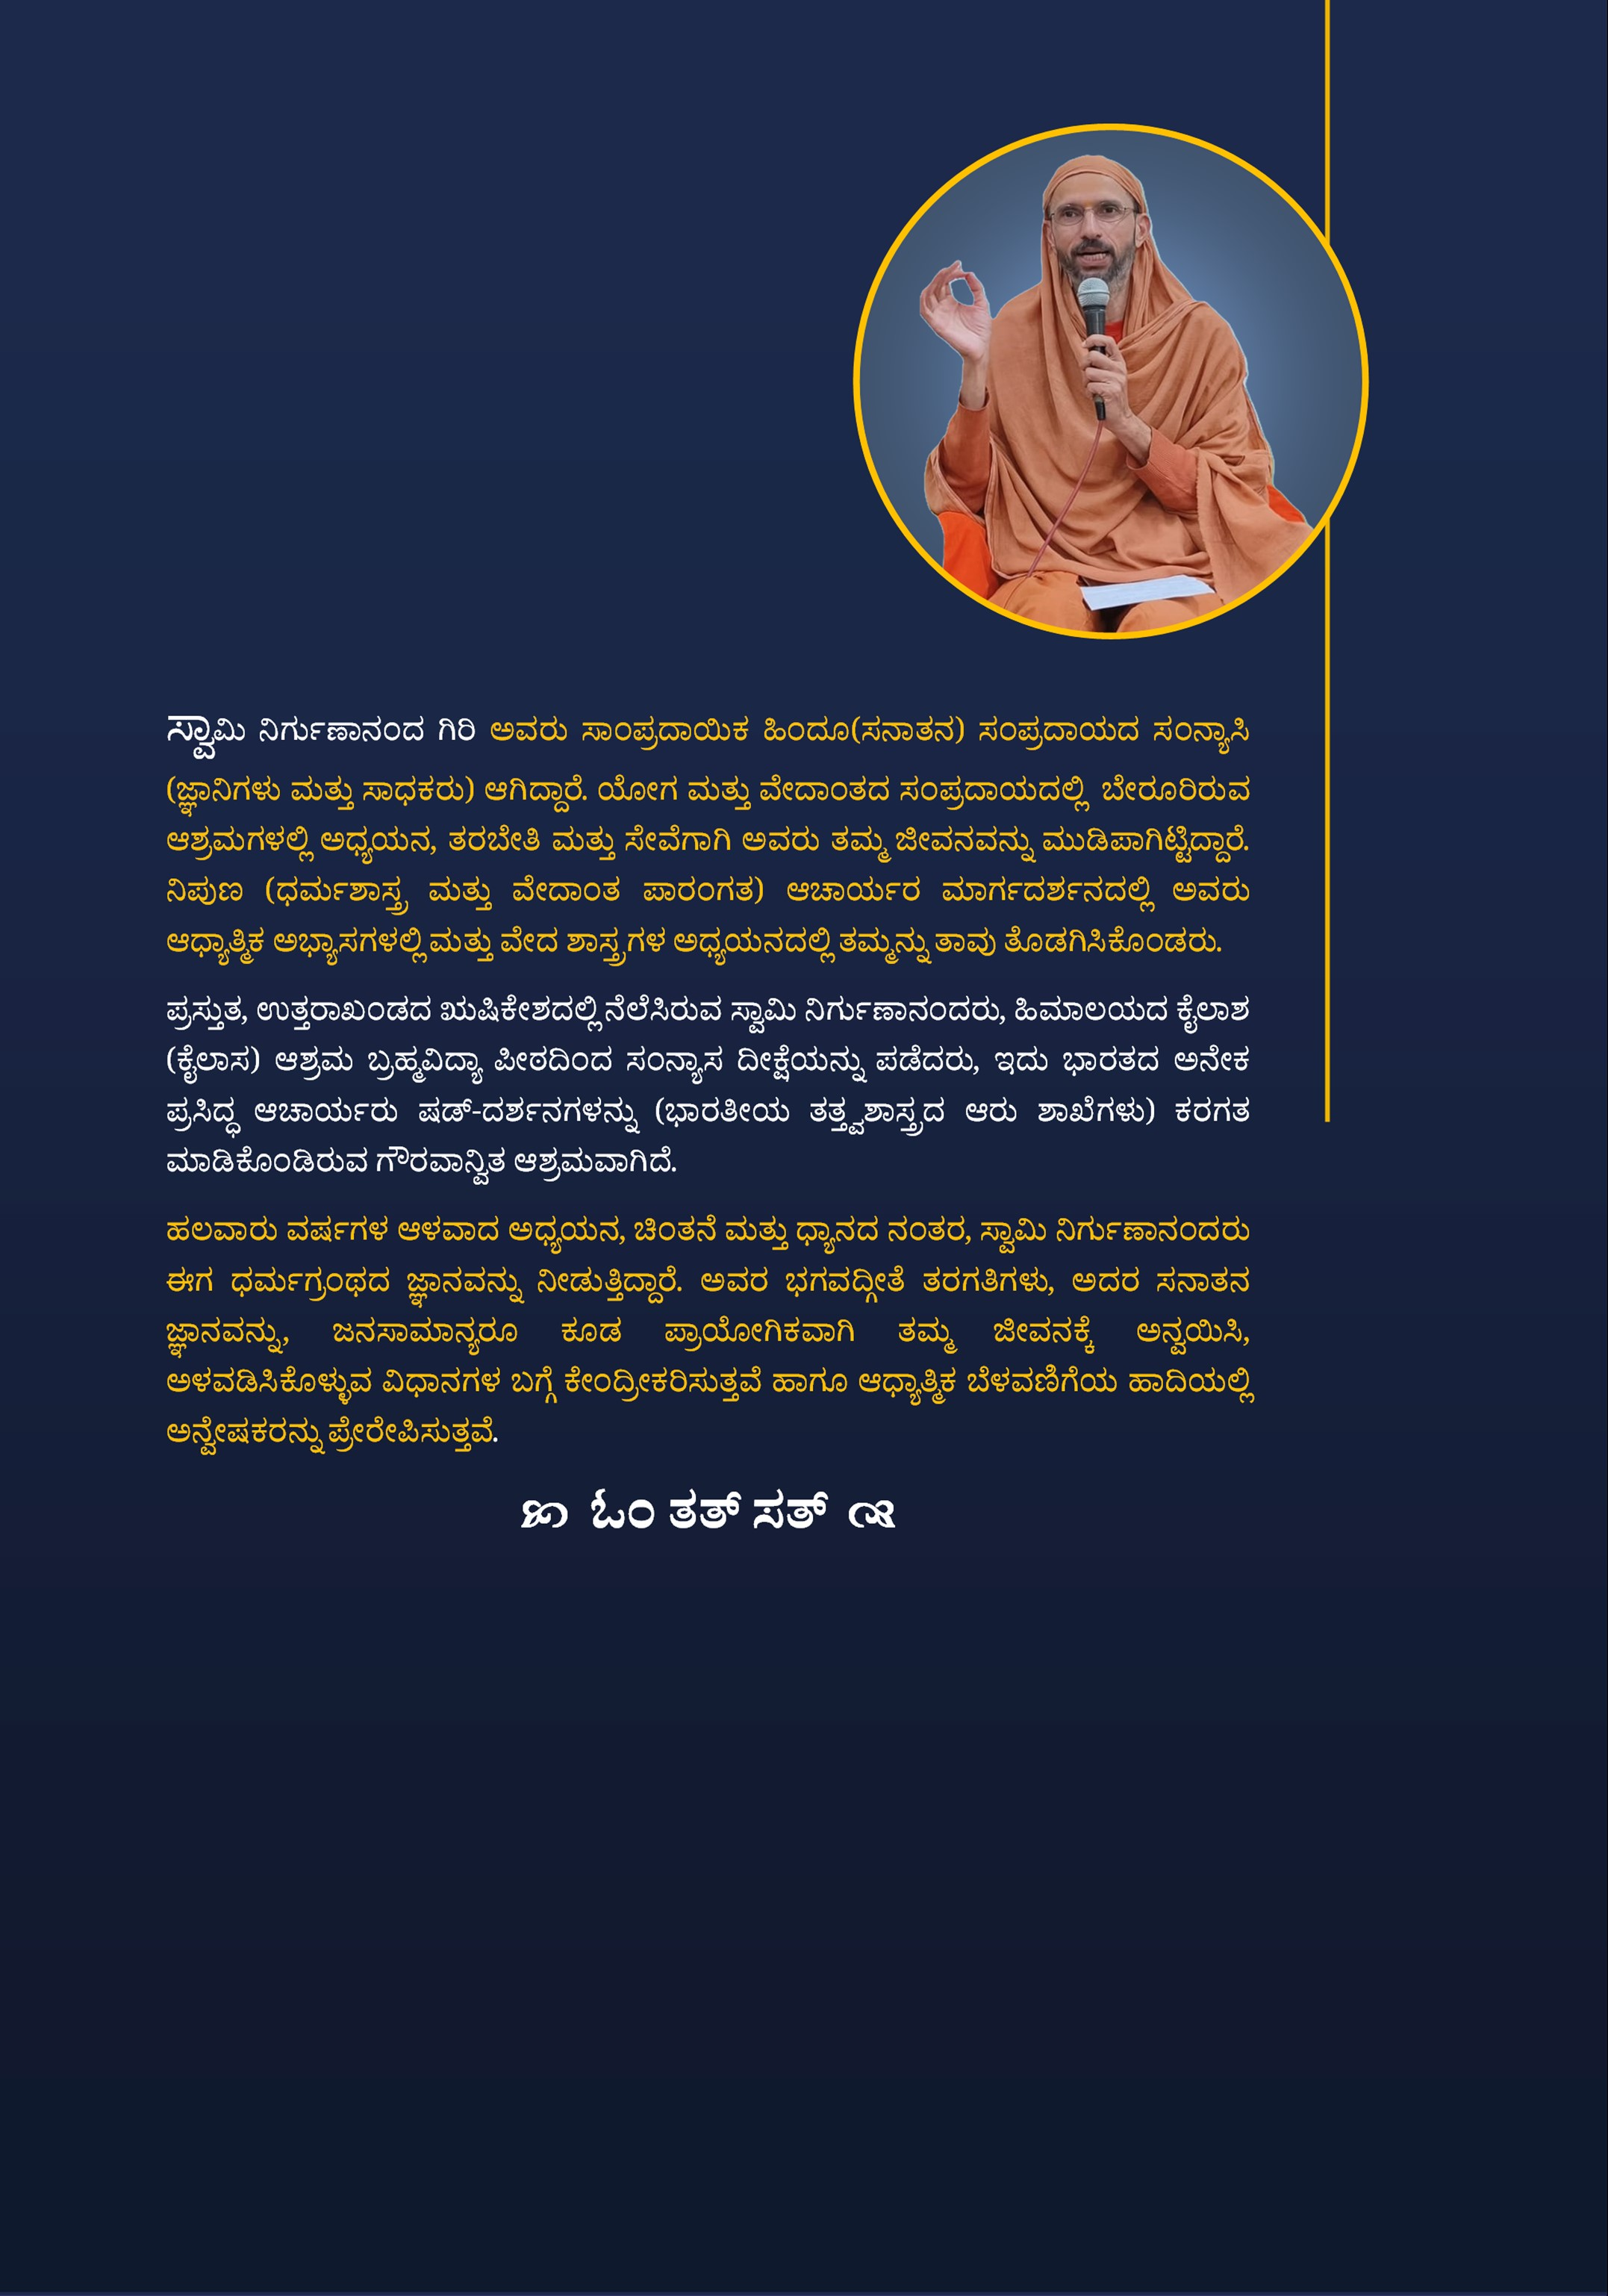
\includegraphics[width=\paperwidth,height=\paperheight]{./images/page02.jpg}%
    }%
	}
   \else% do nothing
   \AddToShipoutPictureBG*{%
    \AtPageLowerLeft{%
        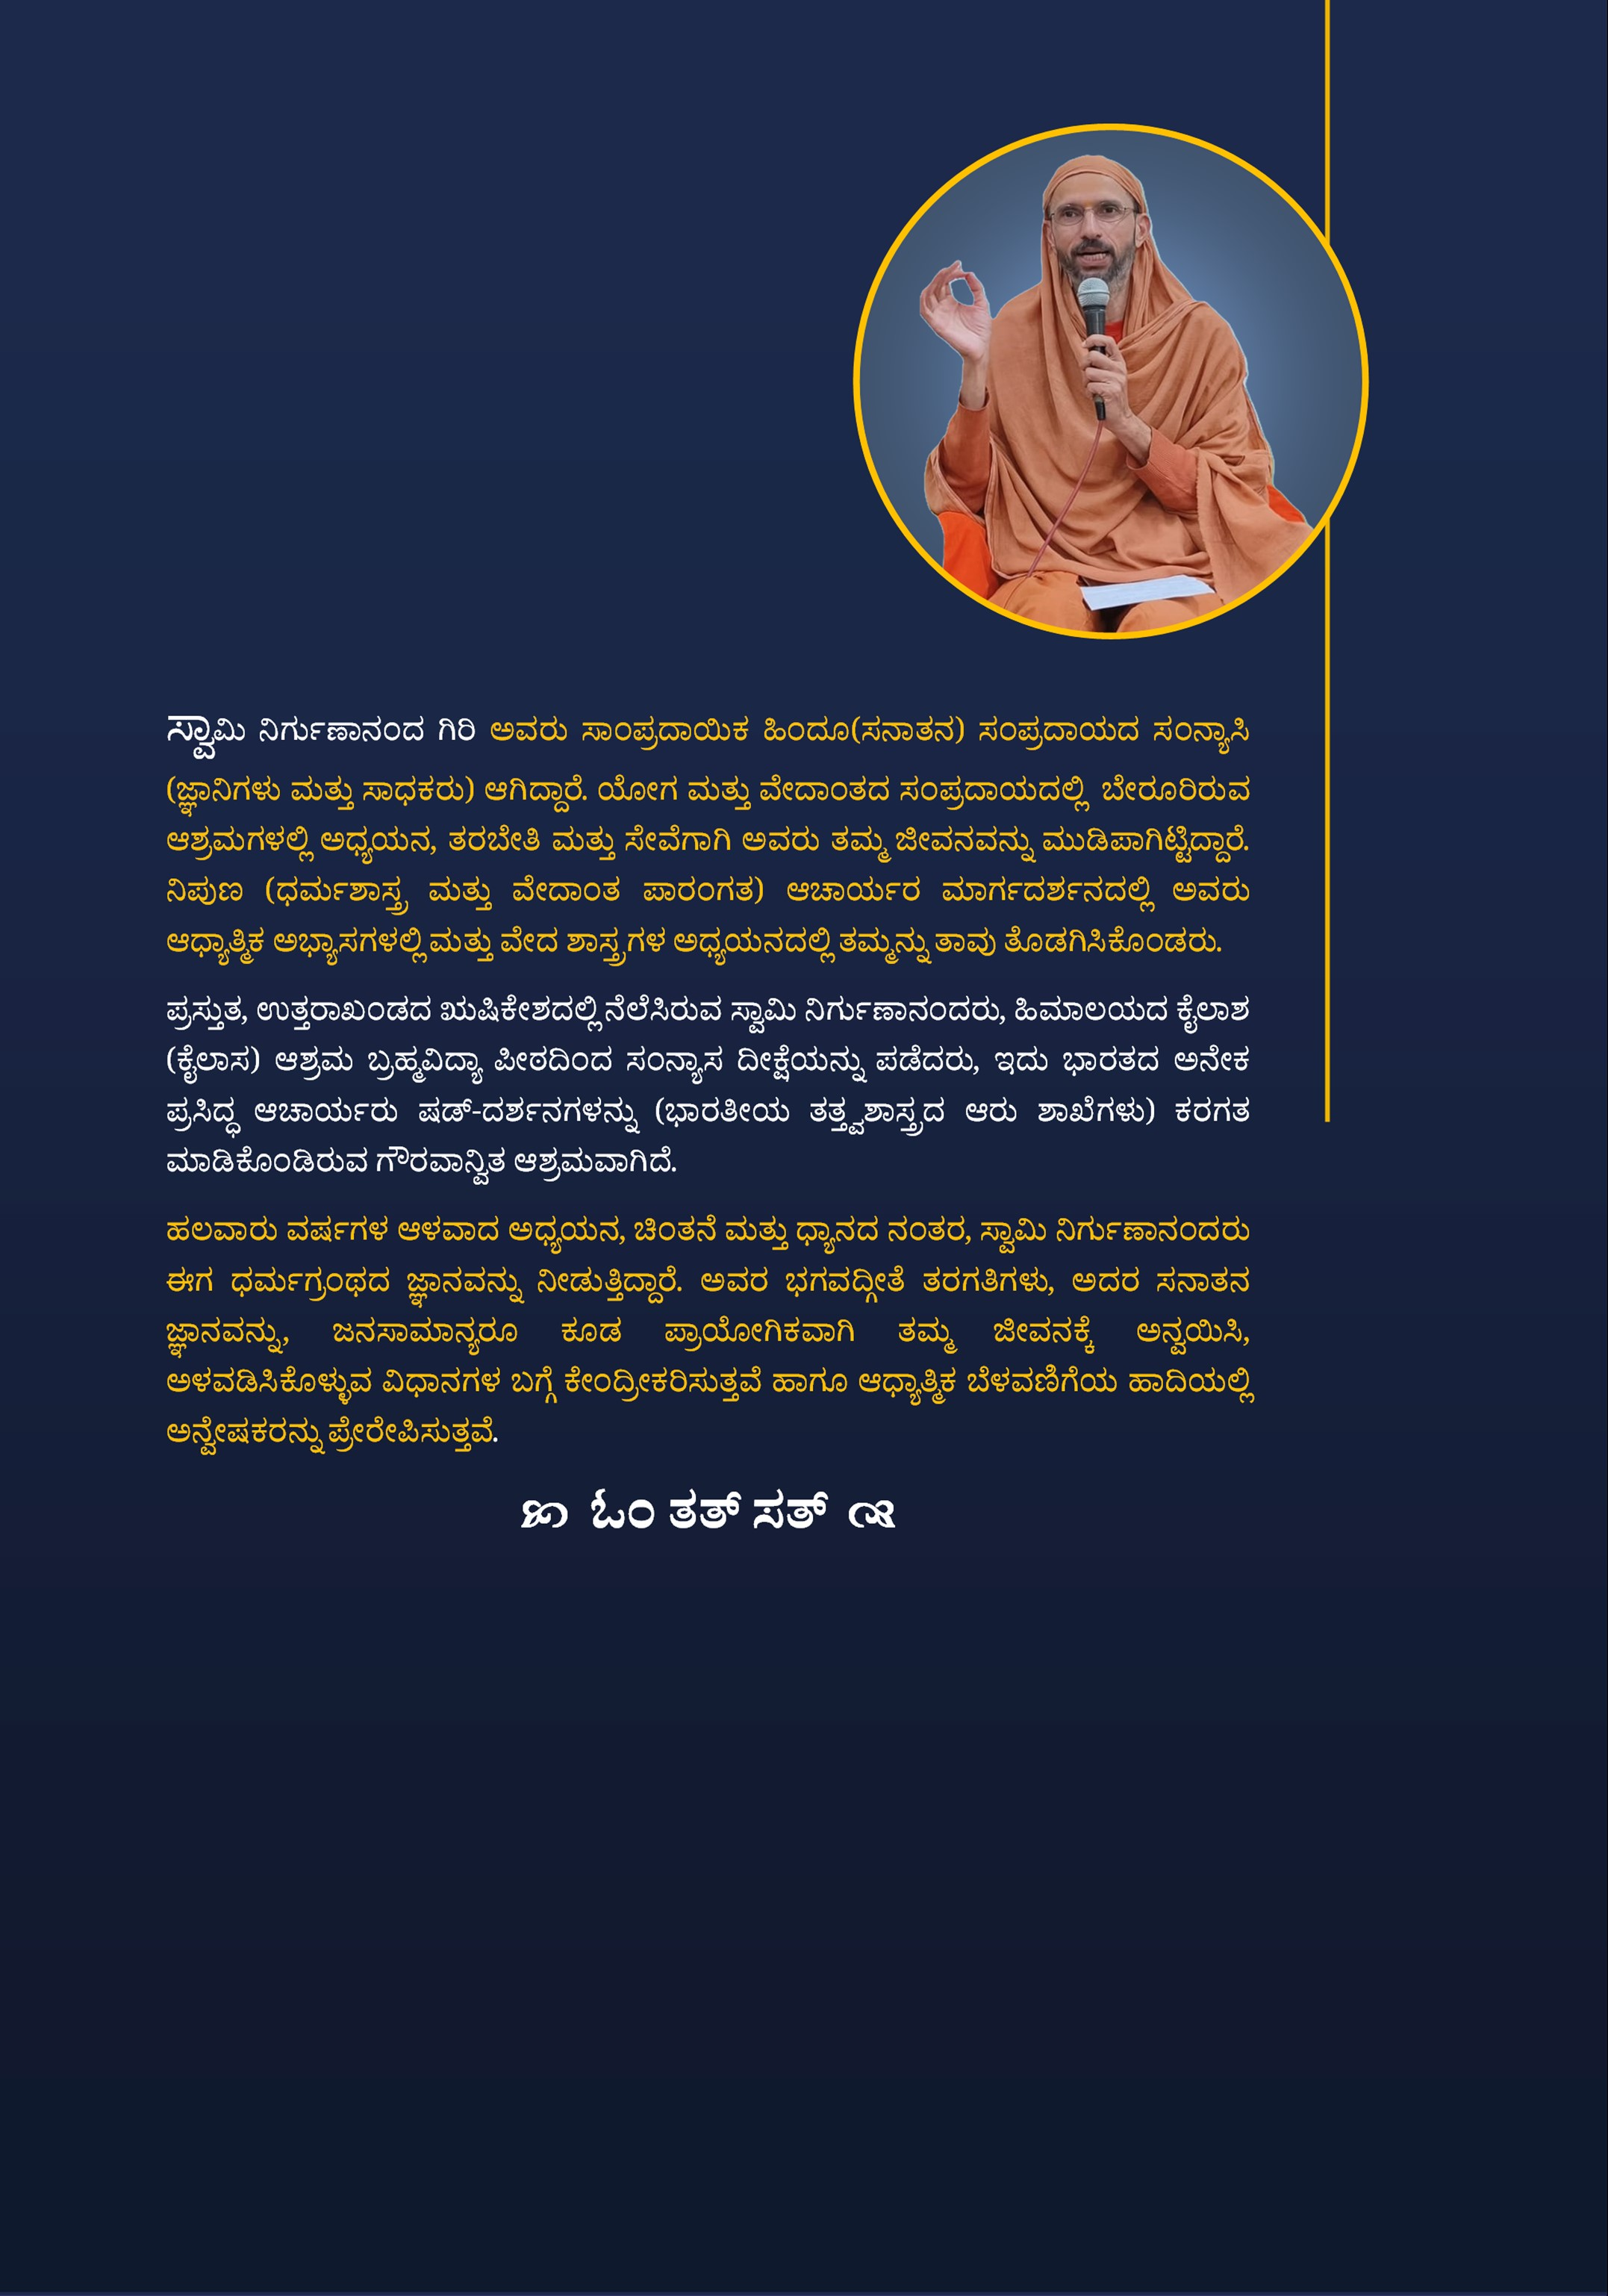
\includegraphics[width=\paperwidth,height=\paperheight]{./images/page02.jpg}%
    }%
	}
\fi
\begin{titlepage}
	%\pagecolor{pastelblue}
	\AddToShipoutPictureBG*{%
    \AtPageLowerLeft{%
        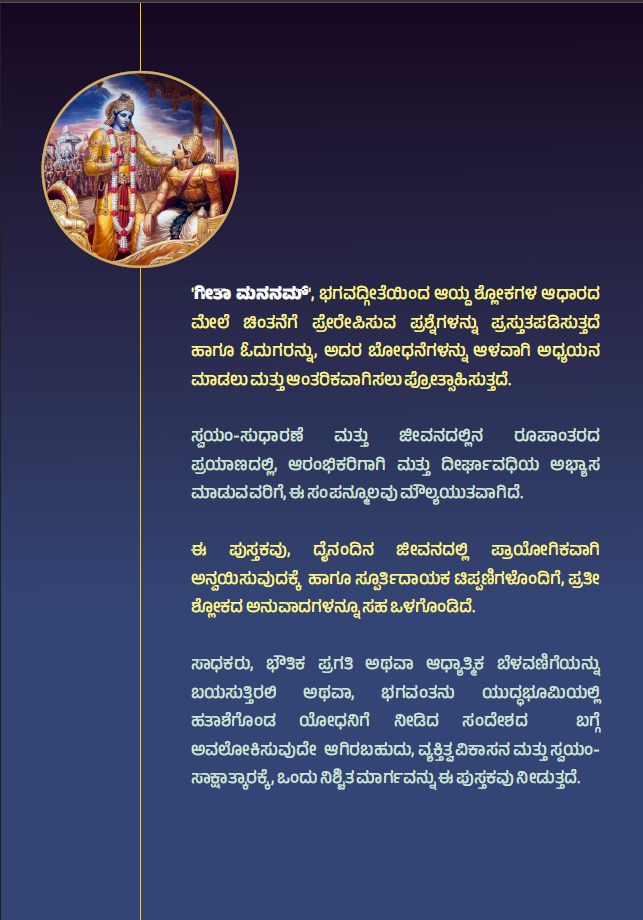
\includegraphics[width=\paperwidth,height=\paperheight]{./images/backcover.png}%
    }%
}
    \begin{center}
        \vspace*{0.5cm}
            
        {\Huge
        %\textbf{\color{white}\fontsize{50}{60}\selectfont ಗೀತಾ ಮನನಂ}
		}
        %\textbf{\\ \small \color{white}ದೈನಂದಿನ ಸ್ಪೂರ್ತಿ ಹಾಗೂ ಆತ್ಮಾವಲೋಕನಕ್ಕಾಗಿ}    
        \vspace{1.0cm}
            
        
		
            
        \vfill
            
        
            
        \vspace{0.1cm}
        {\color{white}    
		%\textbf{{\Large \mananamfont ಸ್ವಾಮಿ ನಿರ್ಗುಣಾನಂದ ಗಿರಿ}}\\
		%{\normalsize Swami Nirgunananda Giri\\Rishikesh, India}
        }
    \end{center}
\end{titlepage}
\nopagecolor% Use this to restore the color pages to white
\end{document}
